\section{Experimental Results}

\subsection{Tables of Most Significant Performance}
Tables \ref{table:first_param_table} through \ref{table:last_param_table} show metrics for the top and bottom 10 performing HOG parameter configurations at both the individual dataset level and across the aggregate test sample. The tables for the performance scores of every parameter configuration are available in appendix \ref{appendix:tables_of_data}.
\subsubsection{Tables of Most Performant Parameters}\label{section:best_tables}

\begin{table}
    \centering
    \includegraphics[width=0.9\linewidth]{../tables/top10/INRIA_best_10.png}
    \caption{Top 10 performing HOG parameter configurations on the INRIA data set, ranked by MCC}
    \label{table:first_param_table}
\end{table}

\begin{table}
    \centering
    \includegraphics[width=0.9\linewidth]{../tables/top10/caltech_30_best_10.png}
    \caption{Top 10 performing HOG parameter configurations on the Caltech data set, ranked by MCC}
\end{table}

\begin{table}
    \centering
    \includegraphics[width=0.9\linewidth]{../tables/top10/PnPLO_best_10.png}
    \caption{Top 10 performing HOG parameter configurations on the PnPLO data set, ranked by MCC}
\end{table}

\begin{table}
    \centering
    \includegraphics[width=0.9\linewidth]{../tables/top10/total_best_10.png}
    \caption{Top 10 performing HOG parameter configurations on the aggregate test data set, ranked by MCC}
\end{table}

\subsubsection{Tables of Least Performant Parameters}\label{section:worst_tables}

\begin{table}
    \centering
    \includegraphics[width=0.9\linewidth]{../tables/top10/INRIA_worst_10.png}
    \caption{Bottom 10 performing HOG parameter configurations on the INRIA data set, ranked by MCC}
\end{table}

\begin{table}
    \centering
    \includegraphics[width=0.9\linewidth]{../tables/top10/caltech_30_worst_10.png}
    \caption{Bottom 10 performing HOG parameter configurations on the Caltech data set, ranked by MCC}
\end{table}

\begin{table}
    \centering
    \includegraphics[width=0.9\linewidth]{../tables/top10/PnPLO_worst_10.png}
    \caption{Bottom 10 performing HOG parameter configurations on the PnPLO data set, ranked by MCC}
\end{table}

\begin{table}
    \centering
    \includegraphics[width=0.9\linewidth]{../tables/top10/total_worst_10.png}
    \caption{Bottom 10 performing HOG parameter configurations on the aggregate test data set, ranked by MCC}
    \label{table:last_param_table}
\end{table}

\subsection{Graphical Presentation of Individual Parameter Influence}

While tables in \ref{section:best_tables} and \ref{section:worst_tables} show the best and worst parameter combinations, they don't reveal how individual parameters affect performance. To analyze this, models are grouped into sets based on shared parameter values and compared with models that differ by only one parameter (models that deviate by the single parameter share a "set index") . To better discern the trend of each individual graph, the MCC score values are uniformly filtered by taking the arithmetic average of each pixel with its neighbor (as implemented in scipy's \href{https://docs.scipy.org/doc/scipy/reference/generated/scipy.ndimage.uniform_filter1d.html}{uniform\_filter1d}). The highest MCC score for each set is highlighted with a marker.

\subsubsection{Graphs for Different Window Sizes}

\begin{figure}\
    \centering
    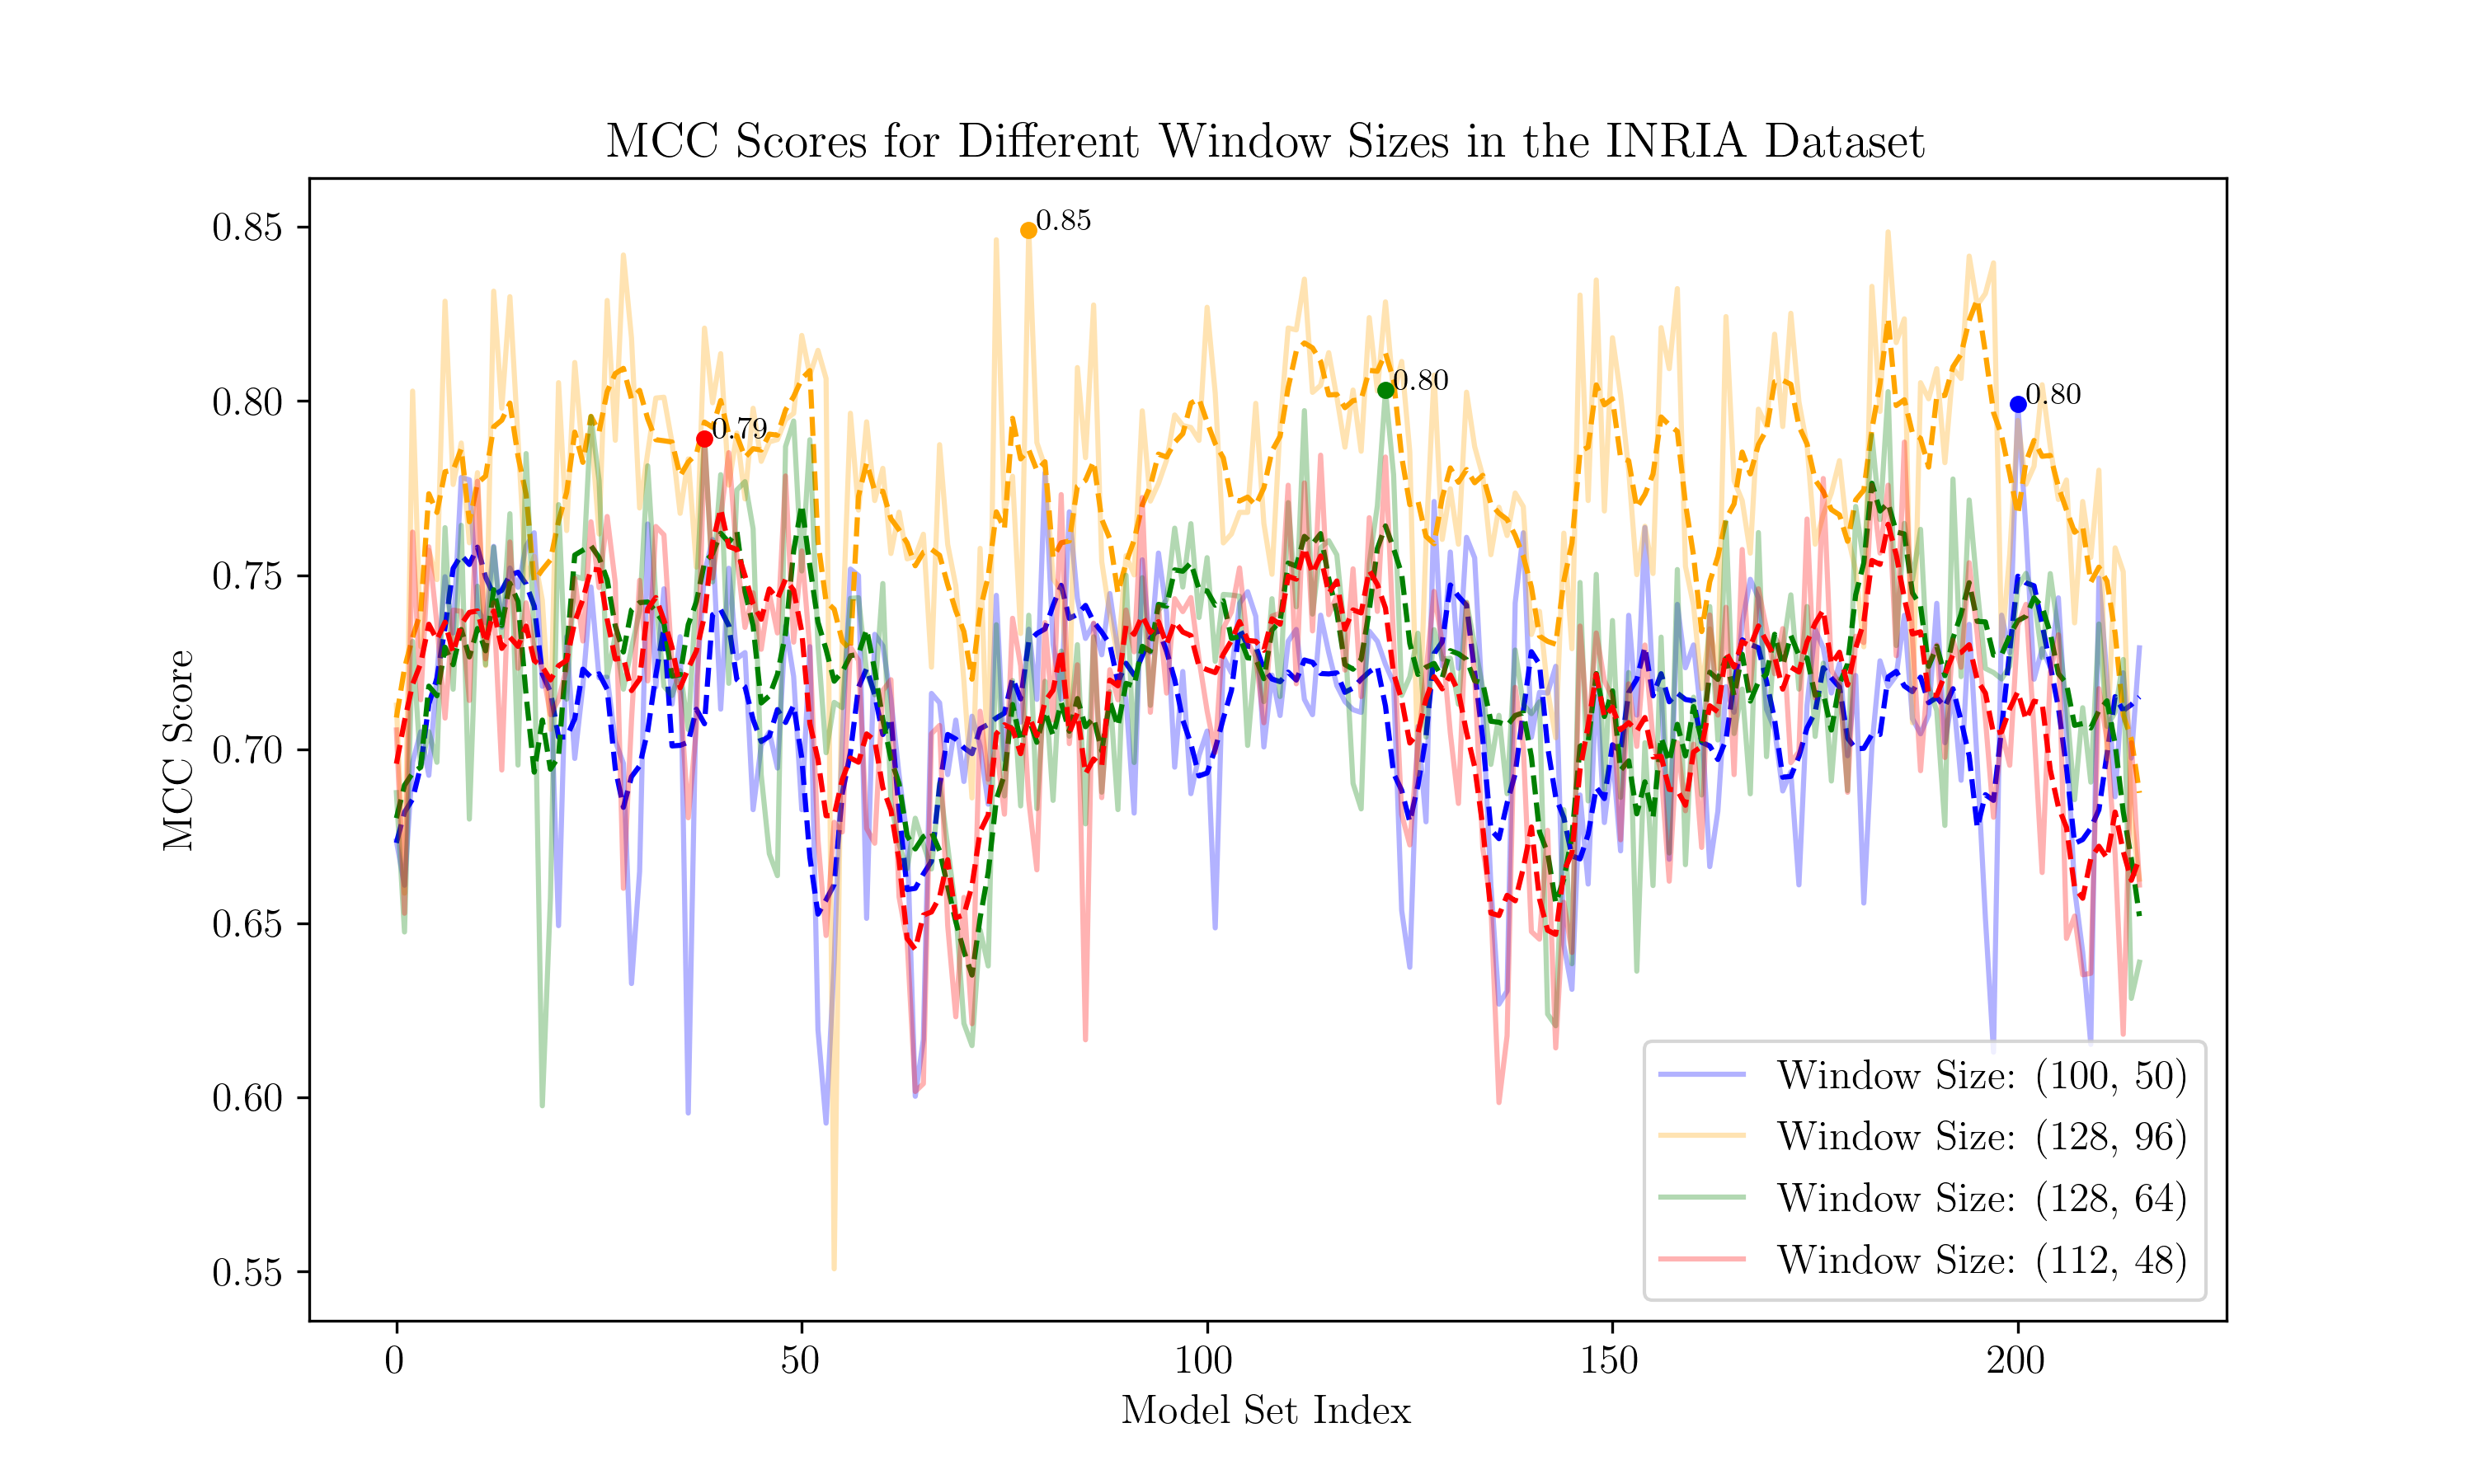
\includegraphics[width=0.9\linewidth]{../images/mcc_windows_INRIA.png}
    \caption{
        MCC scores for INRIA dataset, grouped by window size.
    }
    \label{fig:window_size_inria}
\end{figure}
\begin{figure}
    \centering
    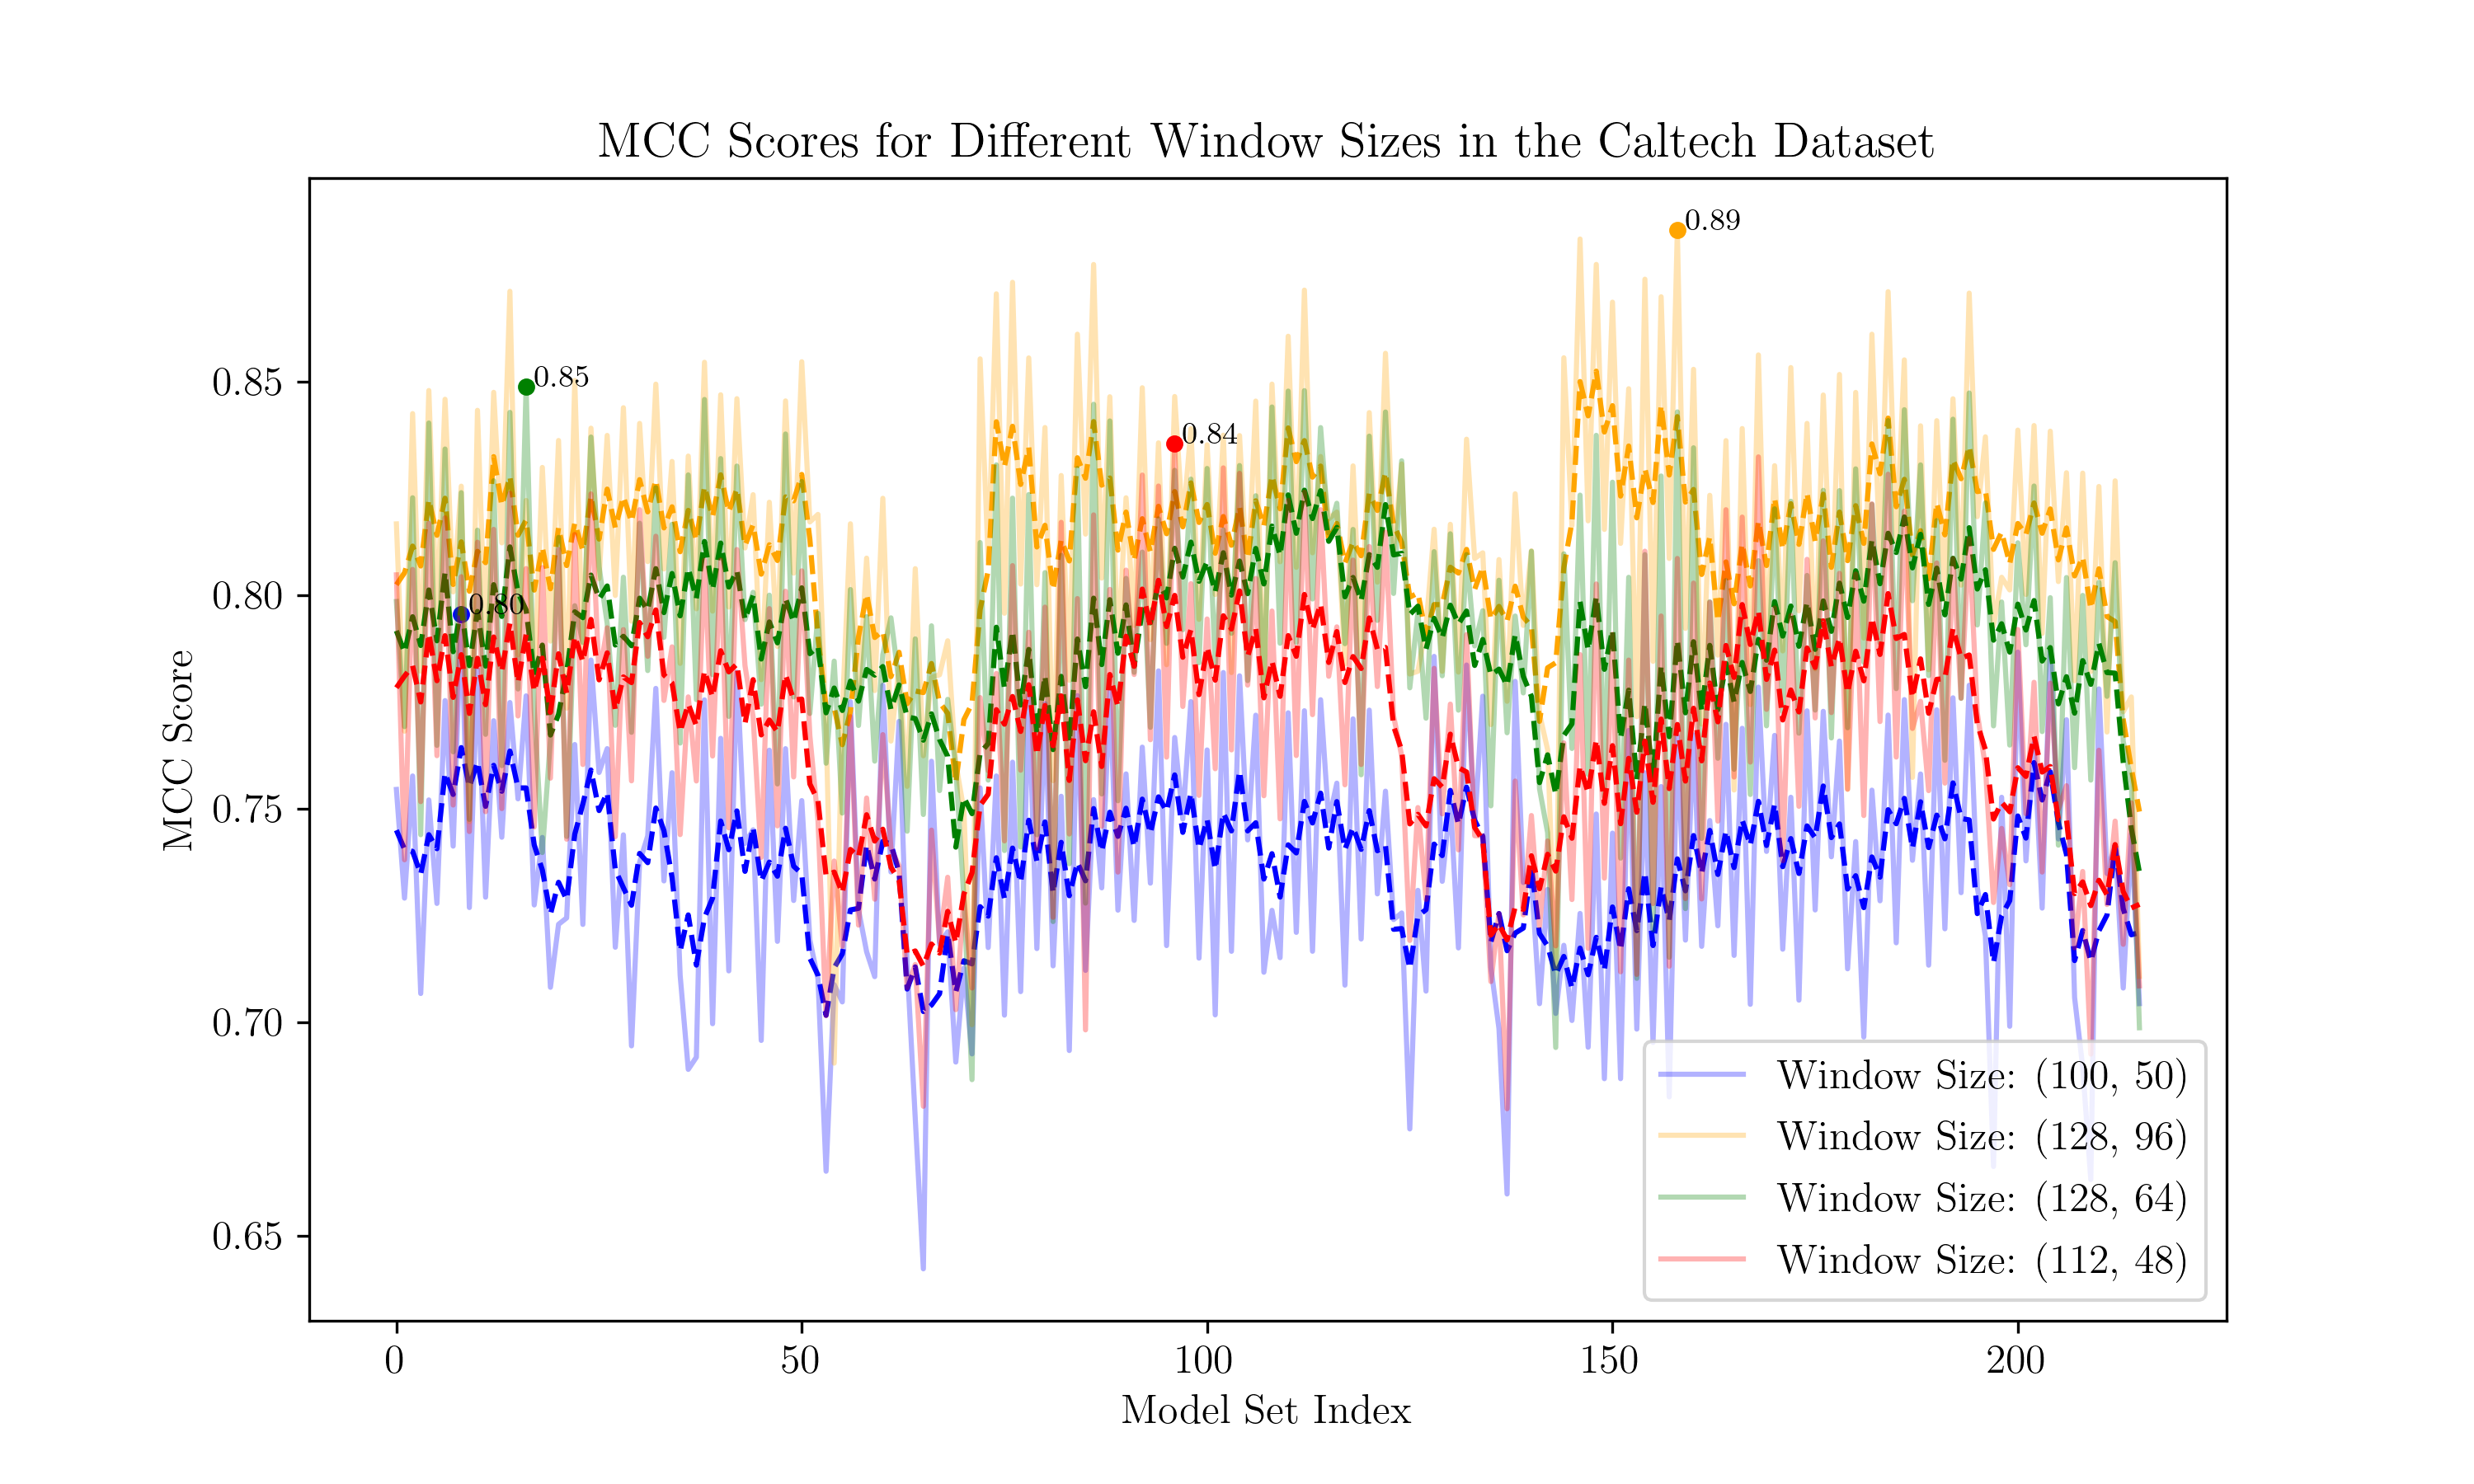
\includegraphics[width=0.9\linewidth]{../images/mcc_windows_caltech_30.png}
    \caption{
        MCC scores for Caltech dataset, grouped by window size.
    }
    \label{fig:window_size_caltech}

\end{figure}
\begin{figure}
    \centering
    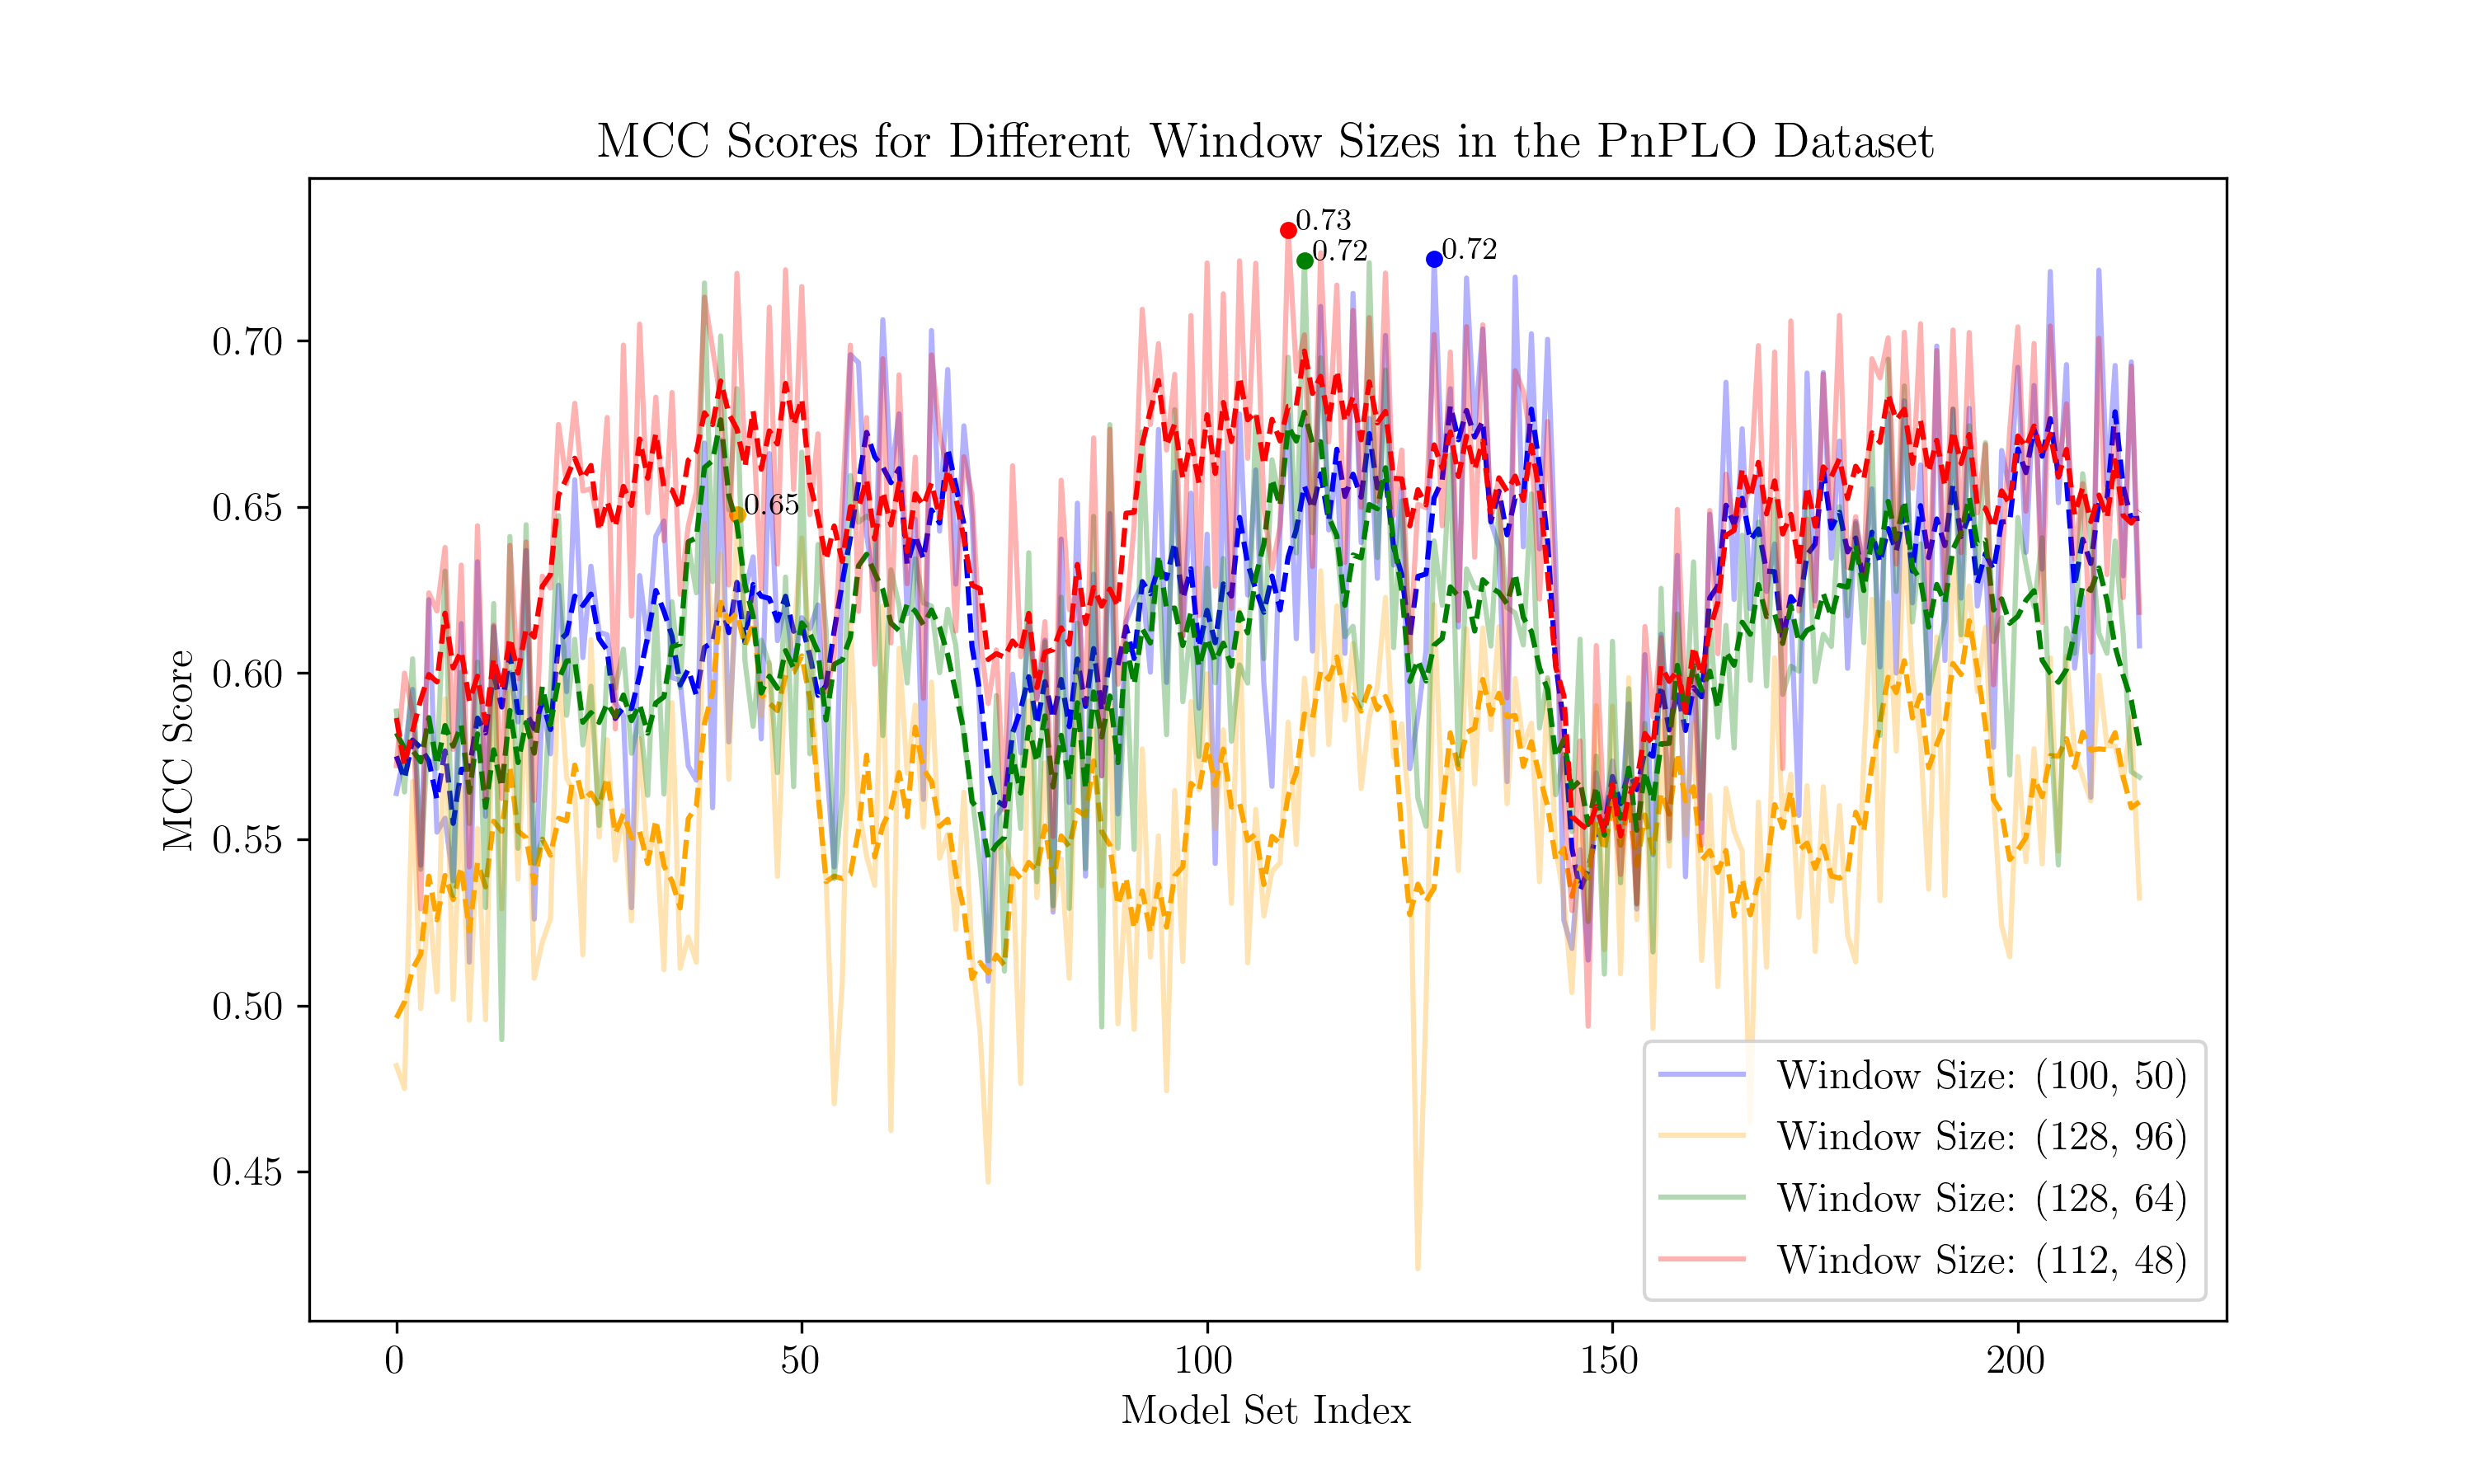
\includegraphics[width=0.9\linewidth]{../images/mcc_windows_PnPLO.png}
    \caption{
        MCC scores for PnPLO dataset, grouped by window size.
    }
    \label{fig:window_size_pnplo}
\end{figure}

\begin{figure}
    \centering
    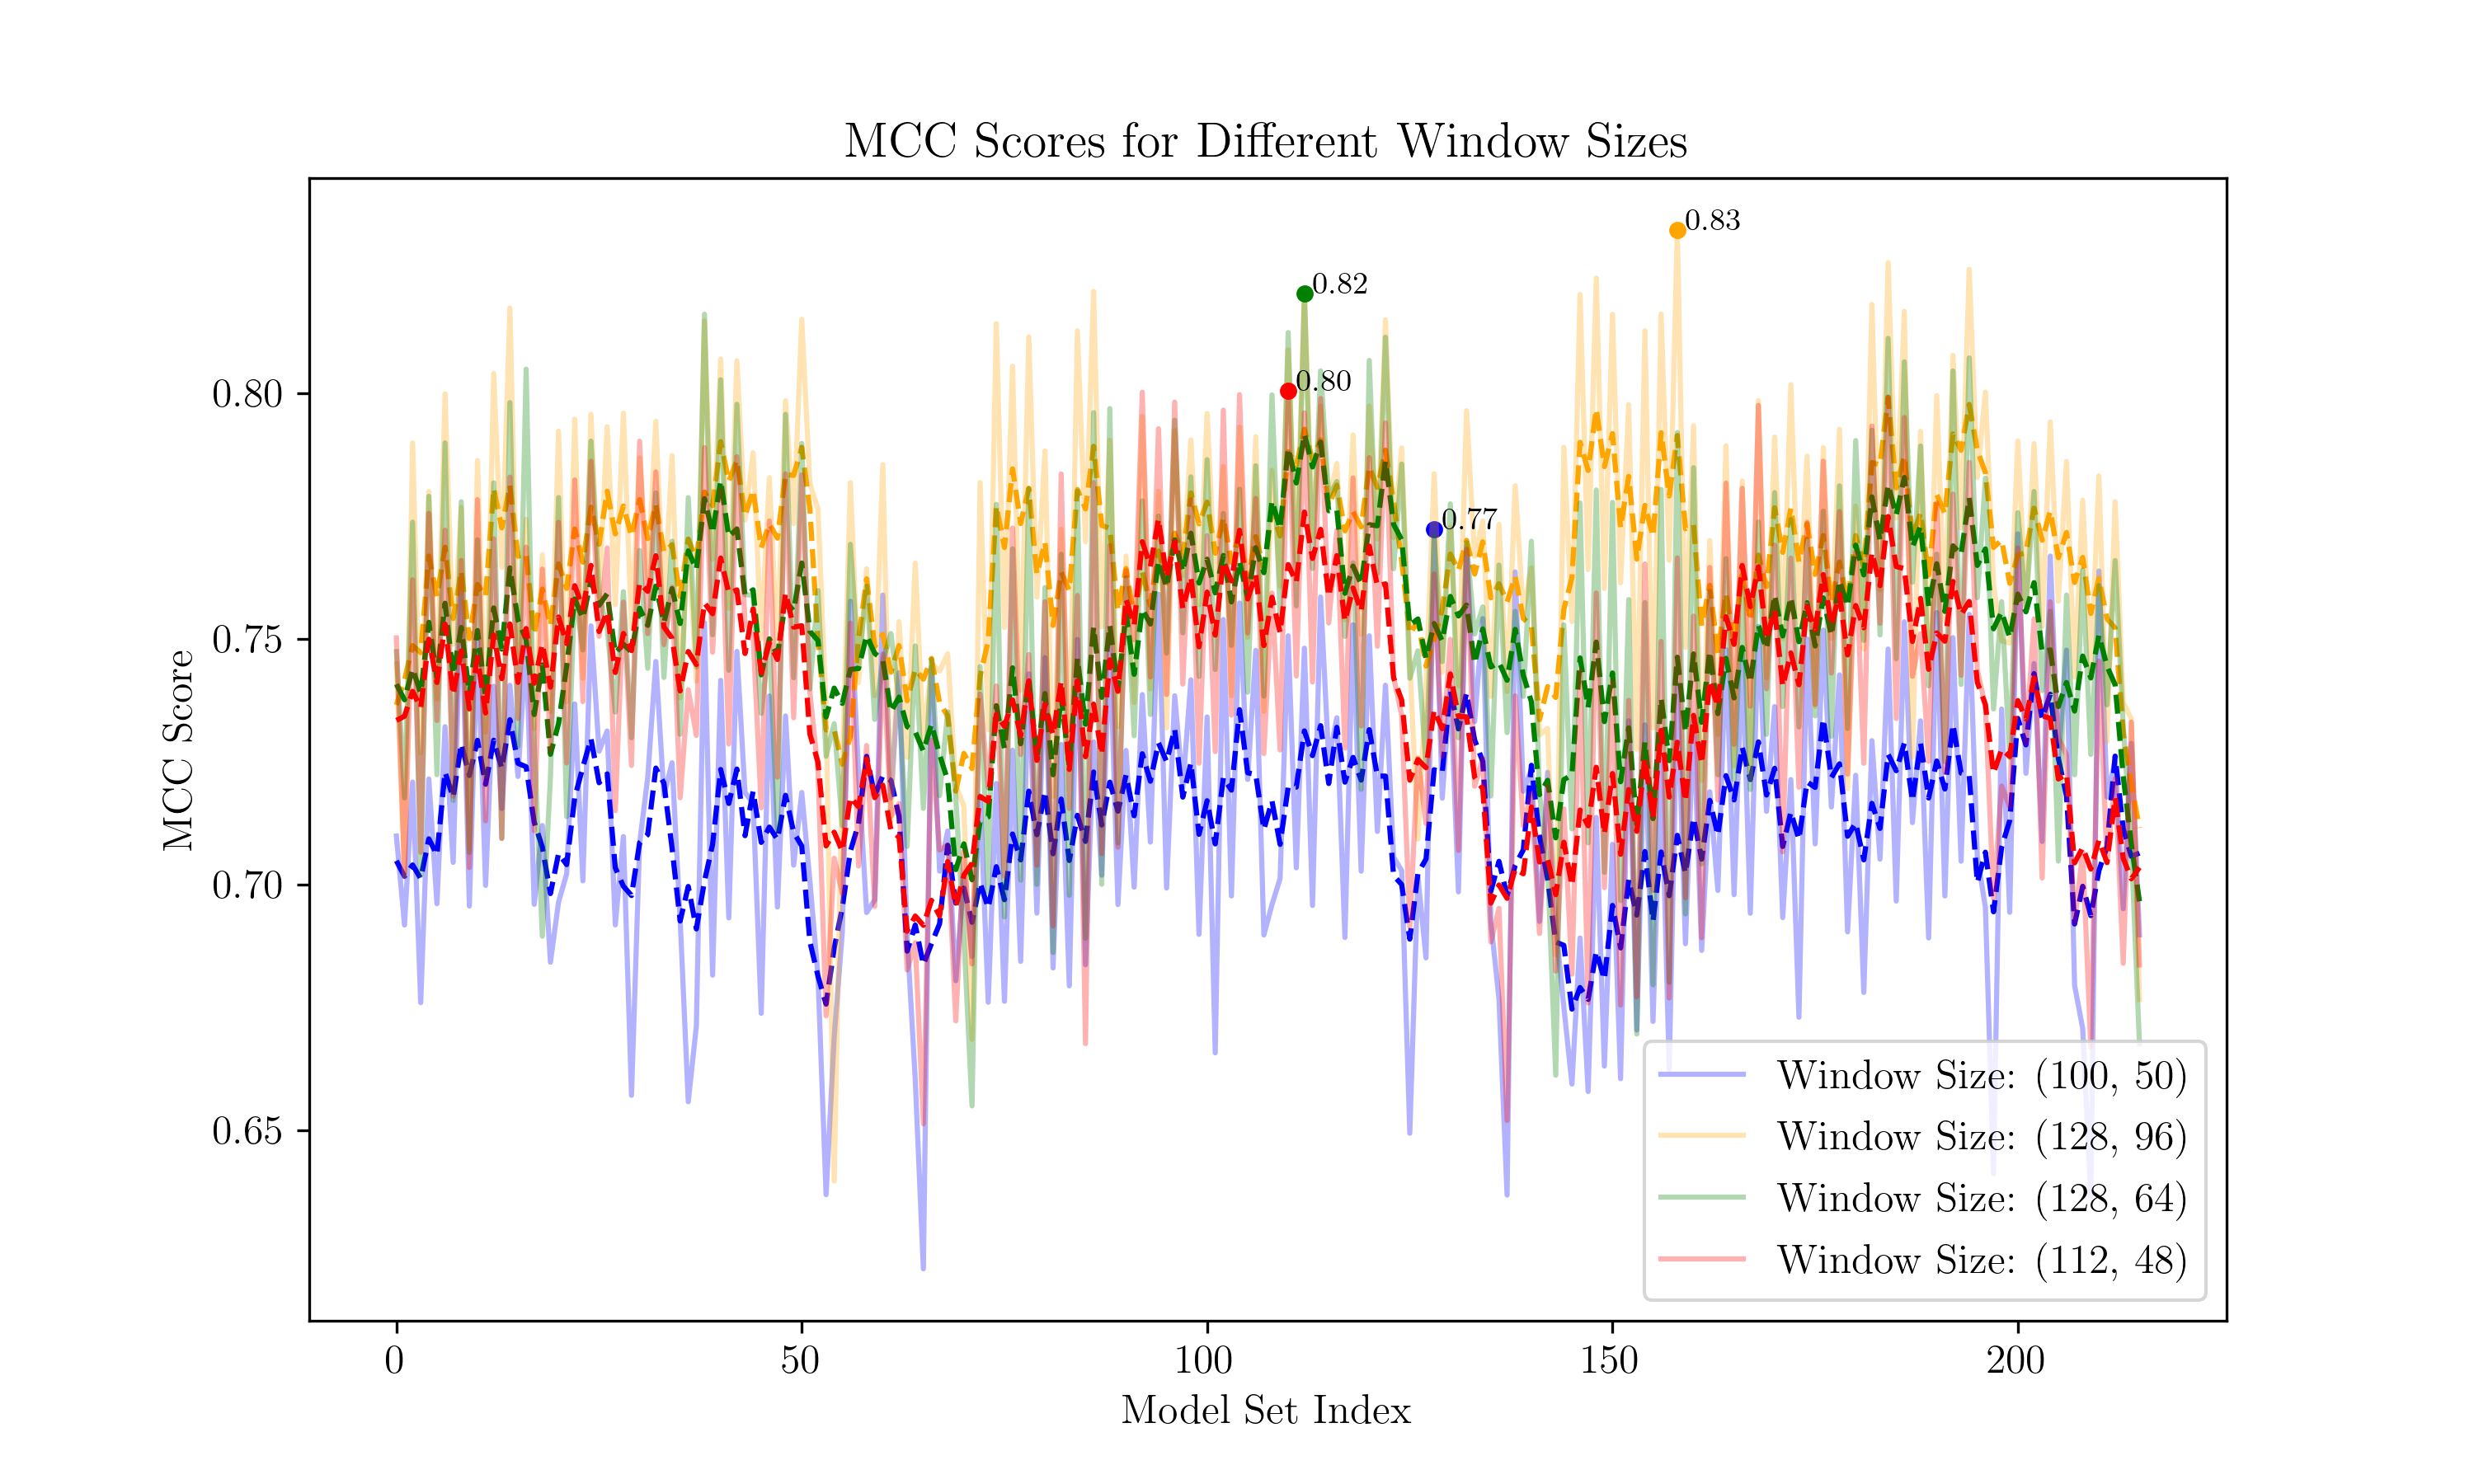
\includegraphics[width=0.9\linewidth]{../images/mcc_windows_total.png}
    \caption{
        MCC scores for the aggregate test dataset, grouped by window size.
    }
\end{figure}

\subsubsection{Graphs for Different Derivative Masks}


\begin{figure}
    \centering
    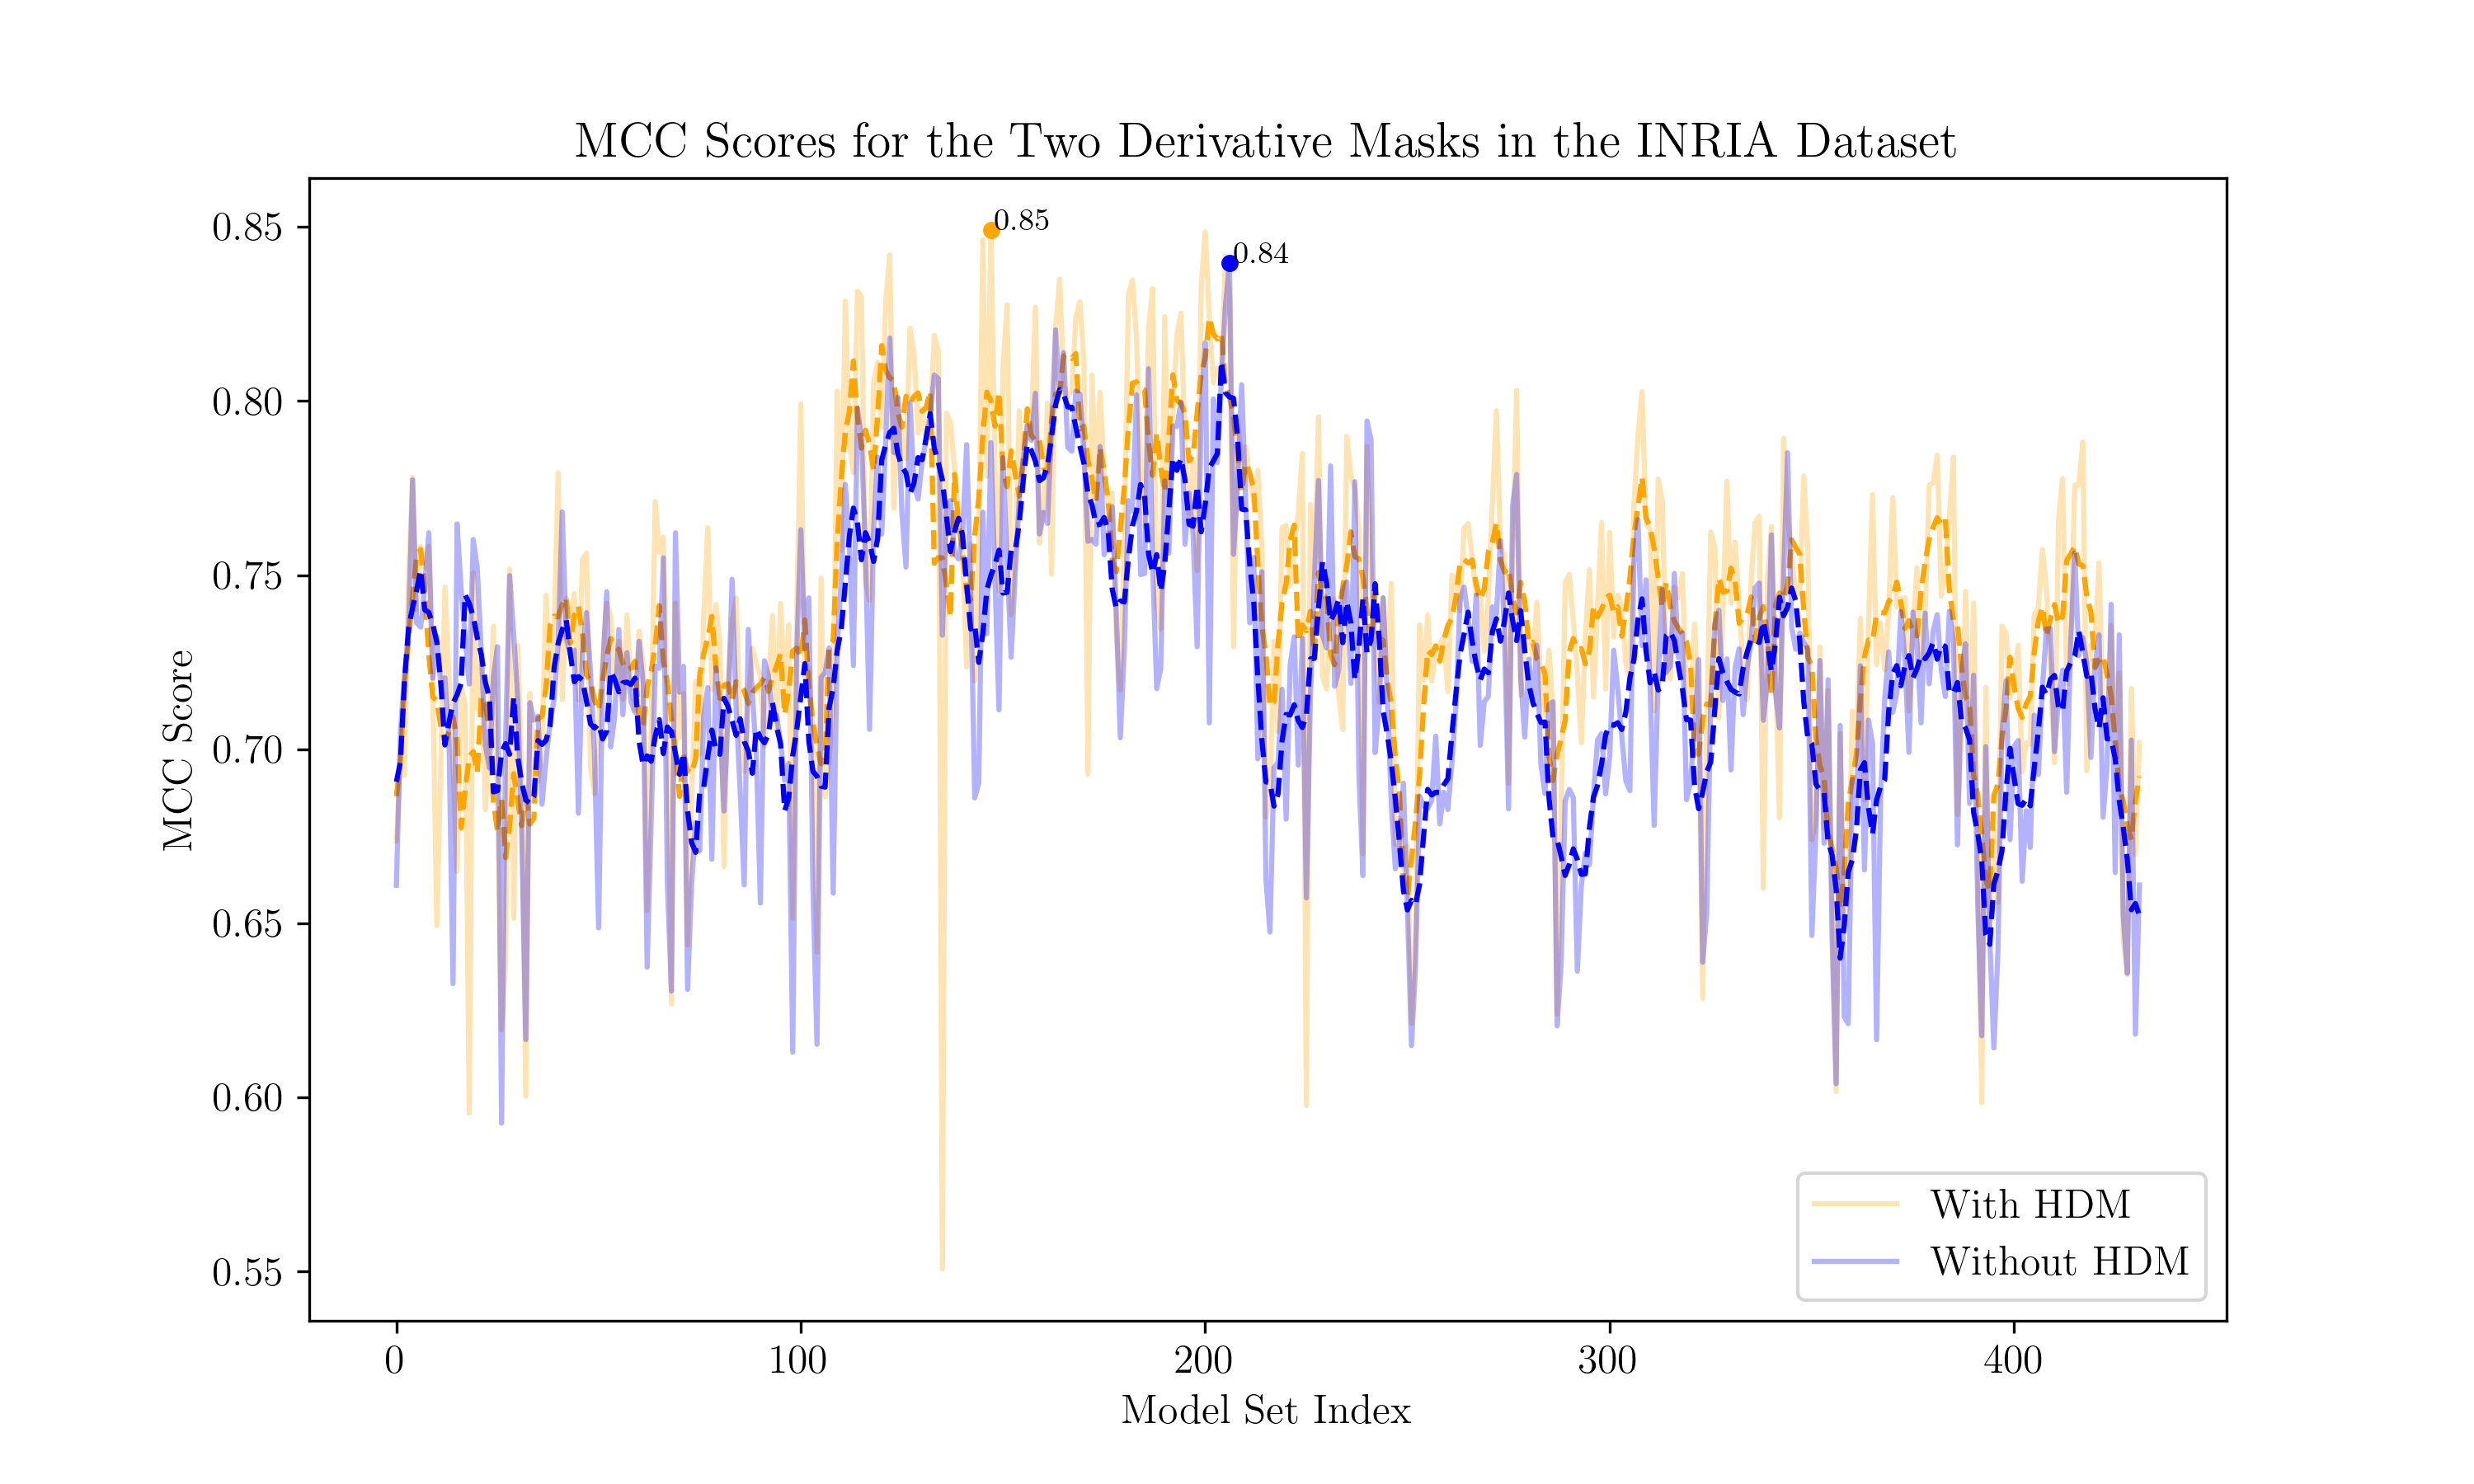
\includegraphics[width=0.9\linewidth]{mcc_hdm_INRIA.png}
    \caption{
        MCC scores for the INRIA dataset, grouped by derivative mask. HDM stands for holistic derivative mask, as introduced in section \ref{sec:deriv_mask}.
    }
    \label{fig:hdm_inria}
\end{figure}
\begin{figure}
    \centering
    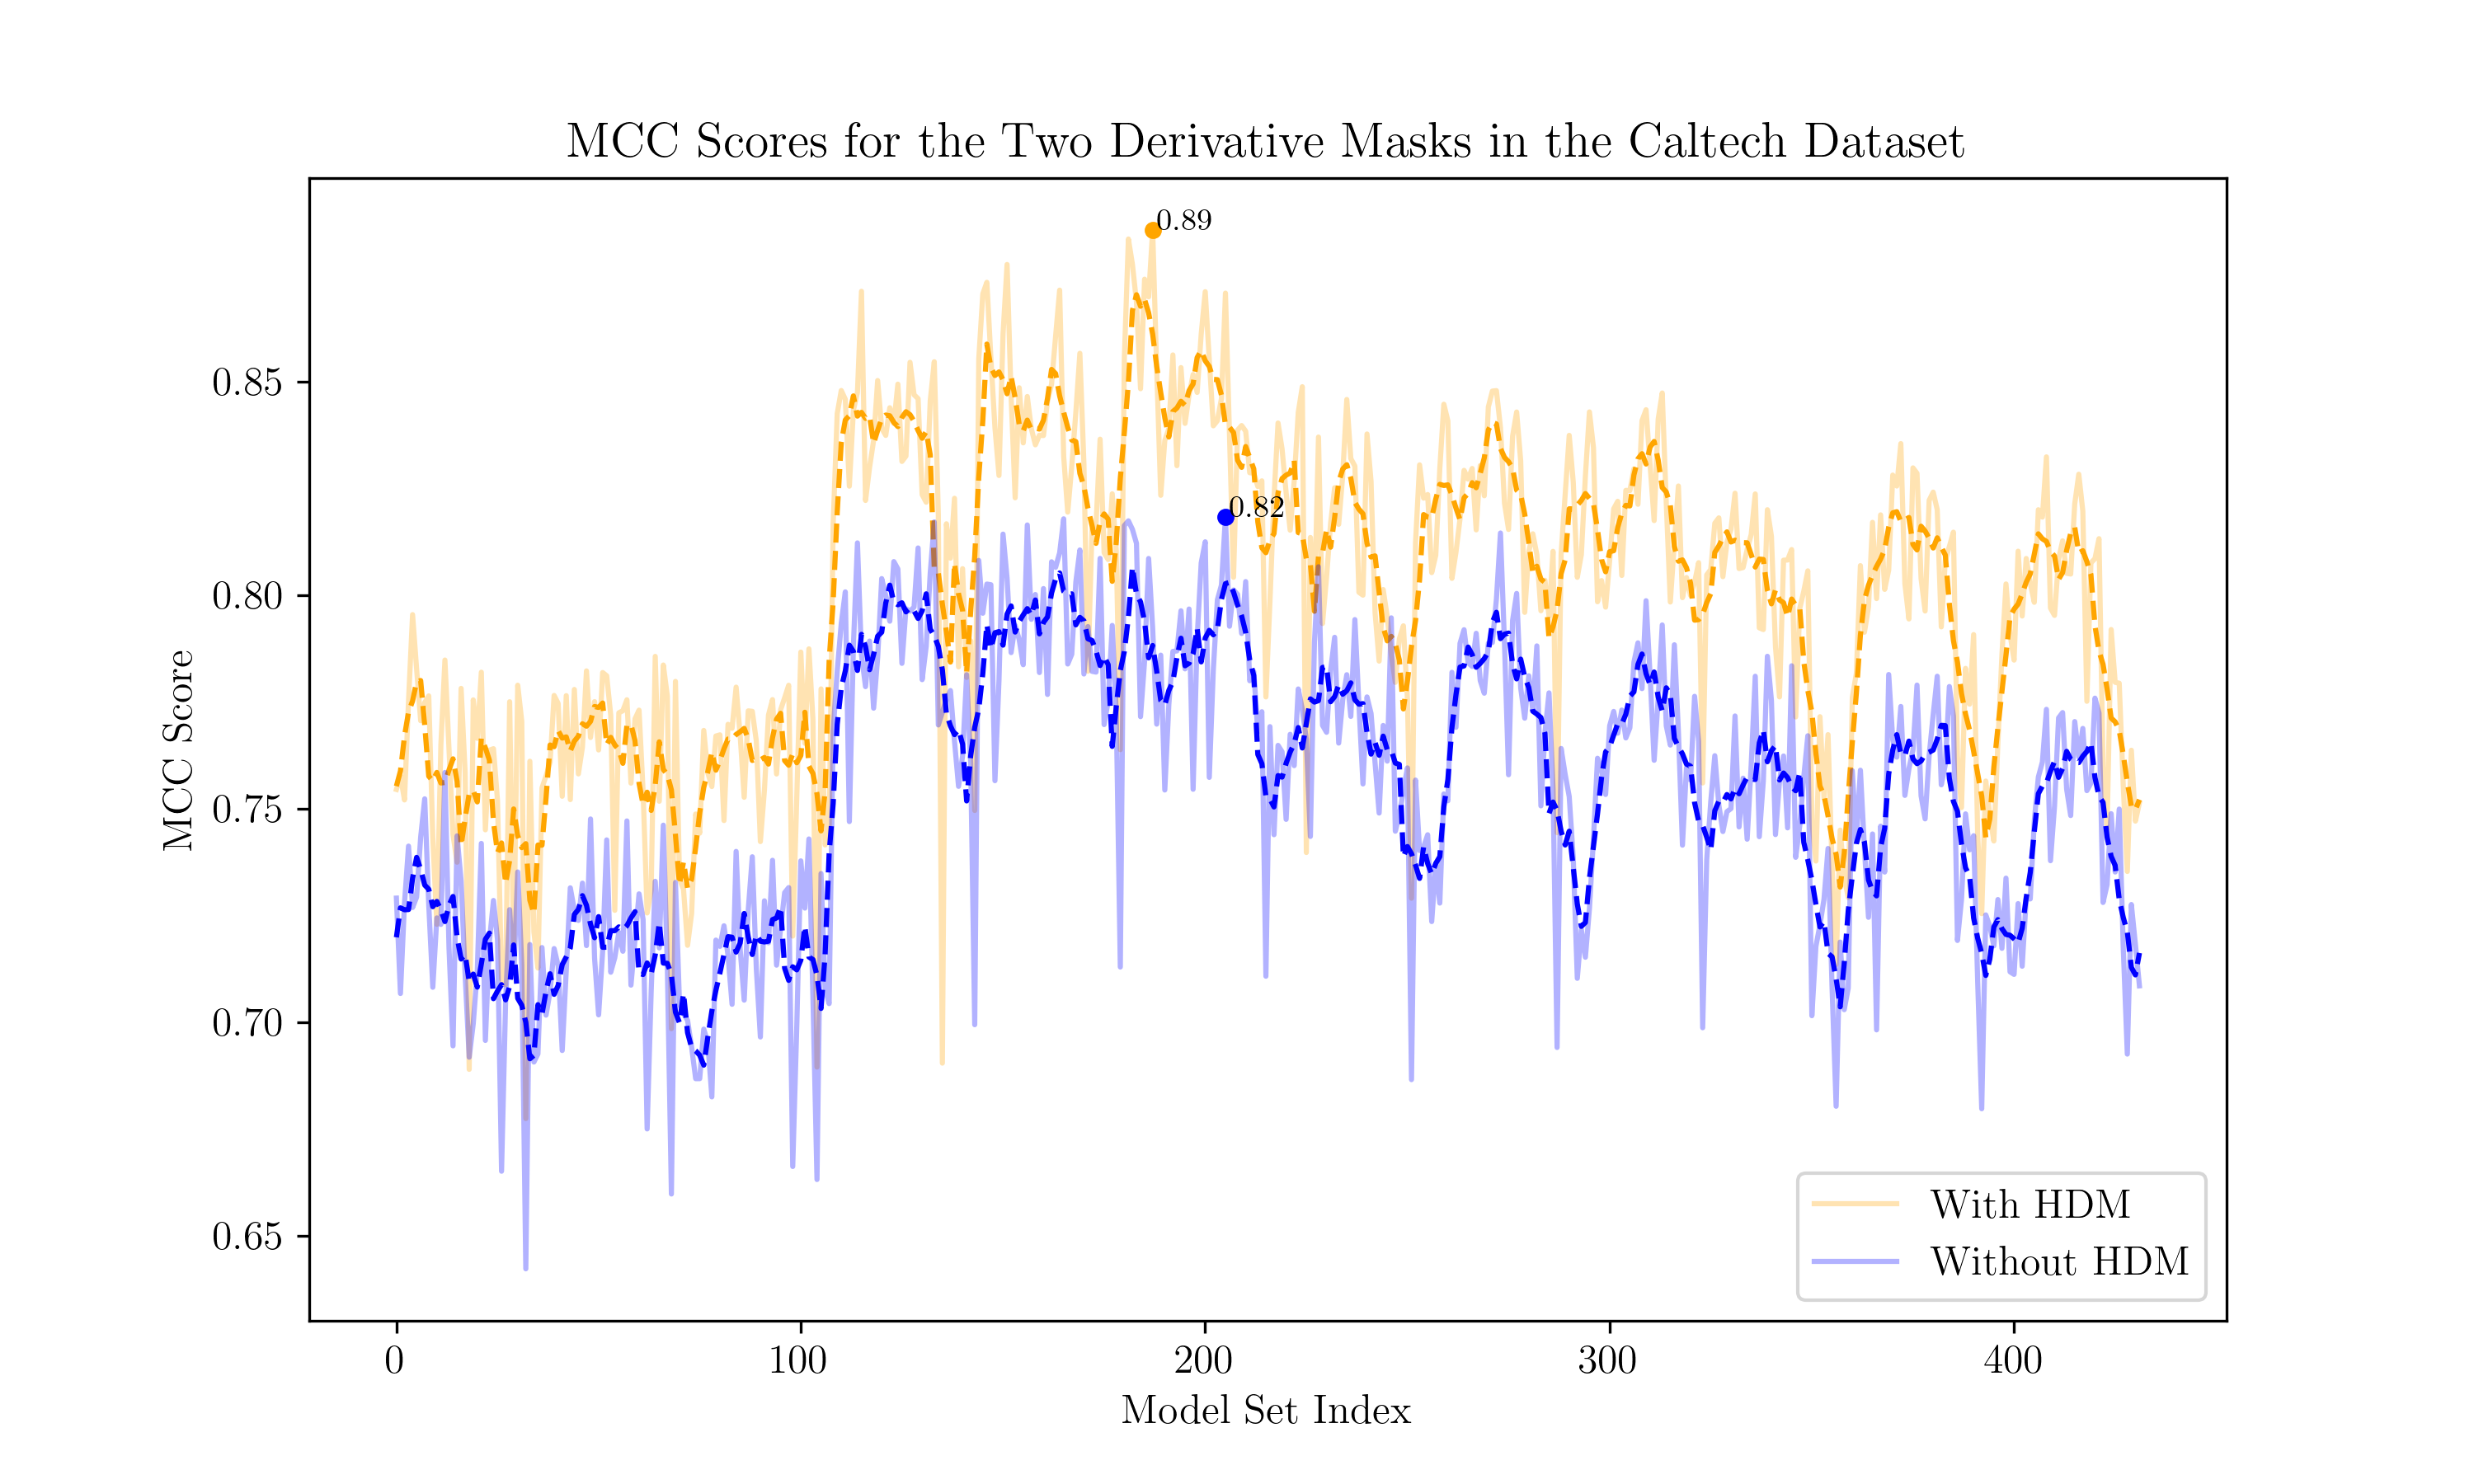
\includegraphics[width=0.9\linewidth]{mcc_hdm_caltech_30.png}
    \caption{
        MCC scores for Caltech dataset, grouped by derivative mask. HDM stands for holistic derivative mask, as introduced in section \ref{sec:deriv_mask}.
    }
    \label{fig:hdm_caltech}
\end{figure}
\begin{figure}
    \centering
    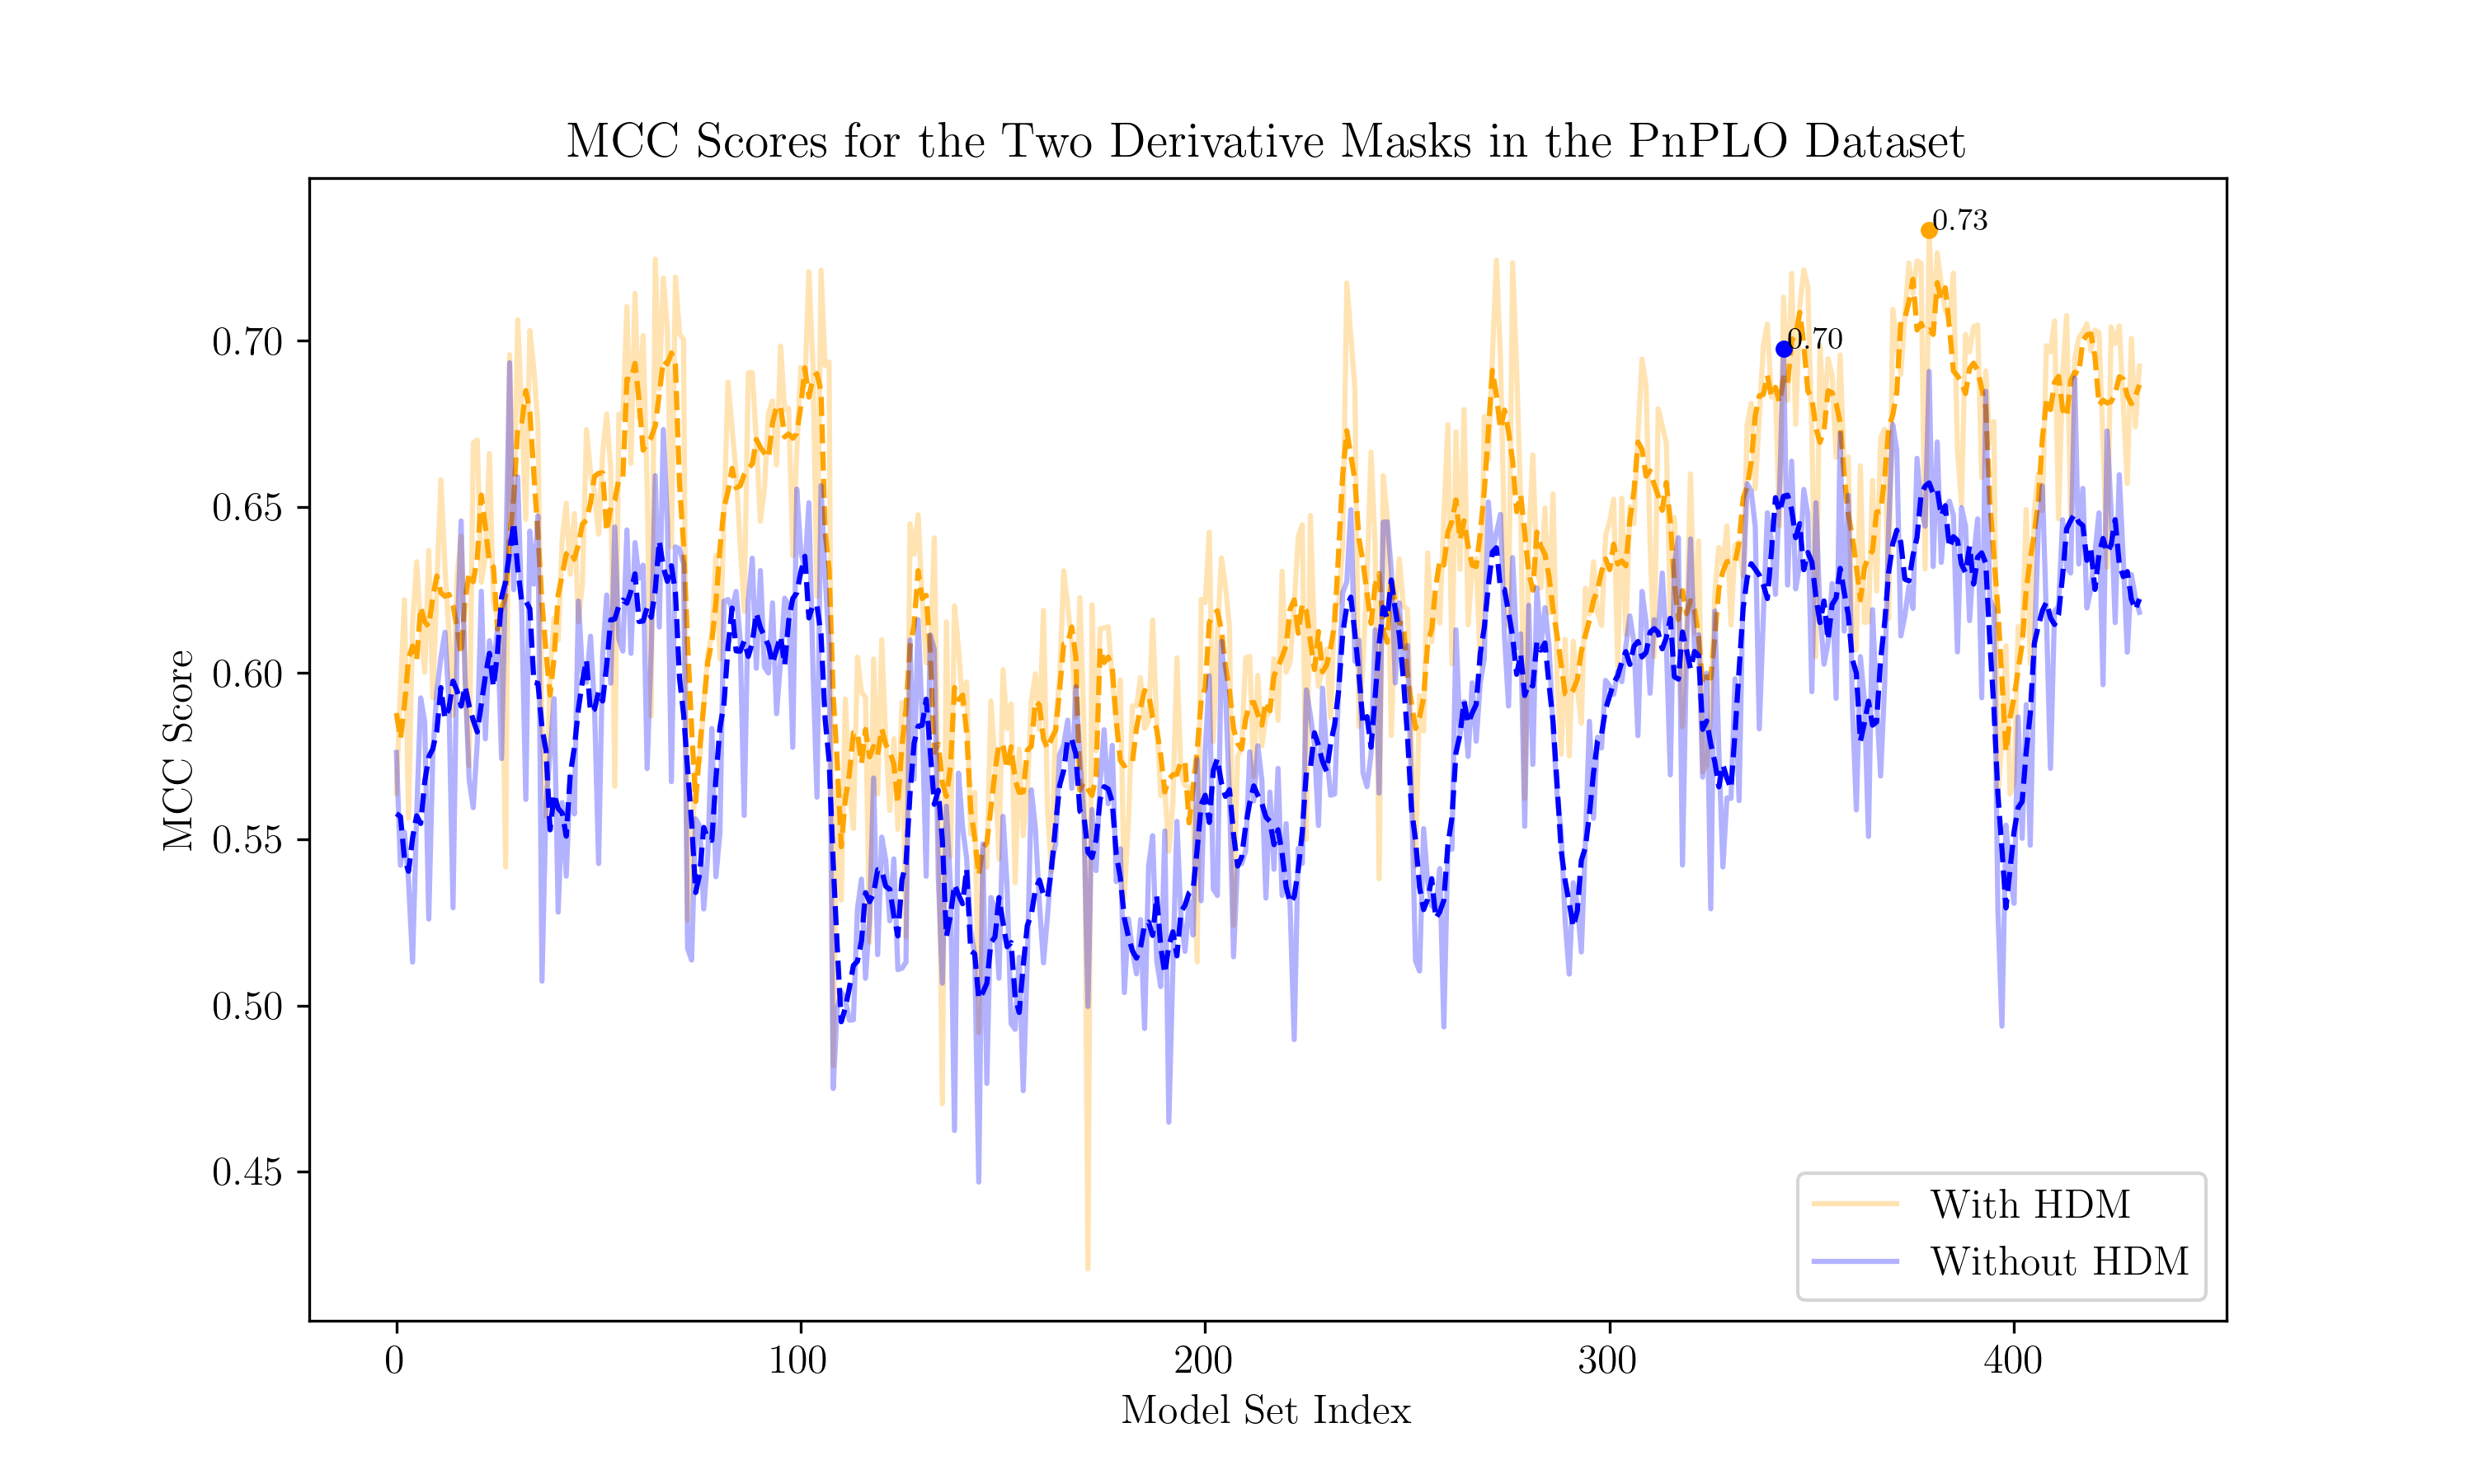
\includegraphics[width=0.9\linewidth]{mcc_hdm_PnPLO.png}
    \caption{
        MCC scores for PnPLO dataset, grouped by derivative mask. HDM stands for holistic derivative mask, as introduced in section \ref{sec:deriv_mask}.
    }
    \label{fig:hdm_pnplo}
\end{figure}

\begin{figure}
    \centering
    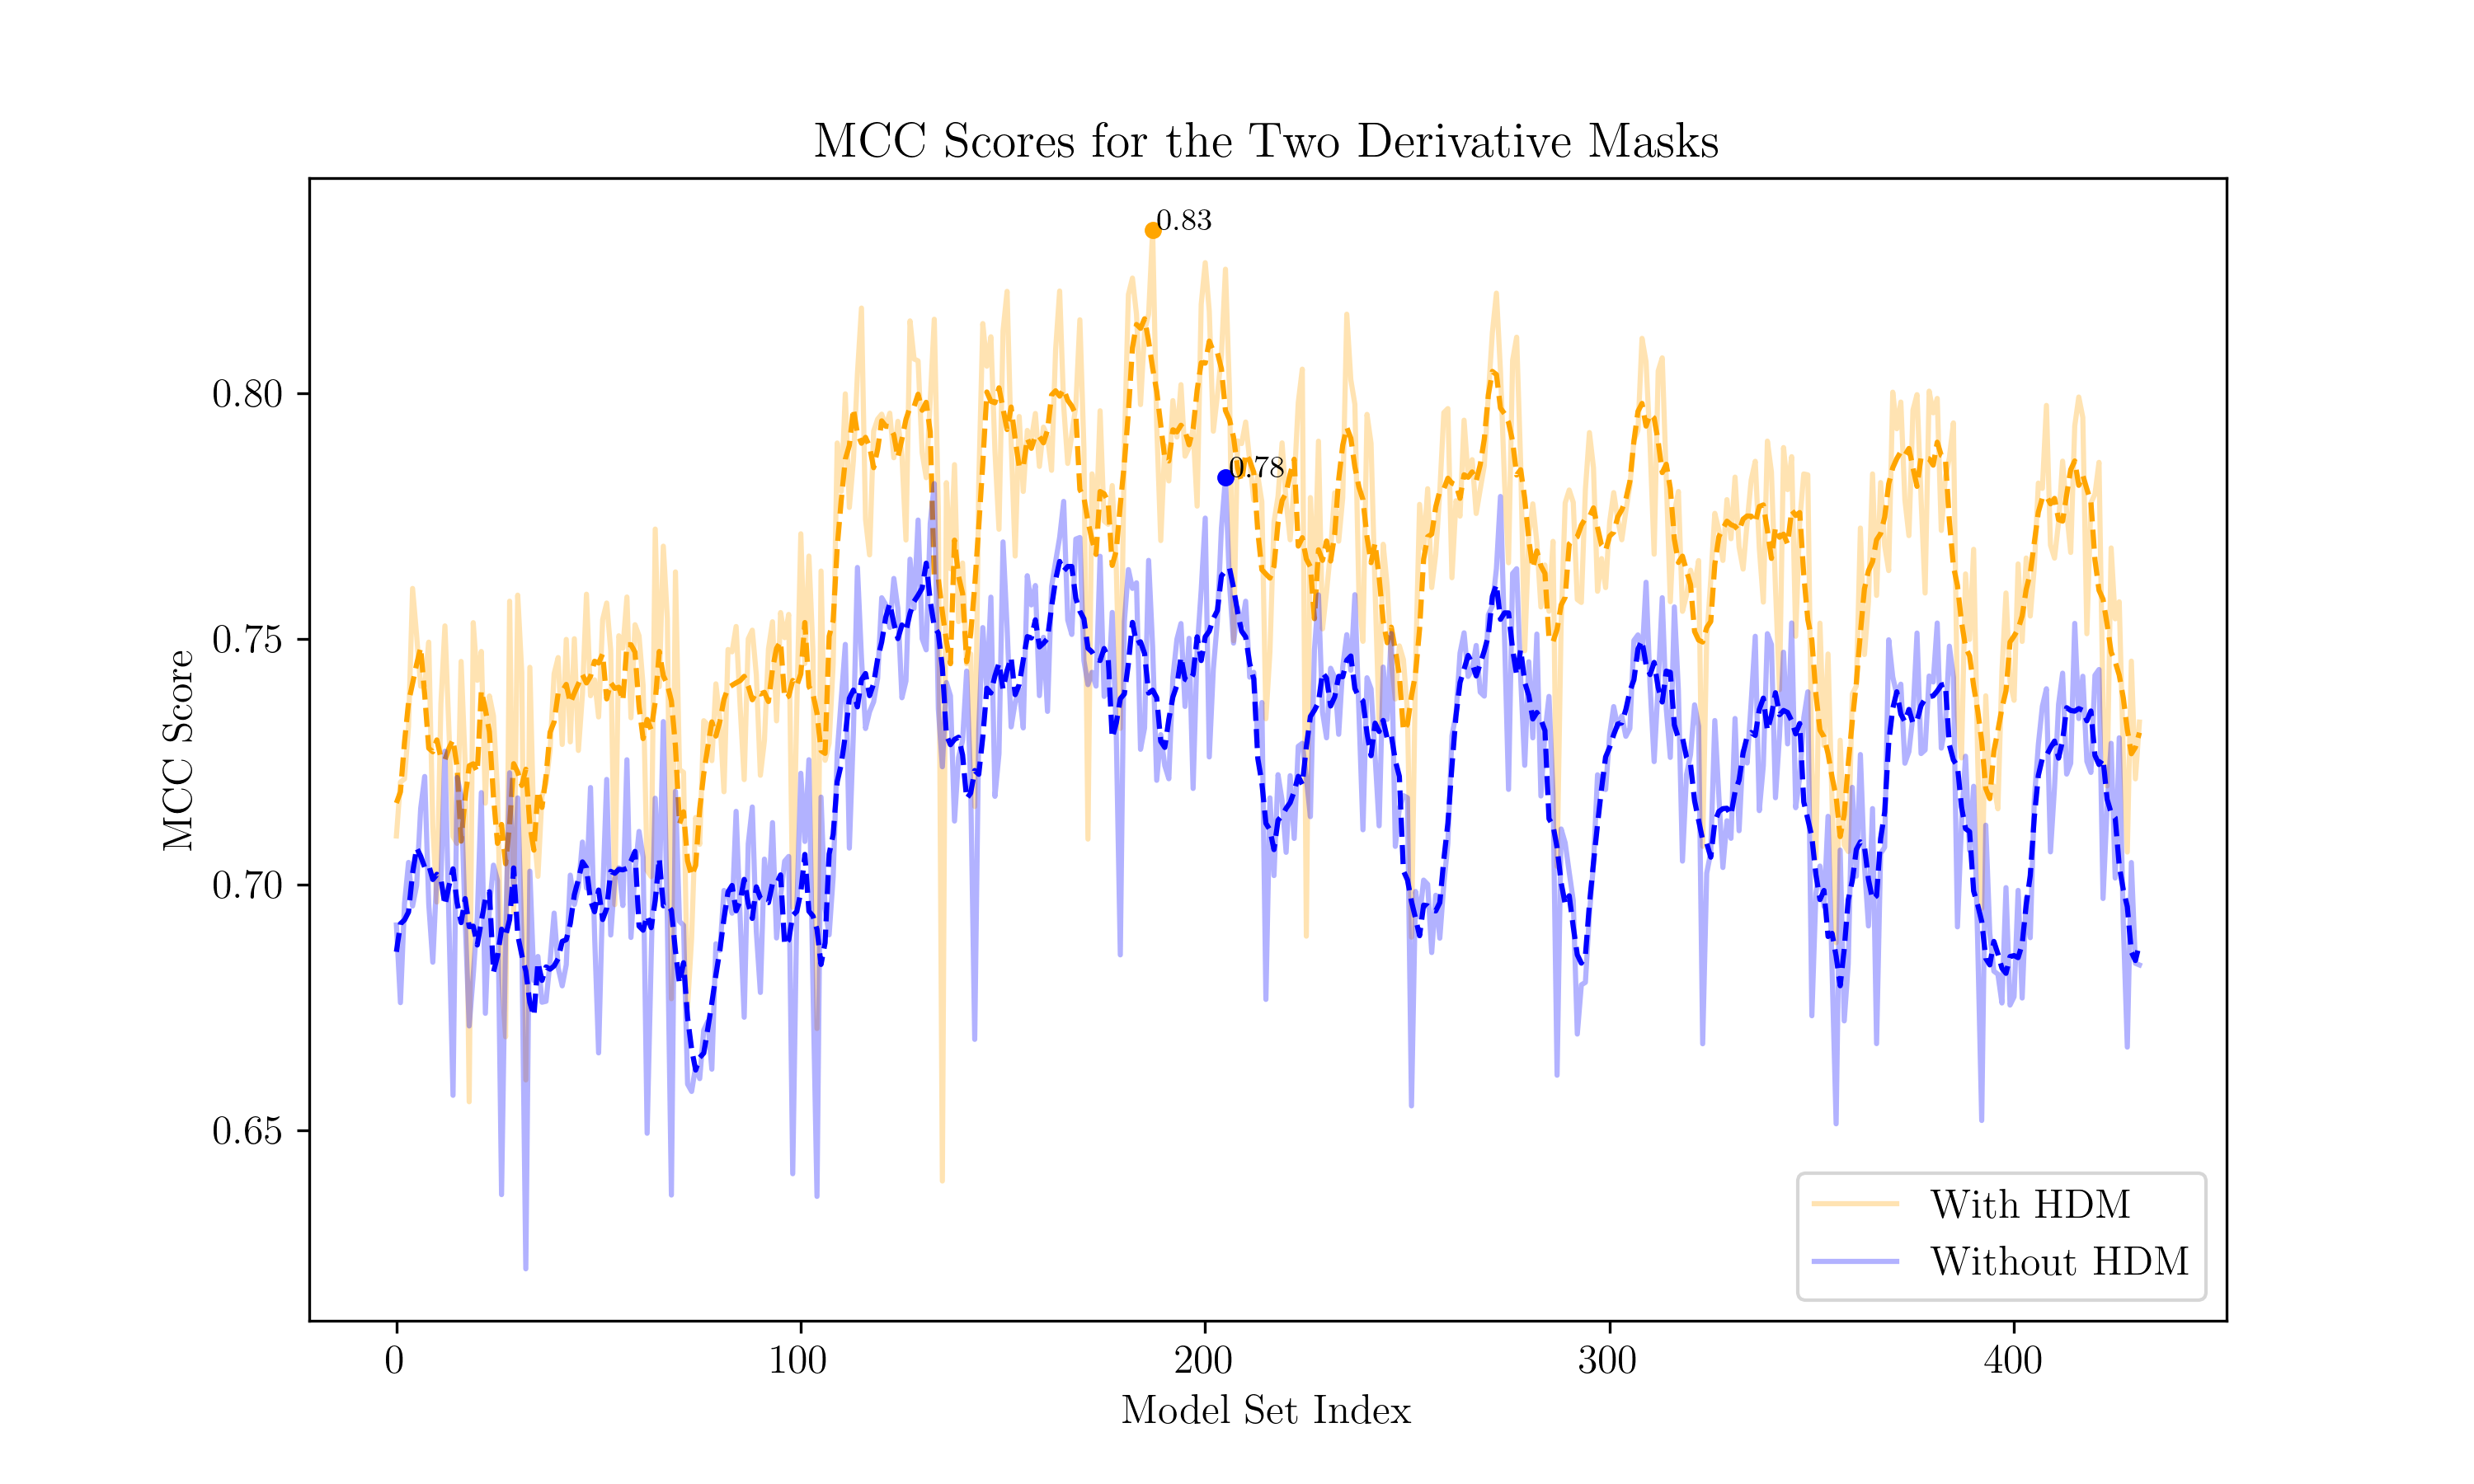
\includegraphics[width=0.9\linewidth]{mcc_hdm_total.png}
    \caption{
        MCC scores for the aggregate test dataset, grouped by derivative mask. HDM stands for holistic derivative mask, as introduced in section \ref{sec:deriv_mask}.
    }
    \label{fig:hdm_total}
\end{figure}


\subsubsection{Graphs for Different Orientation Bin Sizes}

\begin{figure}
    \centering
    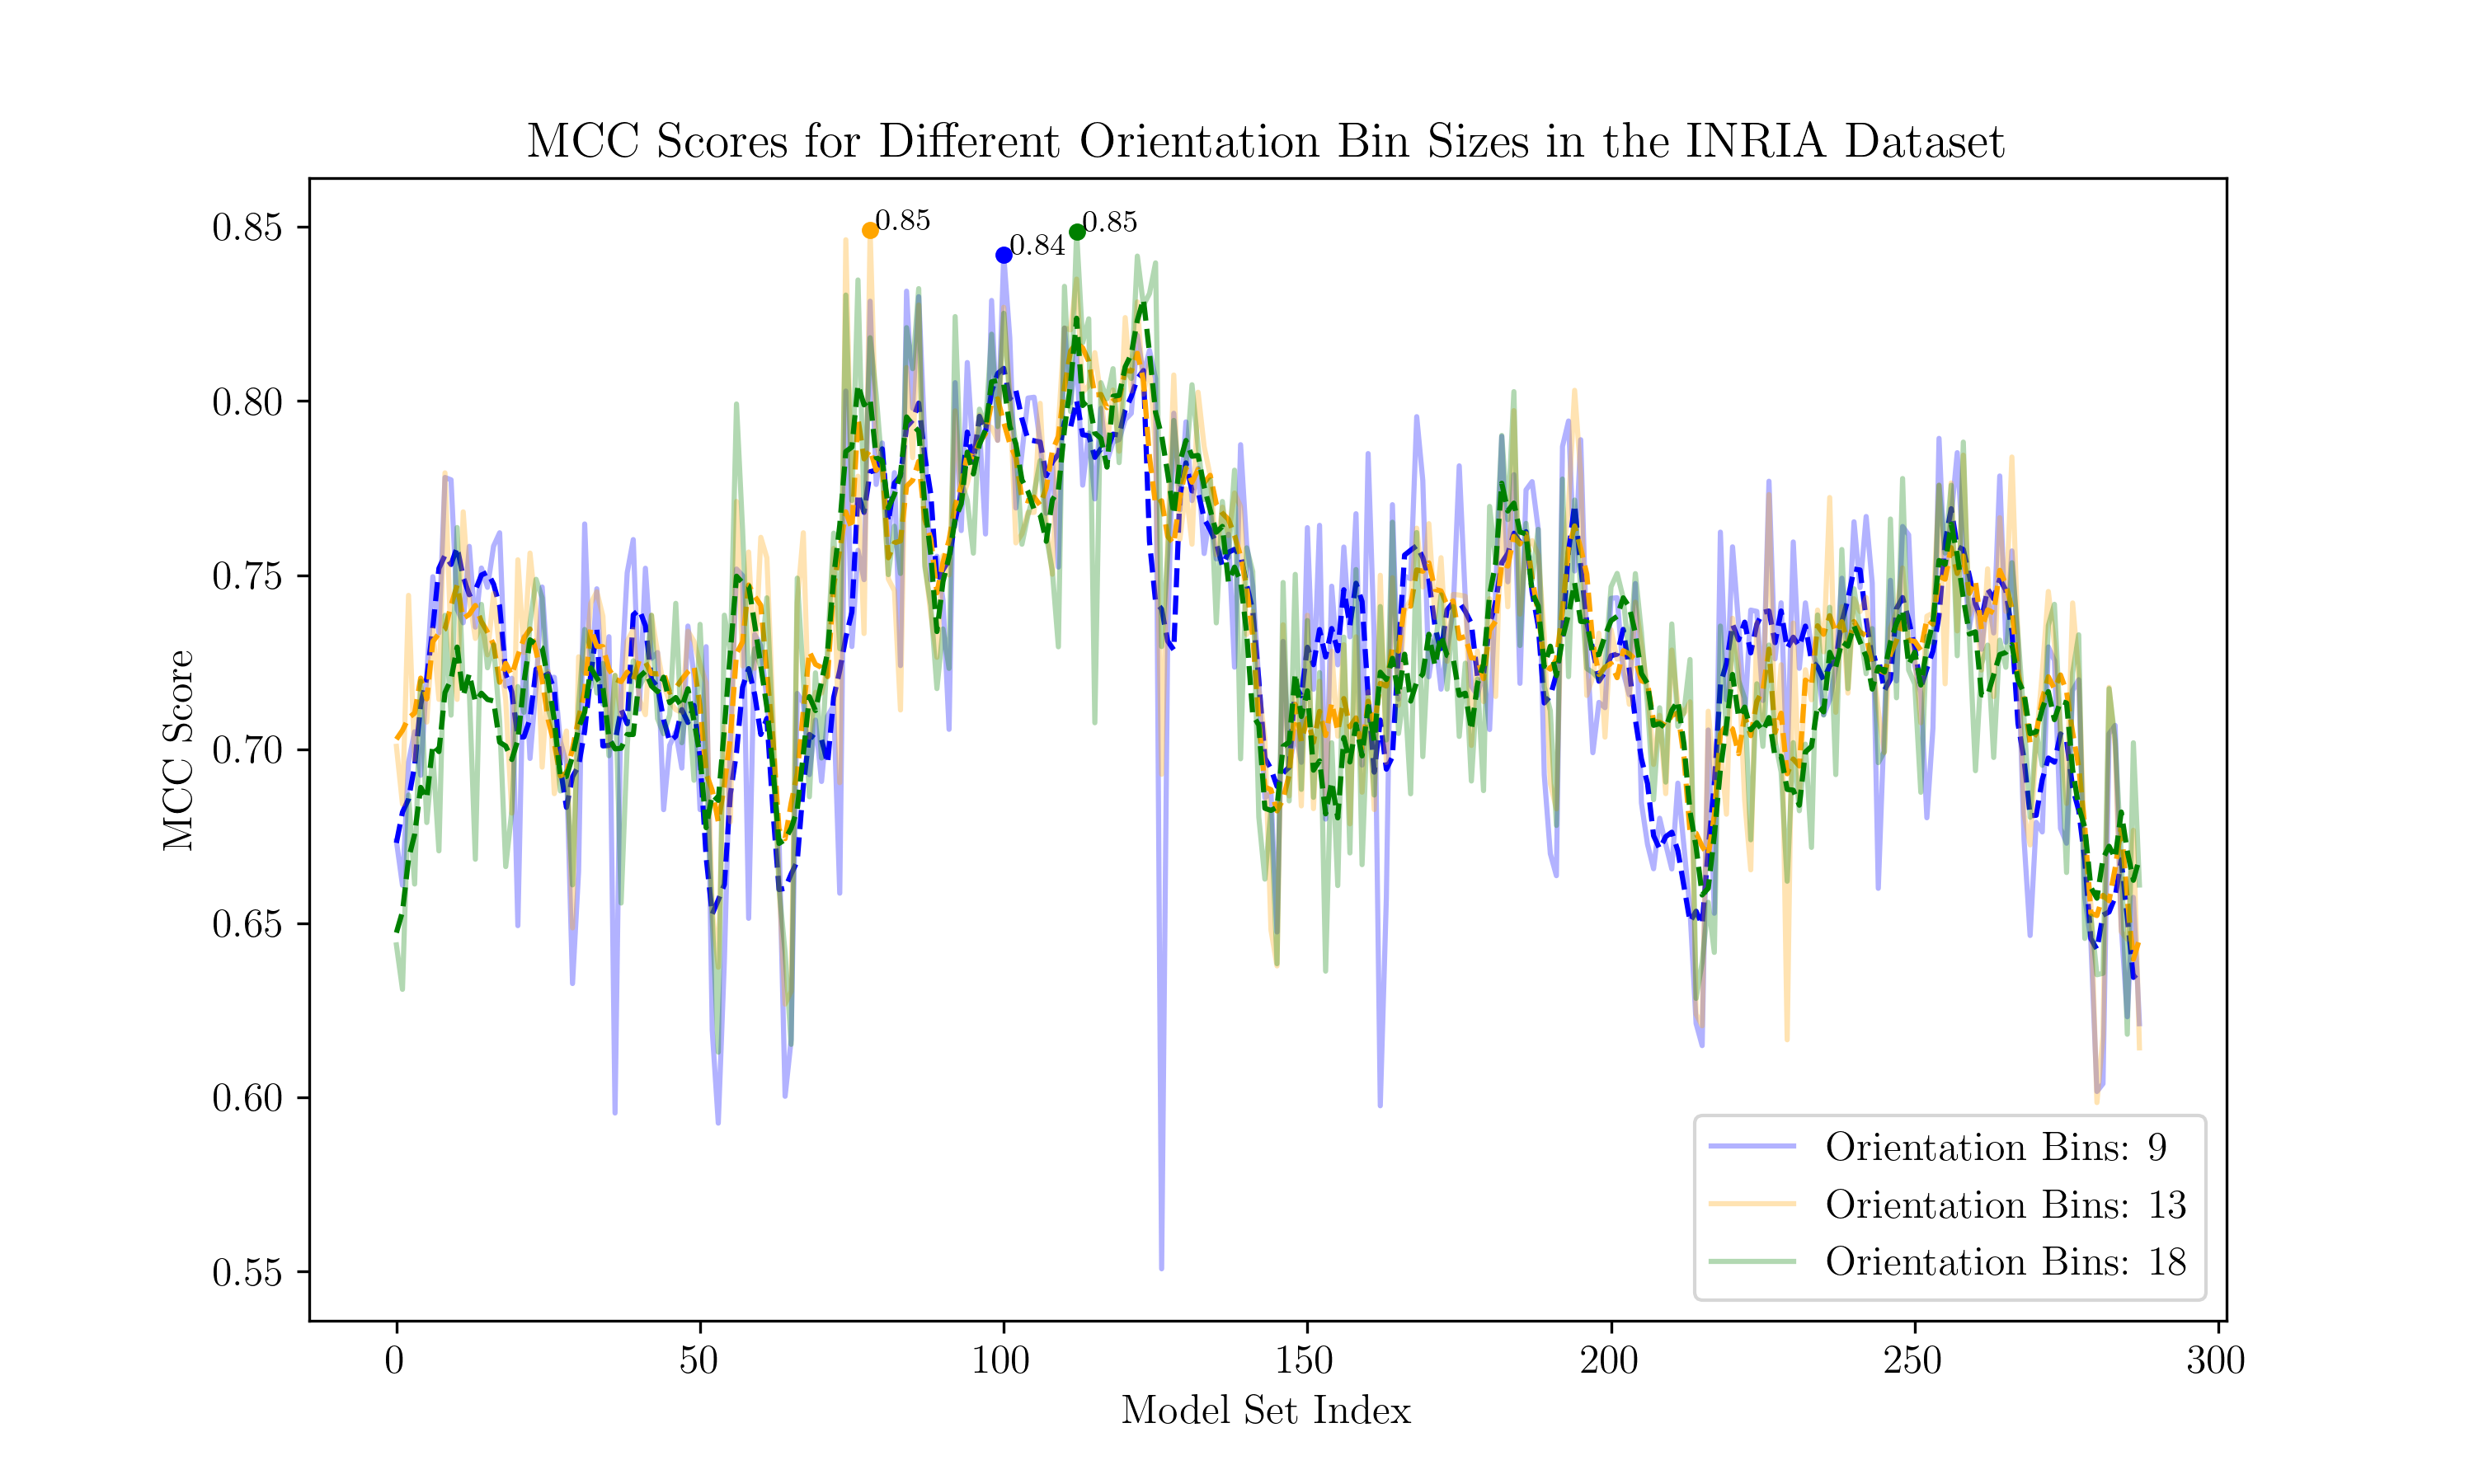
\includegraphics[width=0.9\linewidth]{mcc_bins_INRIA.png}
    \caption{
        MCC scores for INRIA dataset, grouped by orientation bin size.
    }
    \label{fig:orientation_bins_inria}
\end{figure}

\begin{figure}
    \centering
    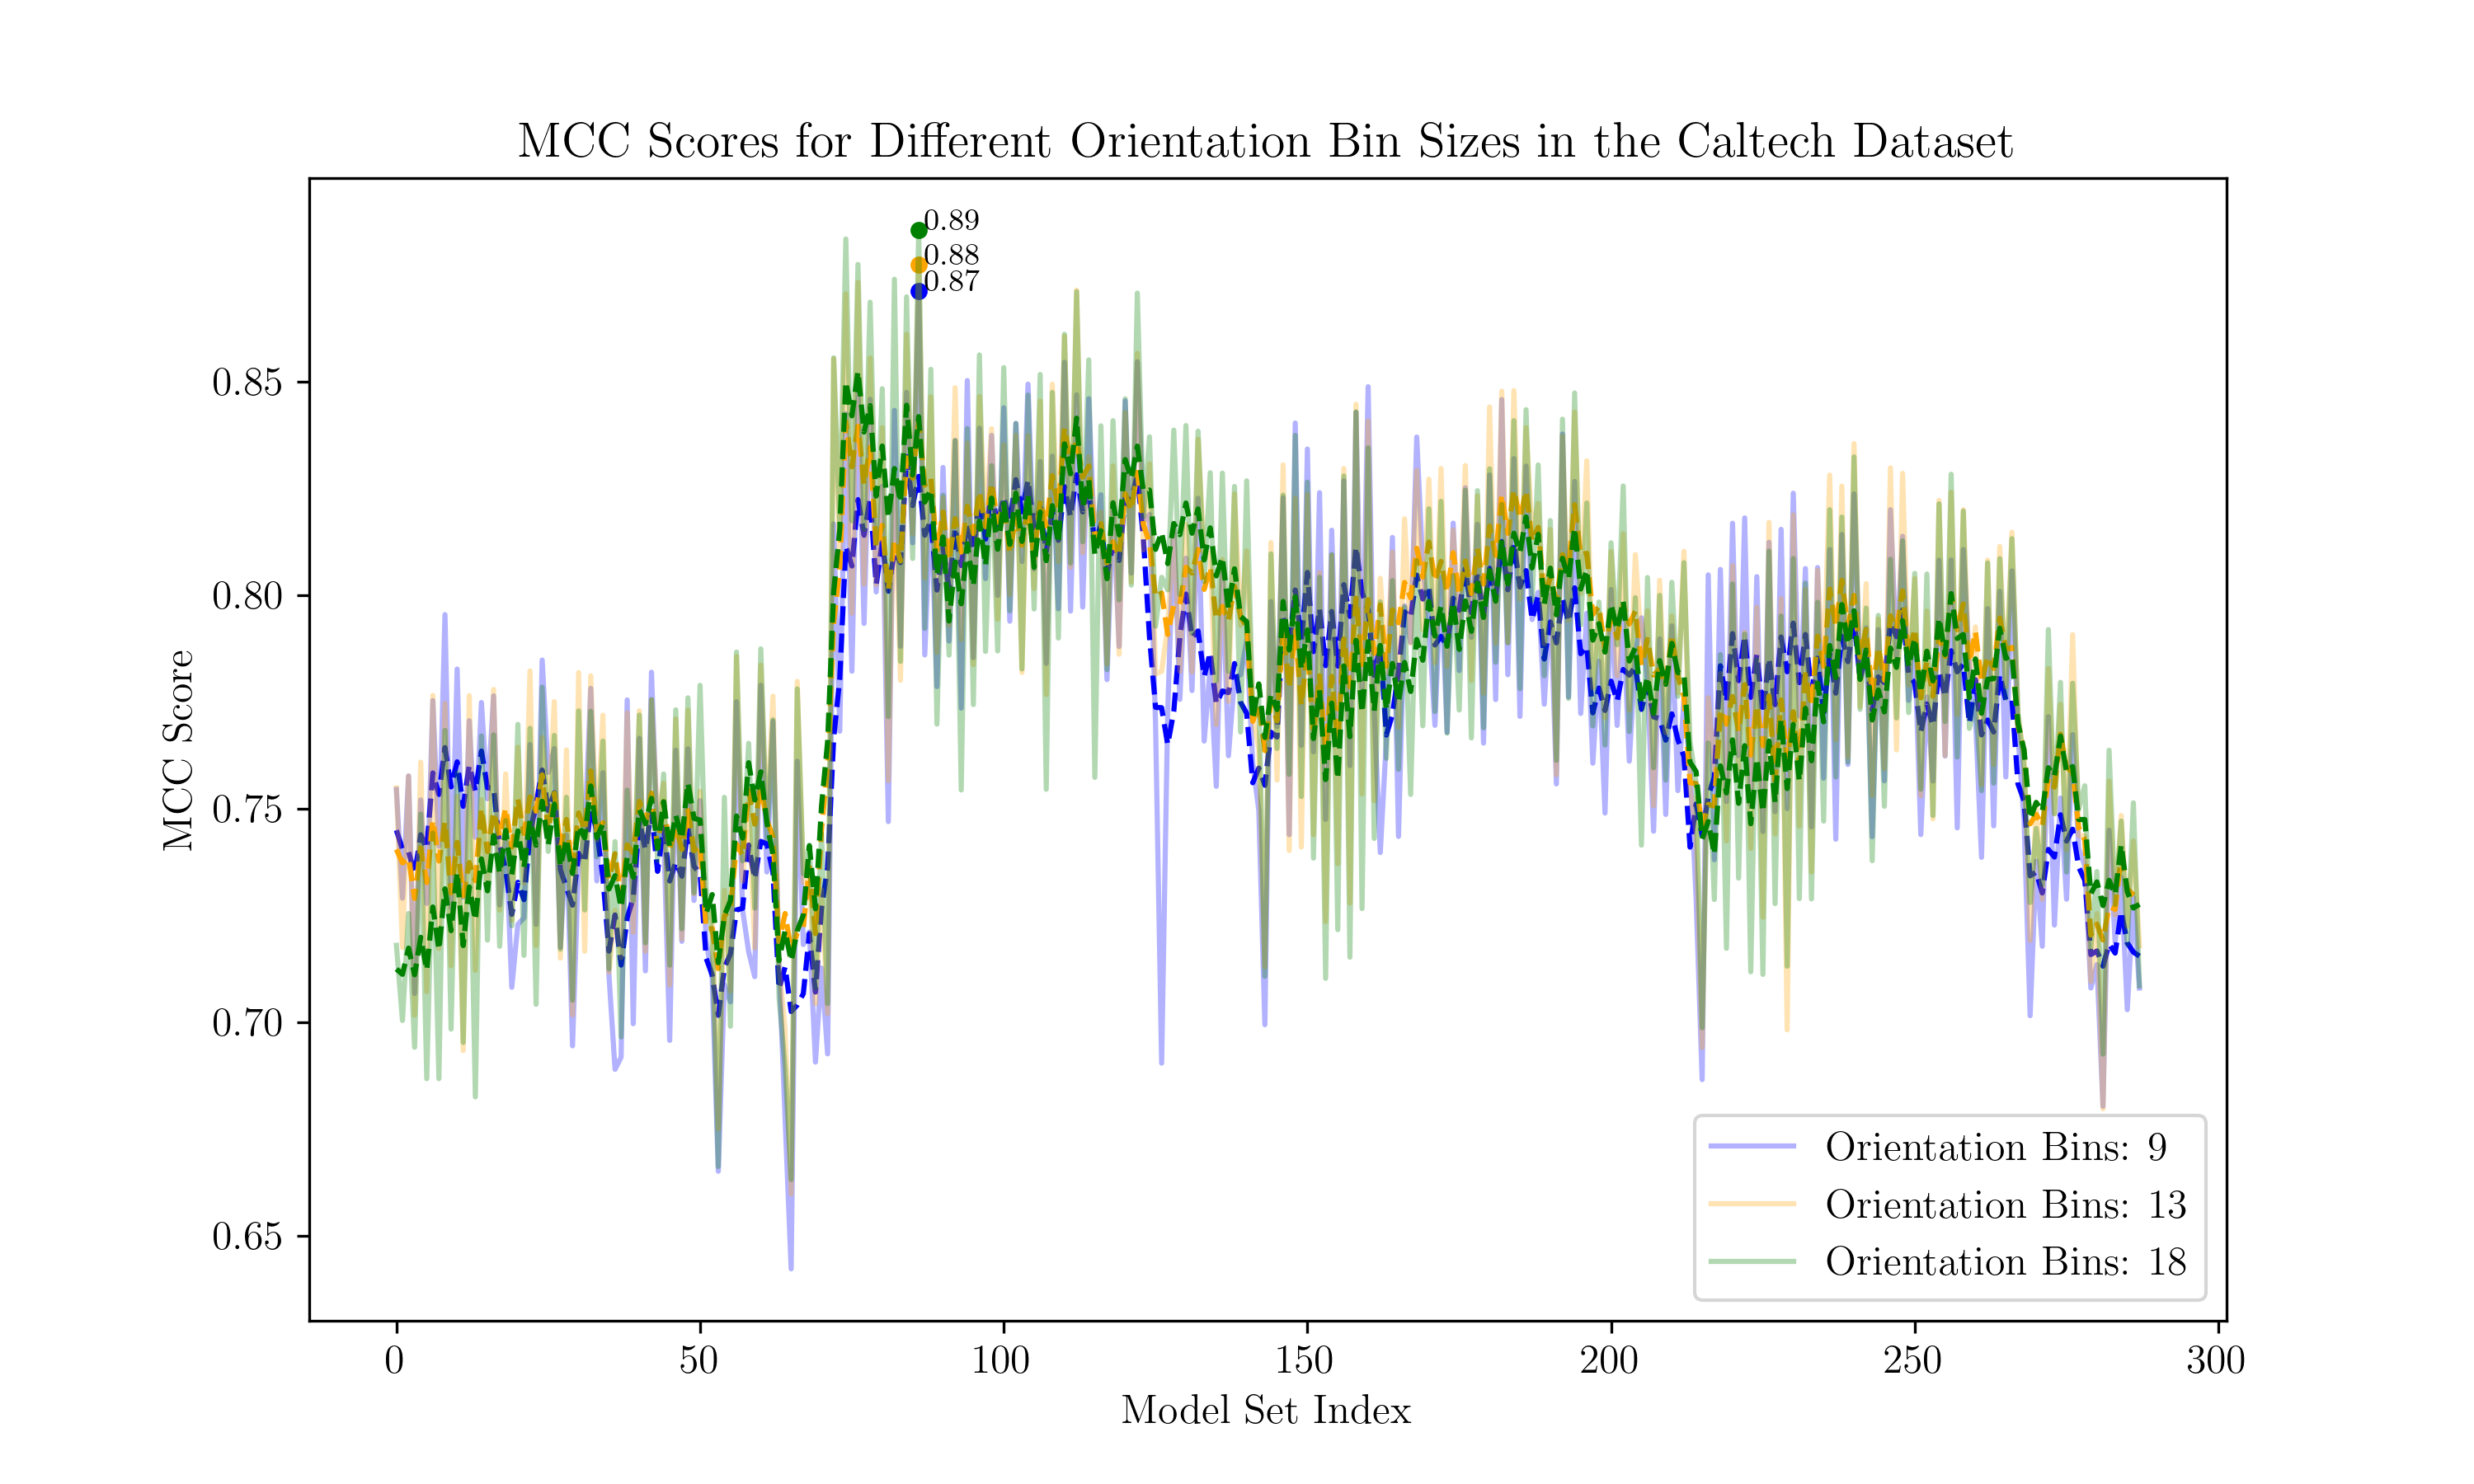
\includegraphics[width=0.9\linewidth]{mcc_bins_caltech_30.png}
    \caption{
        MCC scores for Caltech dataset, grouped by orientation bin size.
    }
\end{figure}

\begin{figure}
    \centering
    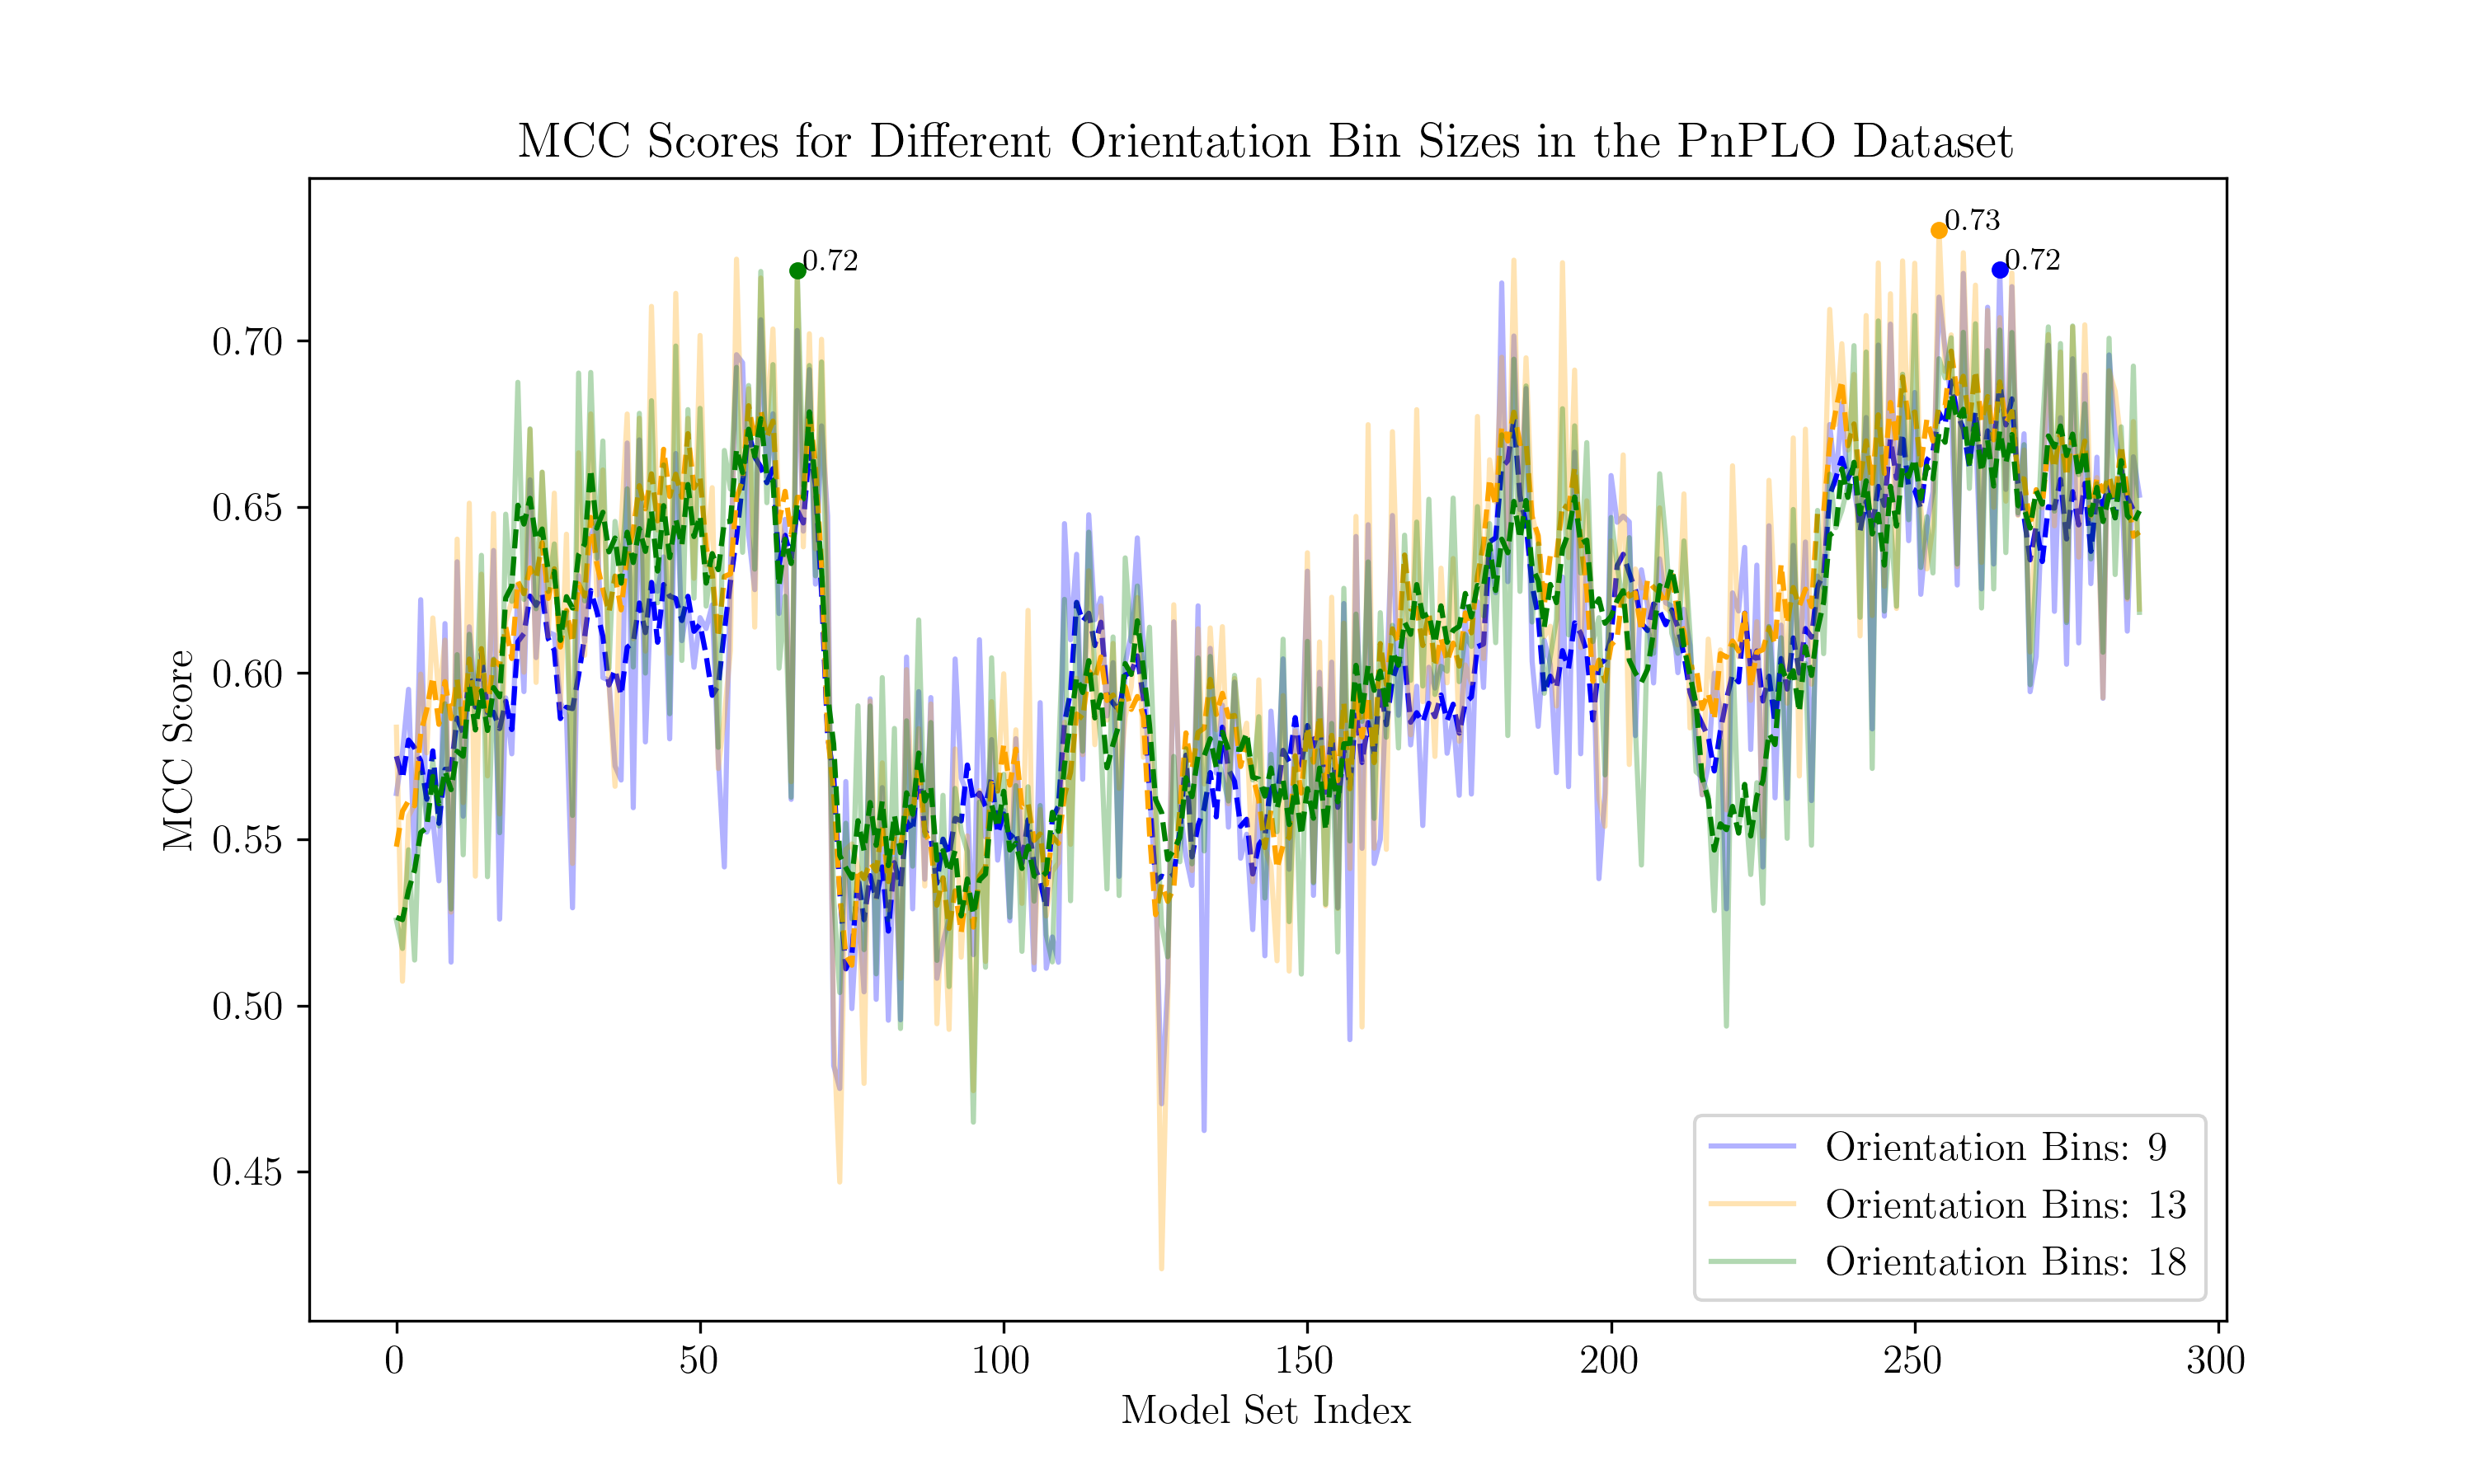
\includegraphics[width=0.9\linewidth]{mcc_bins_PnPLO.png}
    \caption{
        MCC scores for PnPLO dataset, grouped by orientation bin size.
    }
\end{figure}

\begin{figure}
    \centering
    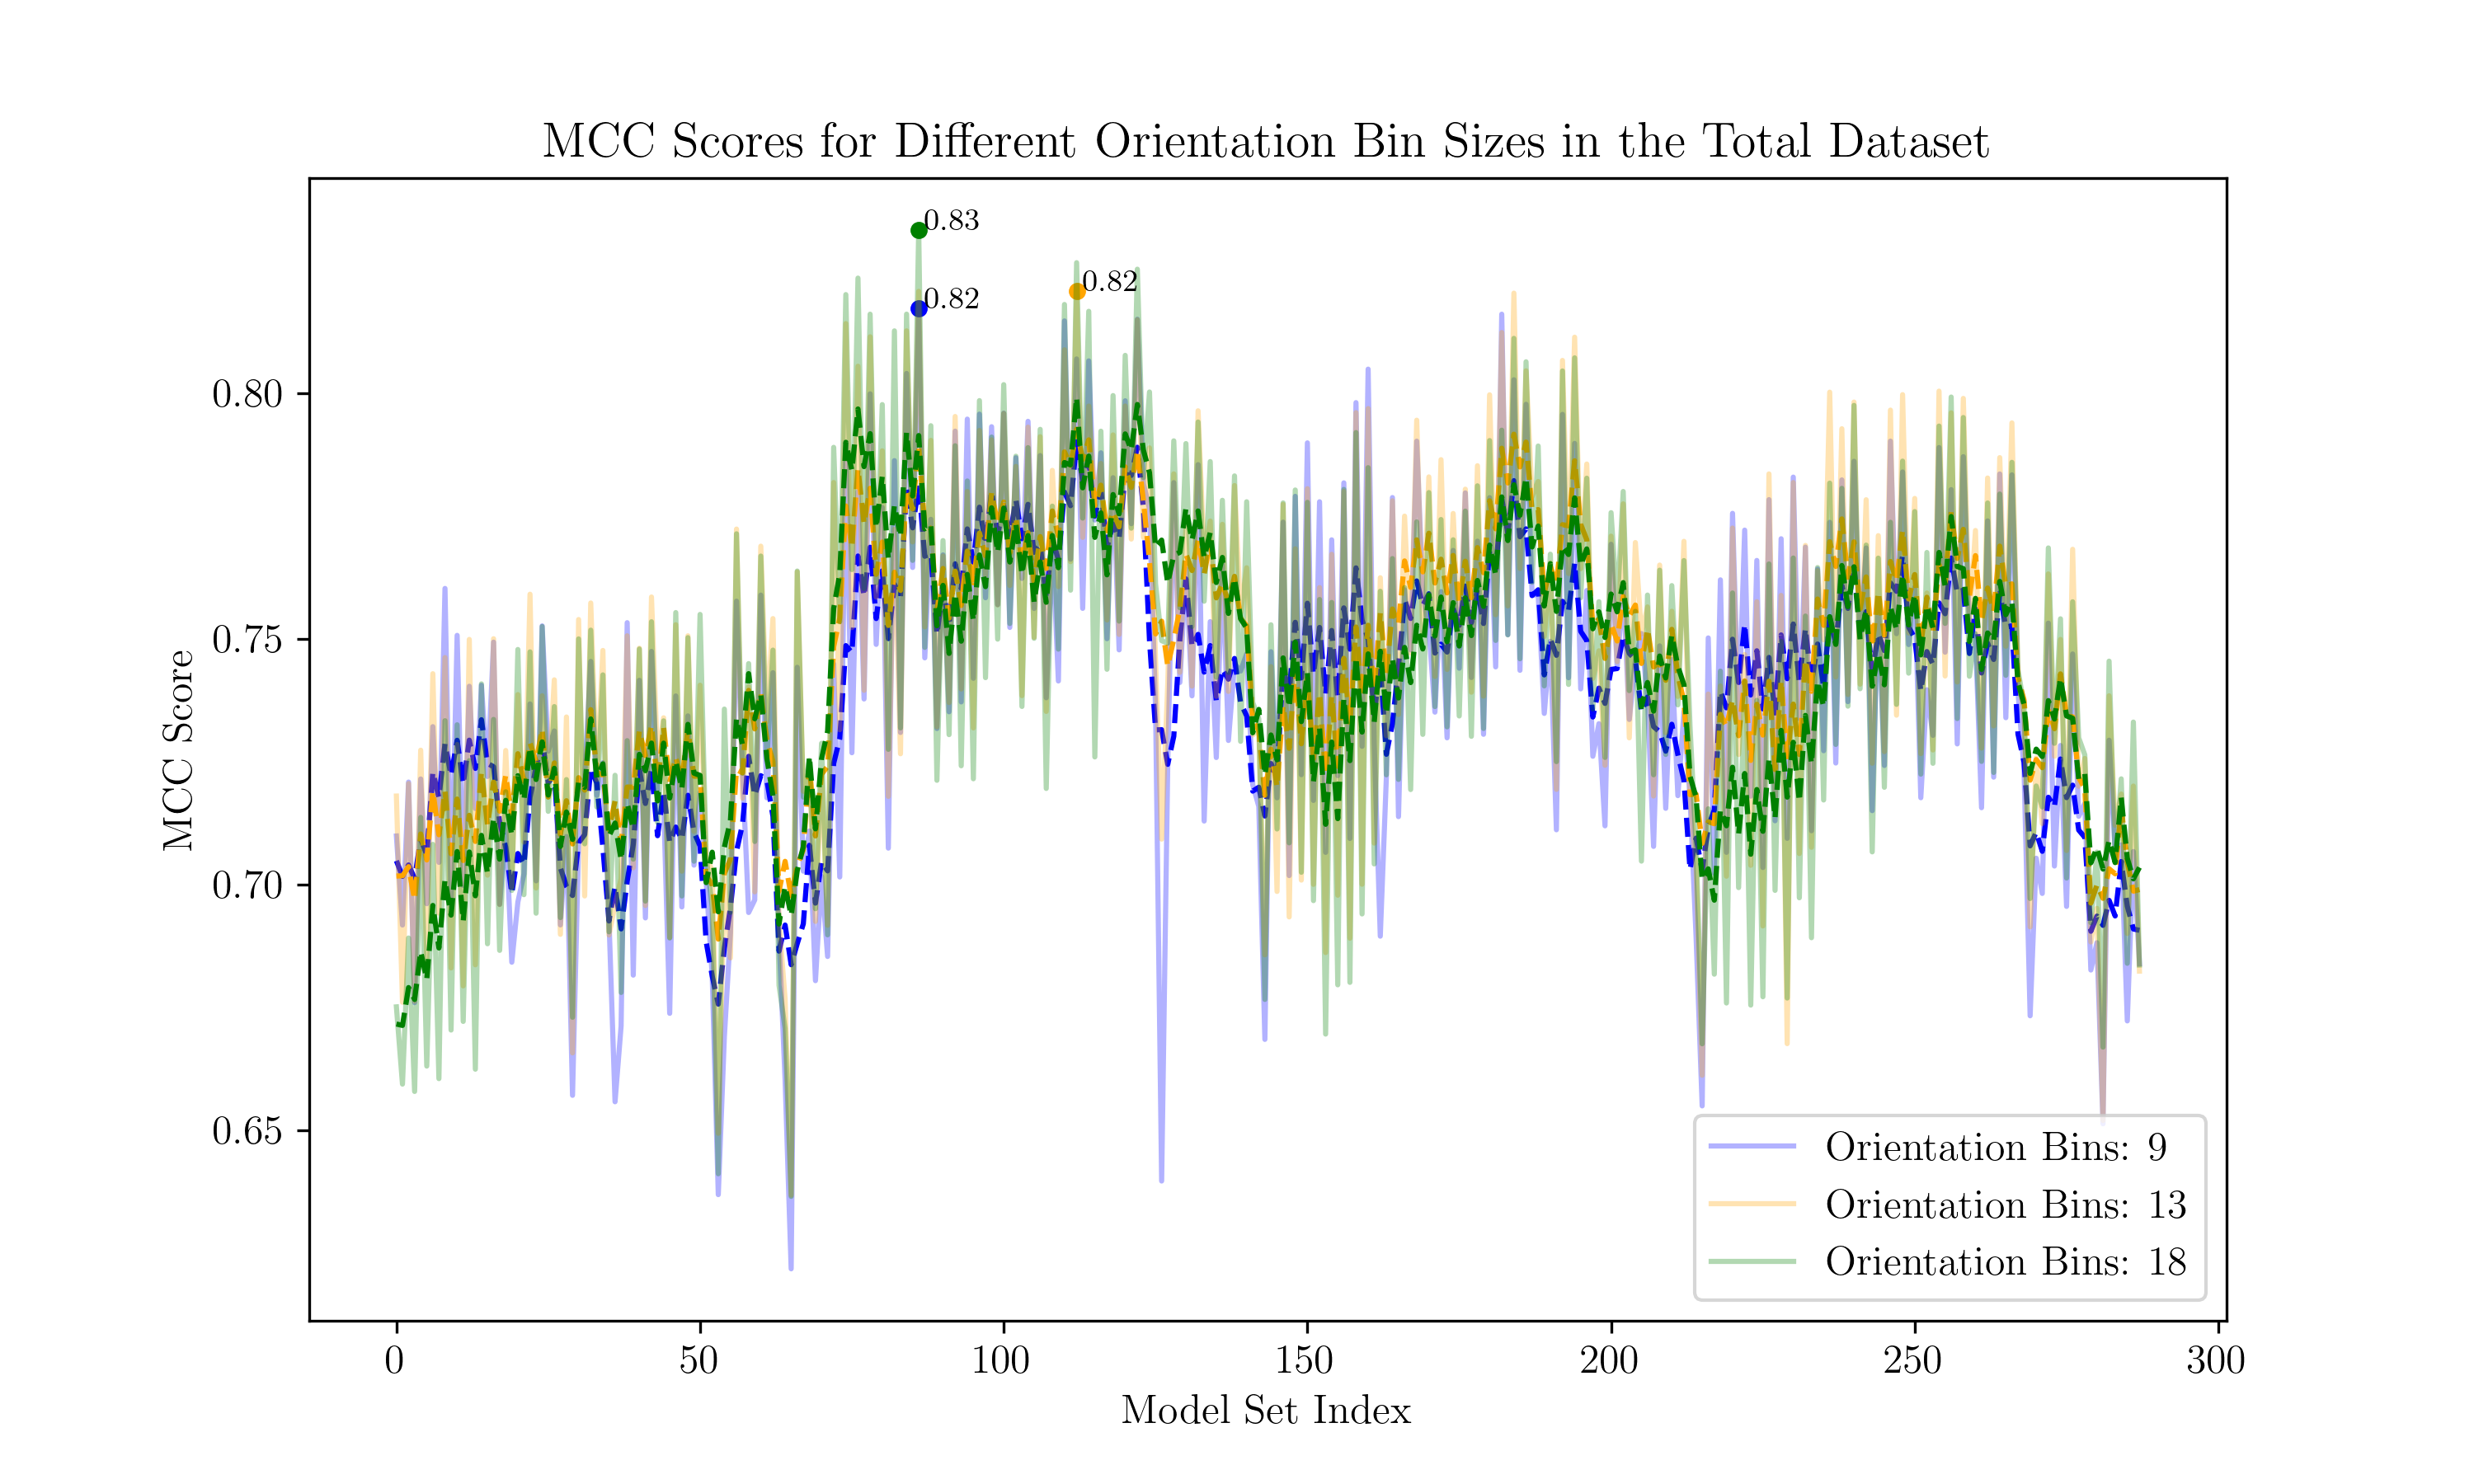
\includegraphics[width=0.9\linewidth]{mcc_bins_total.png}
    \caption{
        MCC scores for the aggregate test dataset, grouped by orientation bin size.
    }
    \label{fig:orientation_bins_total}
\end{figure}


\subsubsection{Graphs and Heatmaps for Block Density}

Block density accurately describes the relationship between cell size and block size, though it's not commonly used in literature. Graphs that isolate either of the parameters fail to show their complex interactions, as seen in figures \ref{fig:cell_size_total} and \ref{fig:block_size_total}. Instead, a 2D matrix of block size and cell size with encoded MCC scores (a heatmap) better captures the relationship between the two parameters.

\begin{figure}
    \centering
    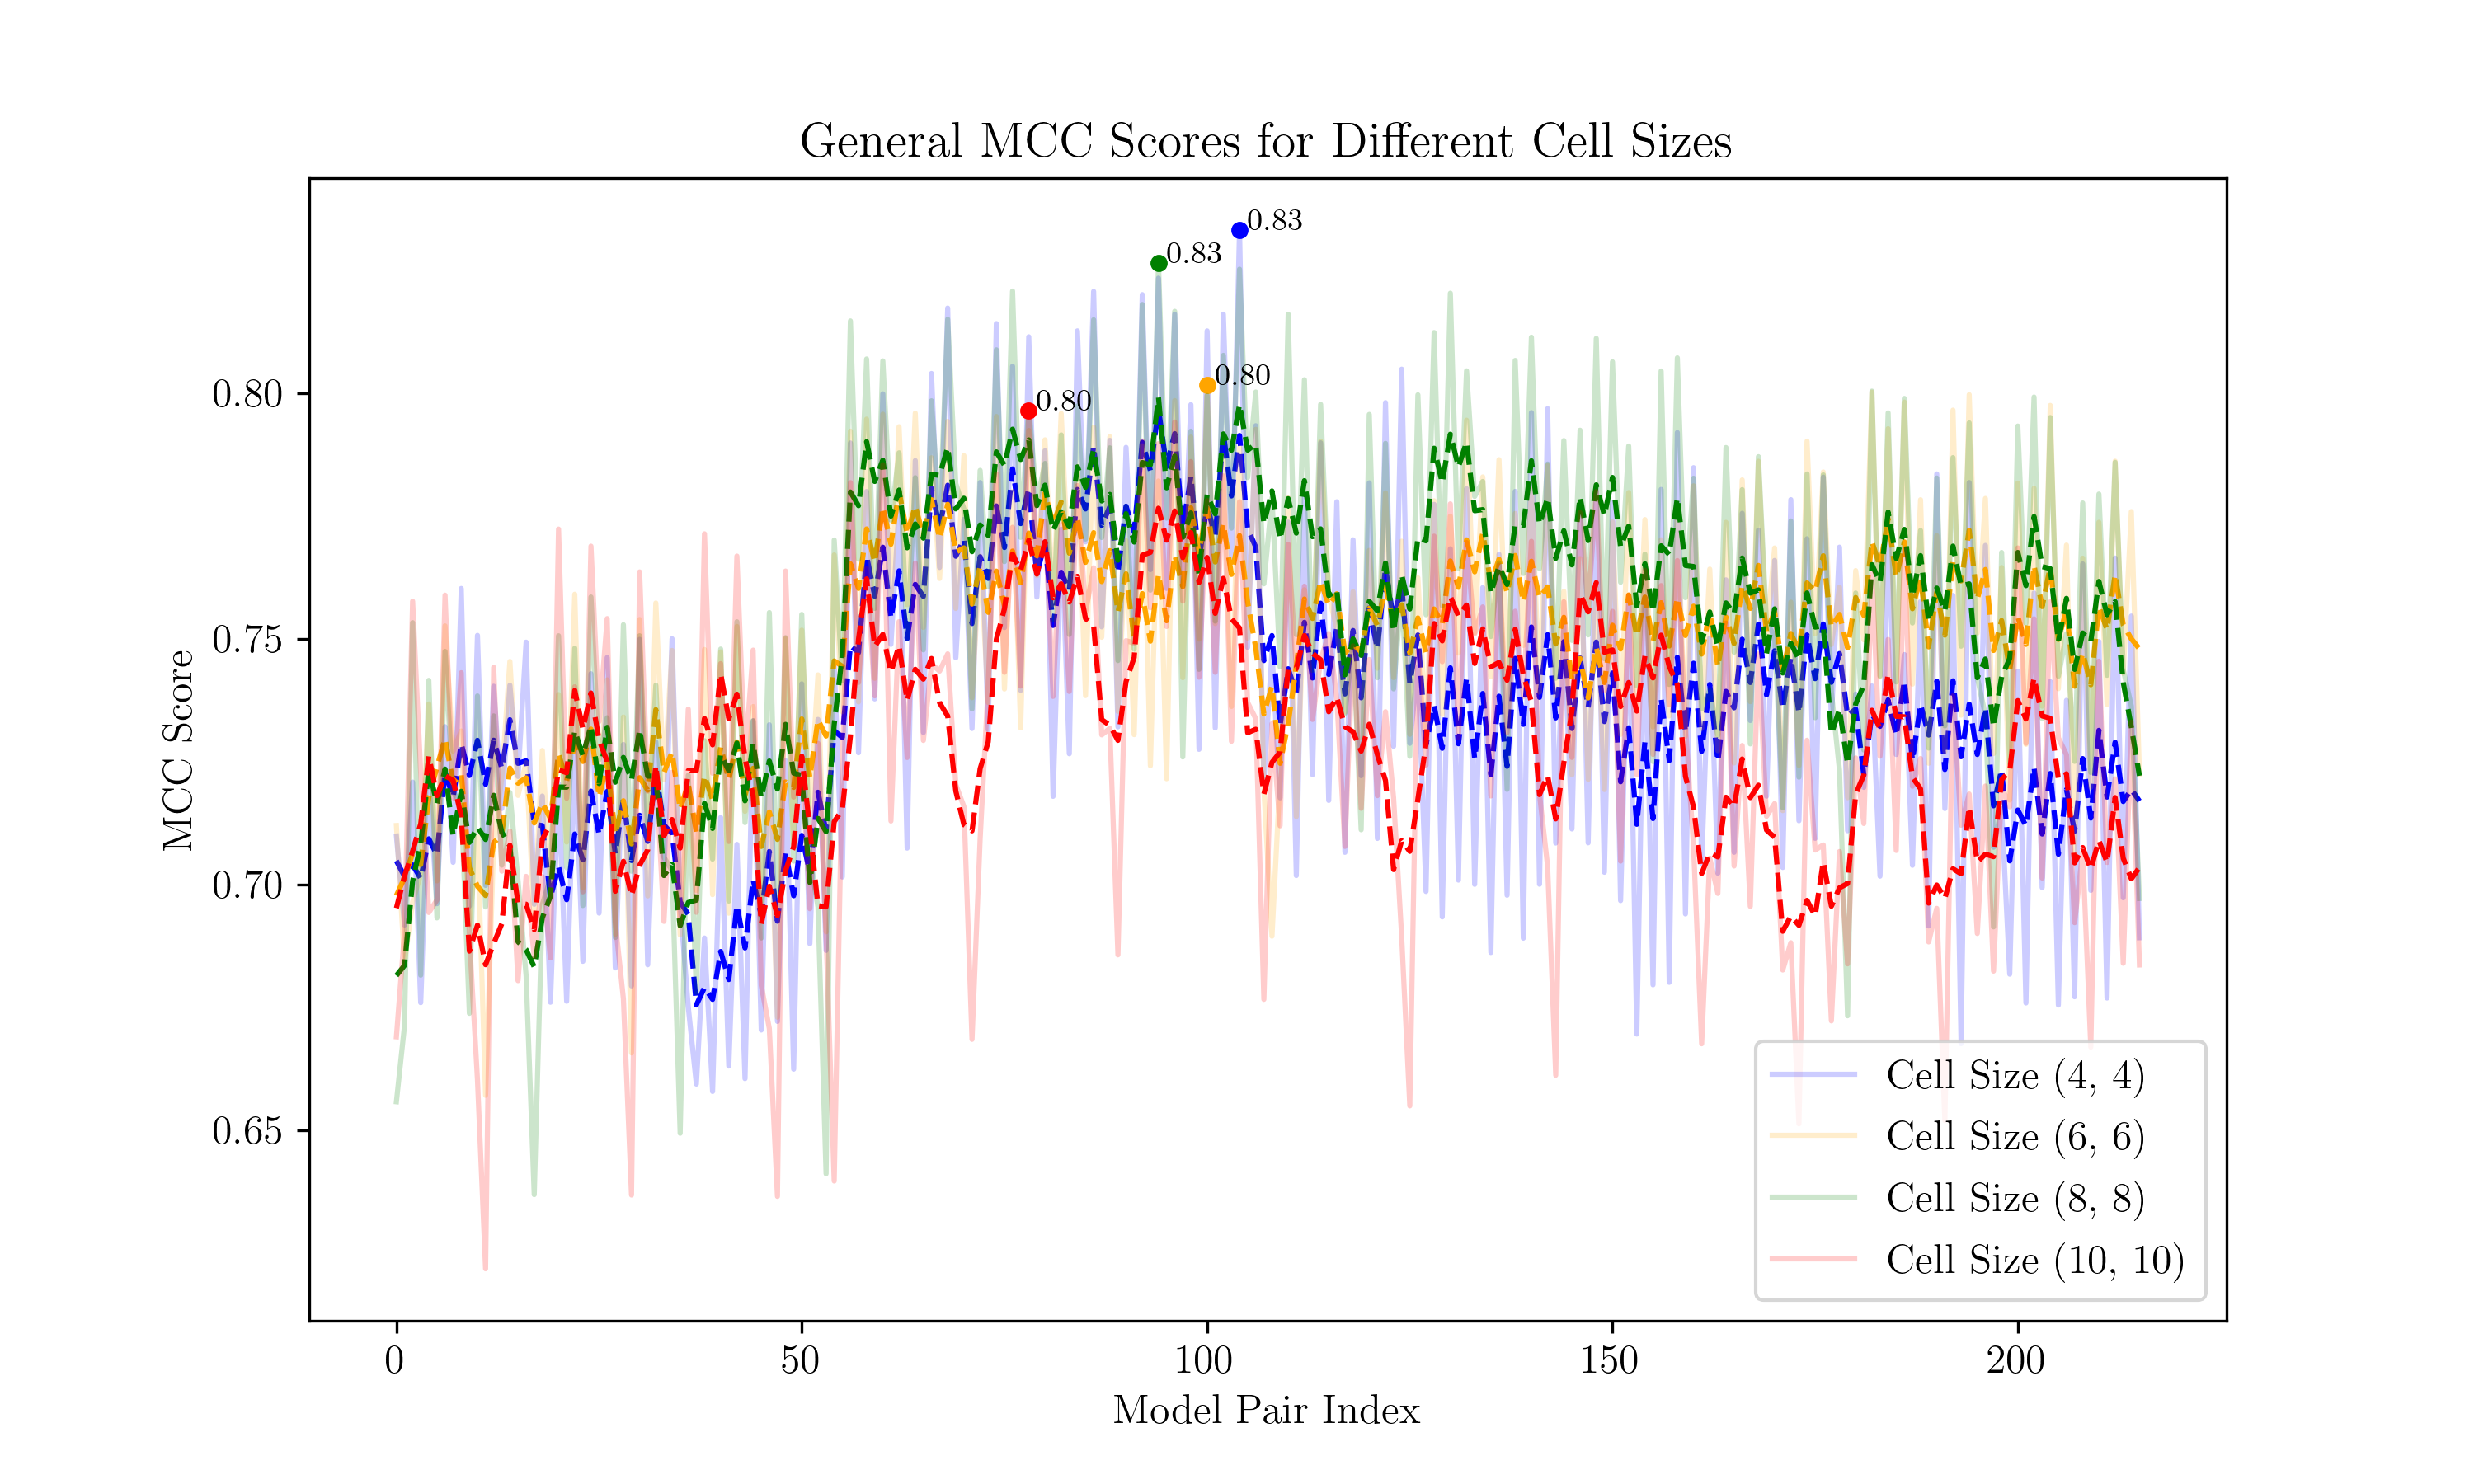
\includegraphics[width=0.9\linewidth]{mcc_cell_size_total.png}
    \caption{
        MCC scores for the aggregate test dataset, grouped by cell size.
    }
    \label{fig:cell_size_total}
\end{figure}

\begin{figure}
    \centering
    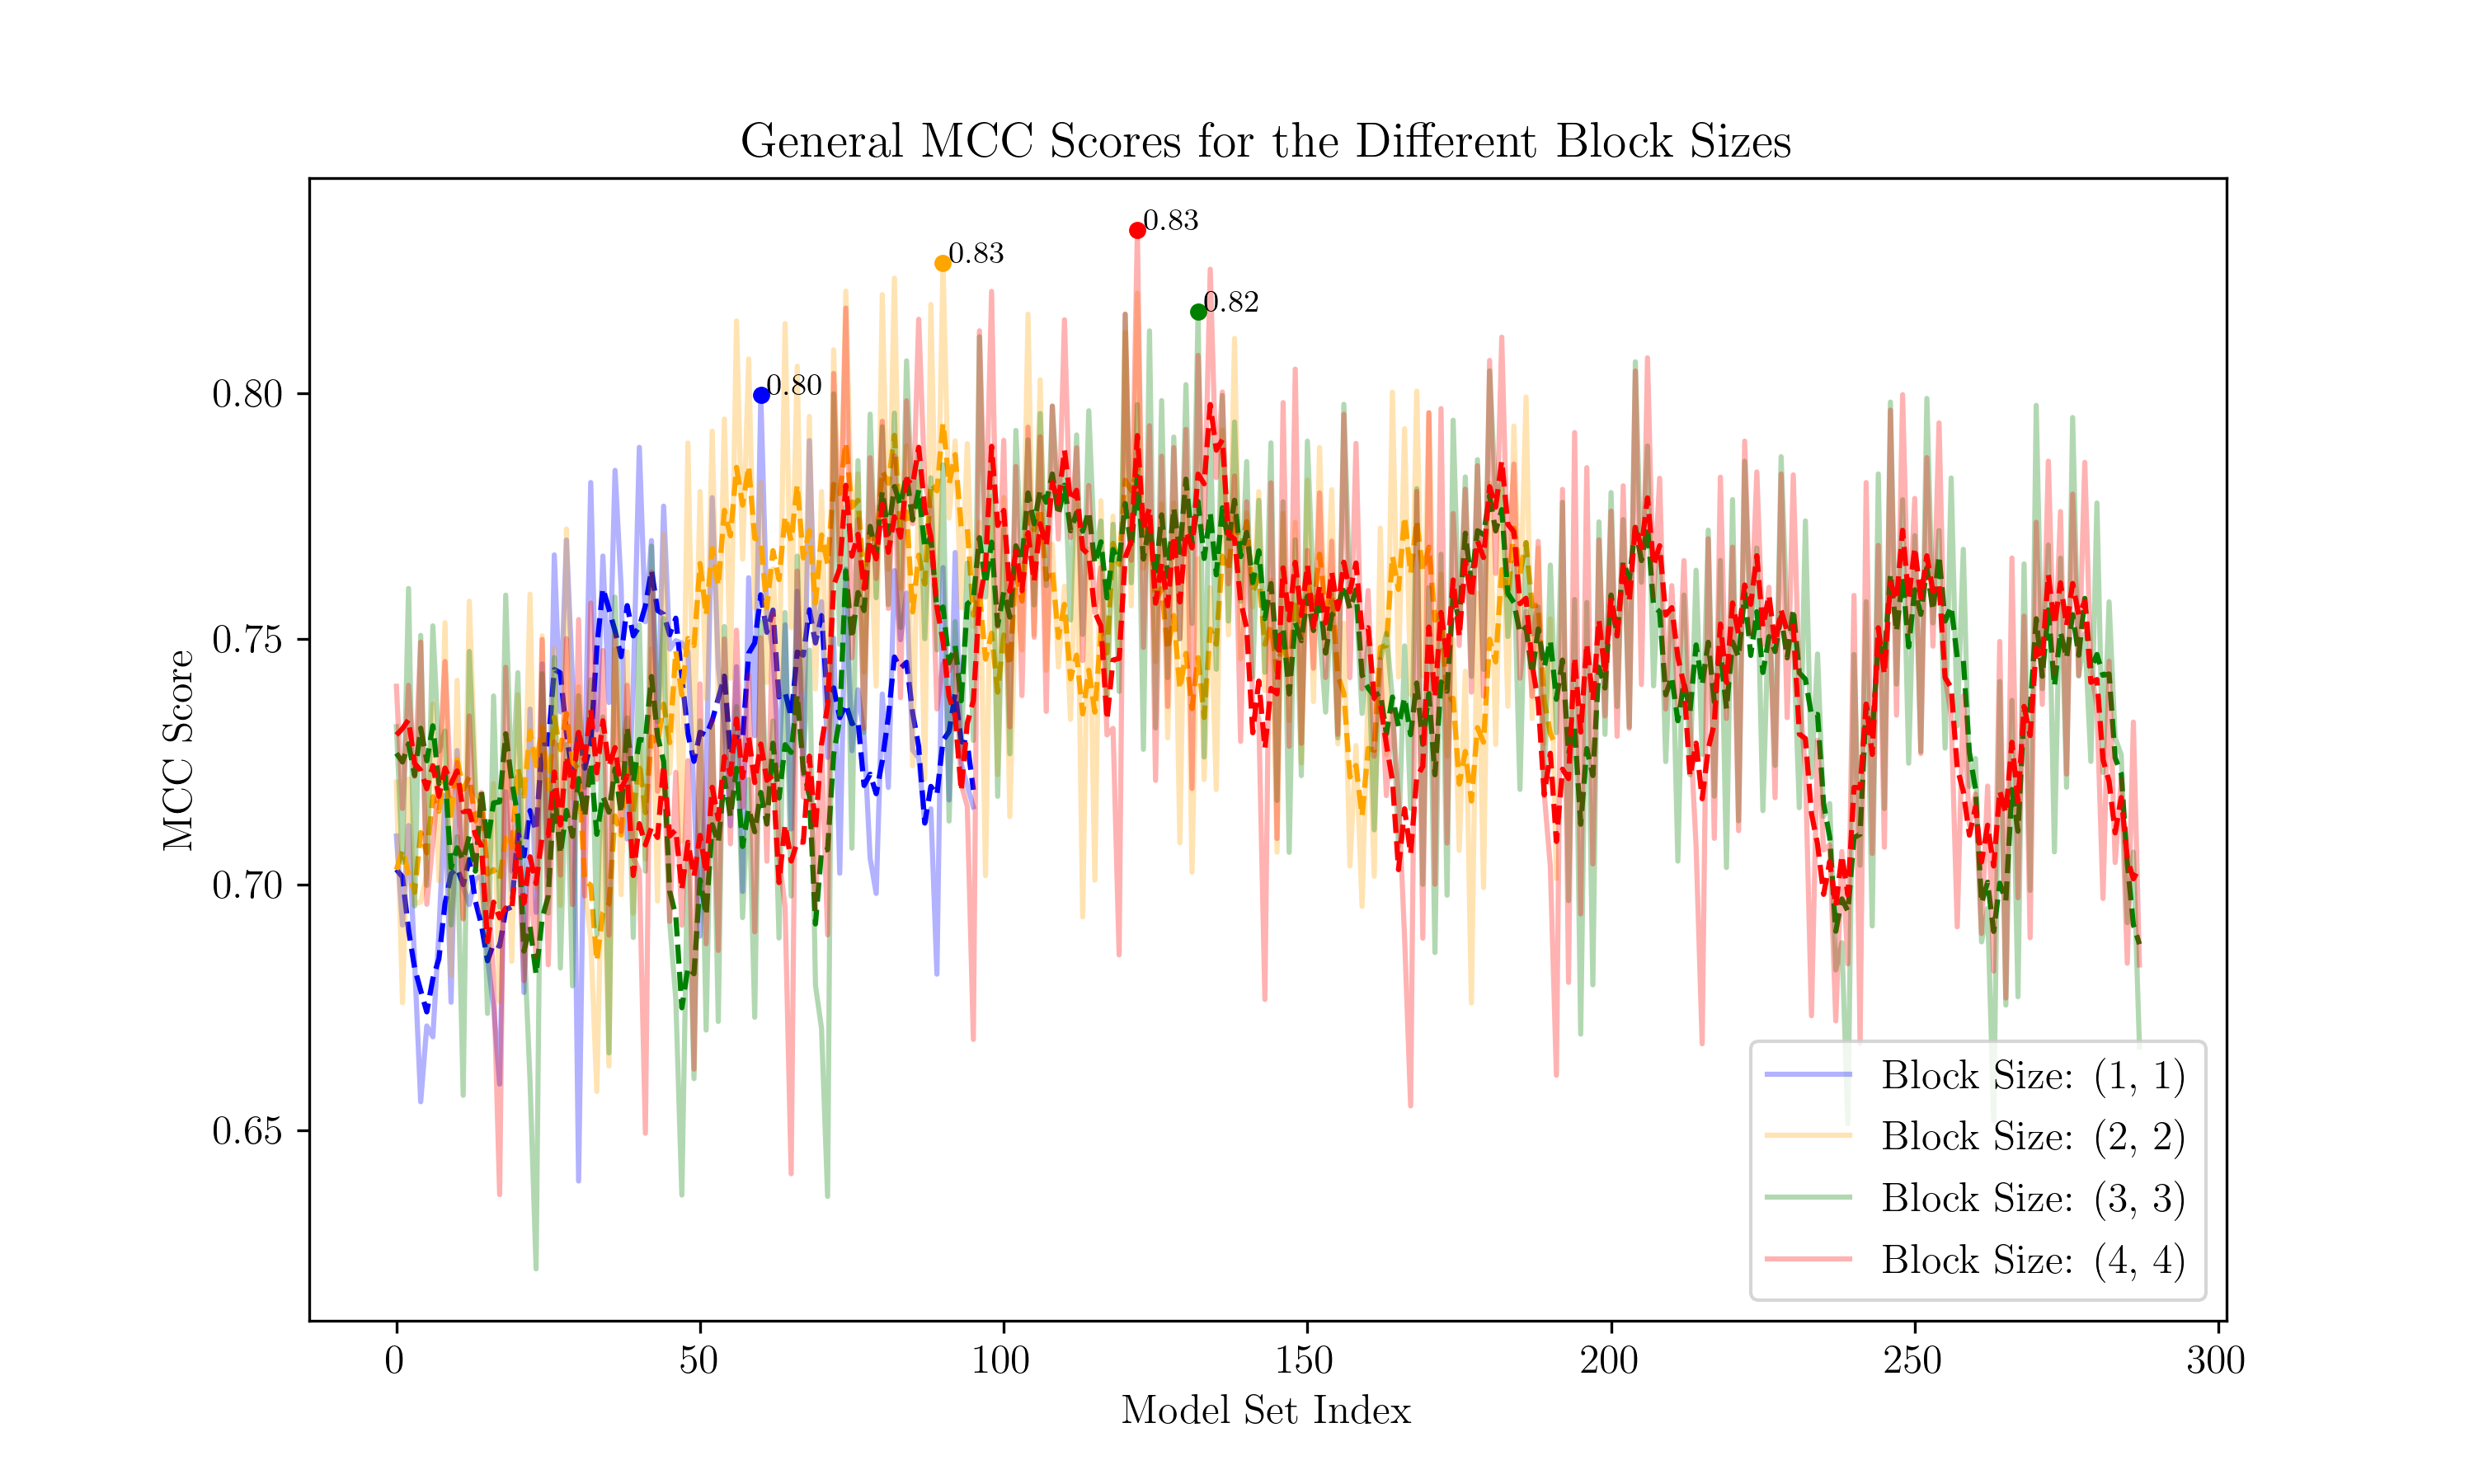
\includegraphics[width=0.9\linewidth]{mcc_block_size_total.png}
    \caption{
        MCC scores for the aggregate test dataset, grouped by block size.
    }
    \label{fig:block_size_total}
\end{figure}


\begin{figure}
    \centering
    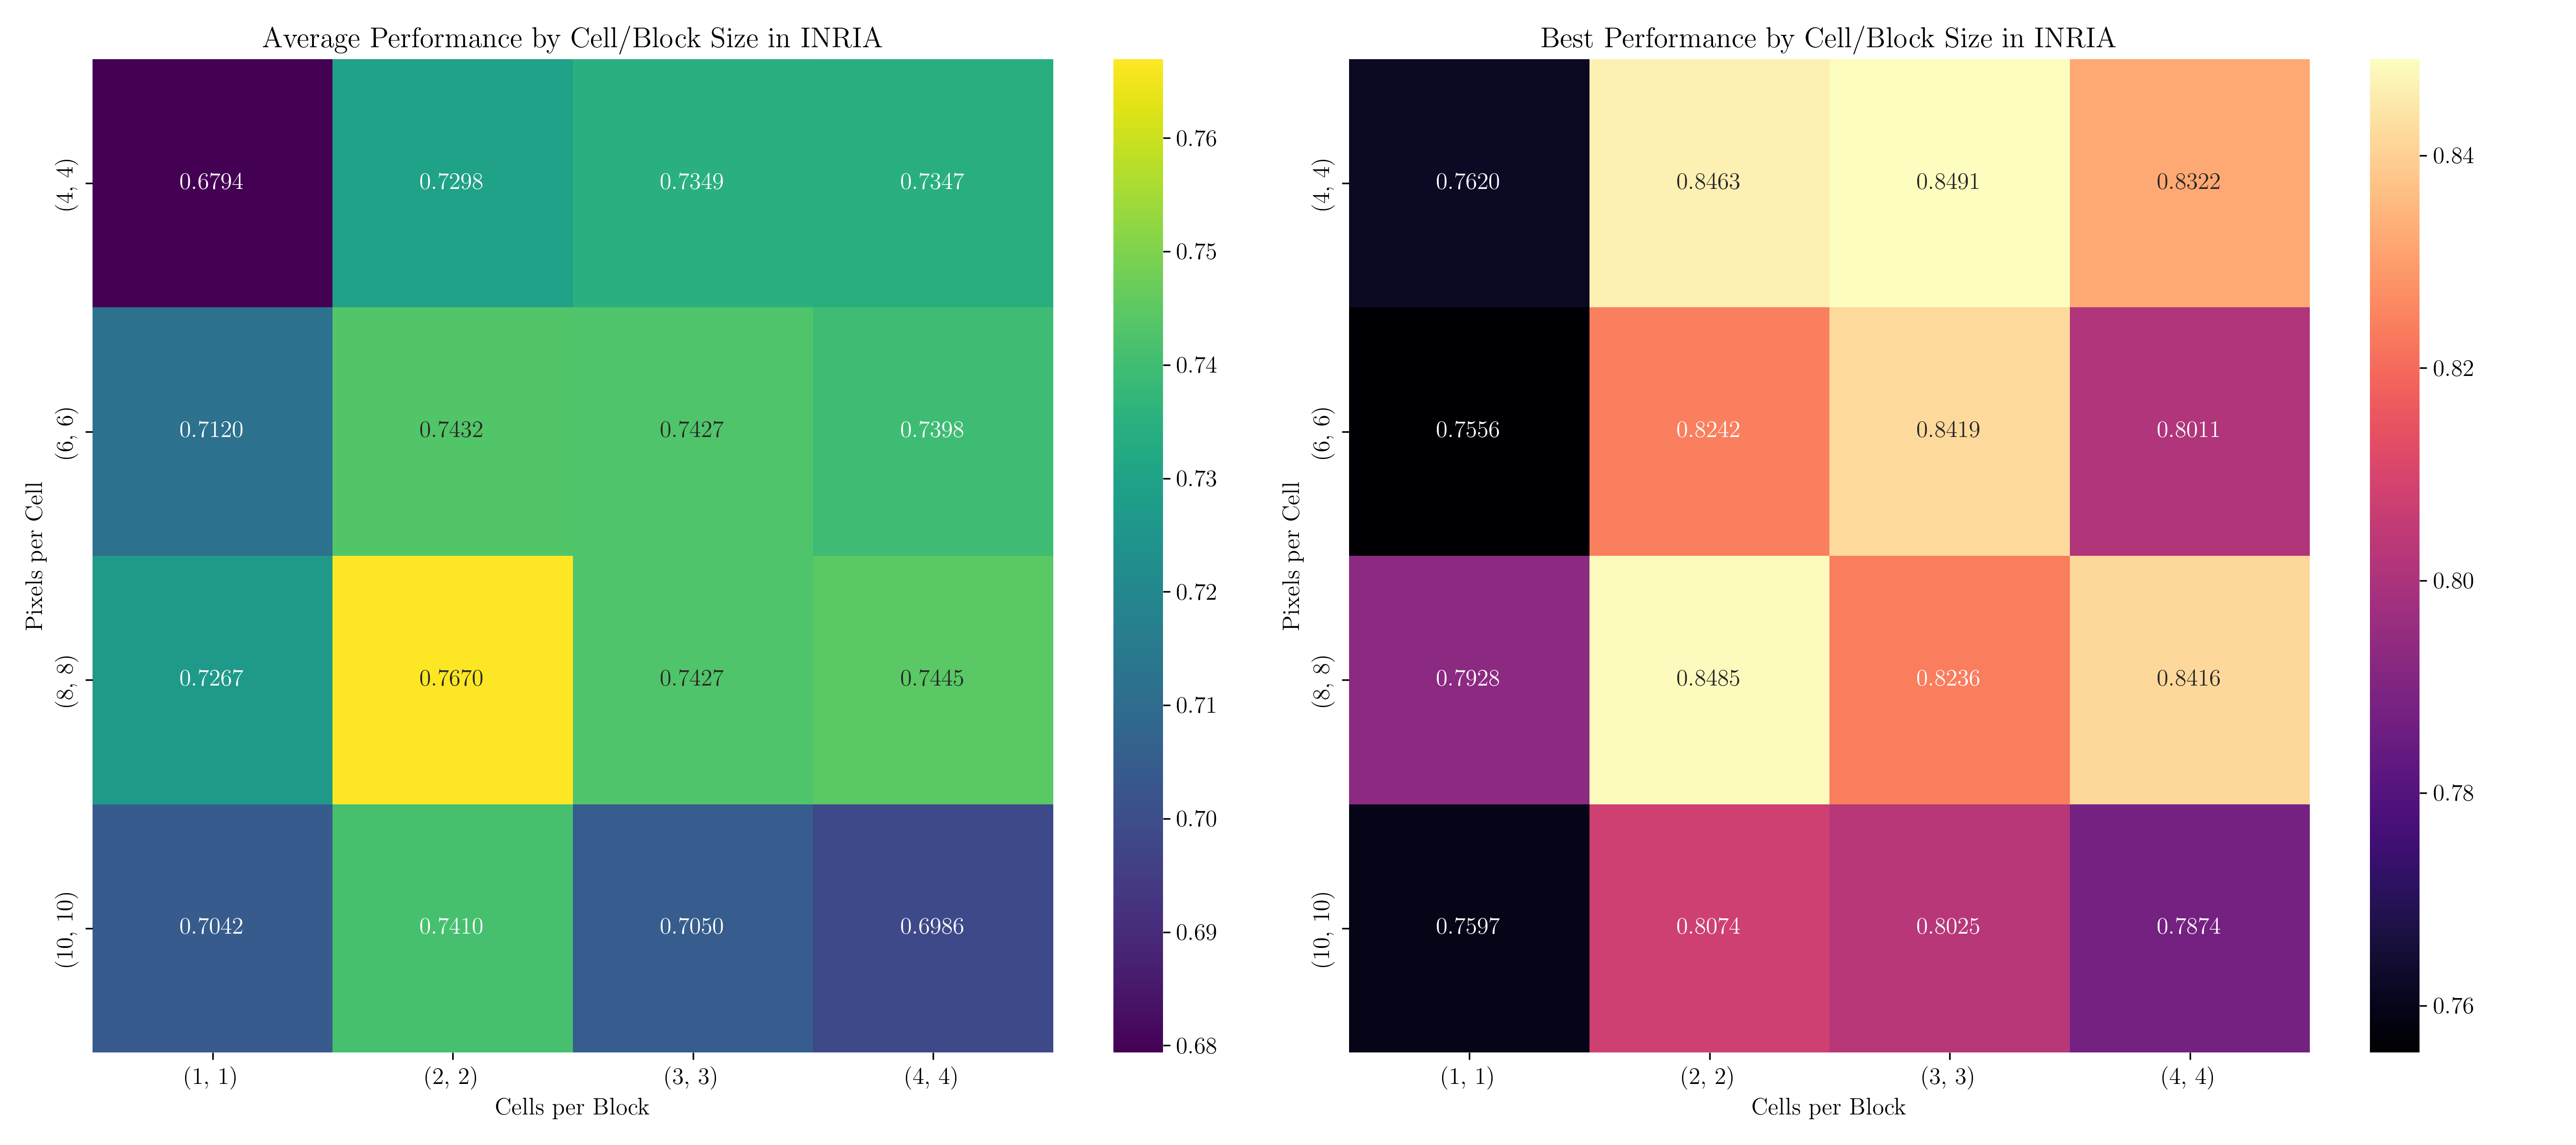
\includegraphics[width=\linewidth]{mcc_cell_block_heatmap_INRIA.png}
    \caption{
        A heatmap of MCC scores for the INRIA dataset, grouped by cell size and block size.
    }
    \label{fig:cell_block_heatmap_inria}
\end{figure}

\begin{figure}
    \centering
    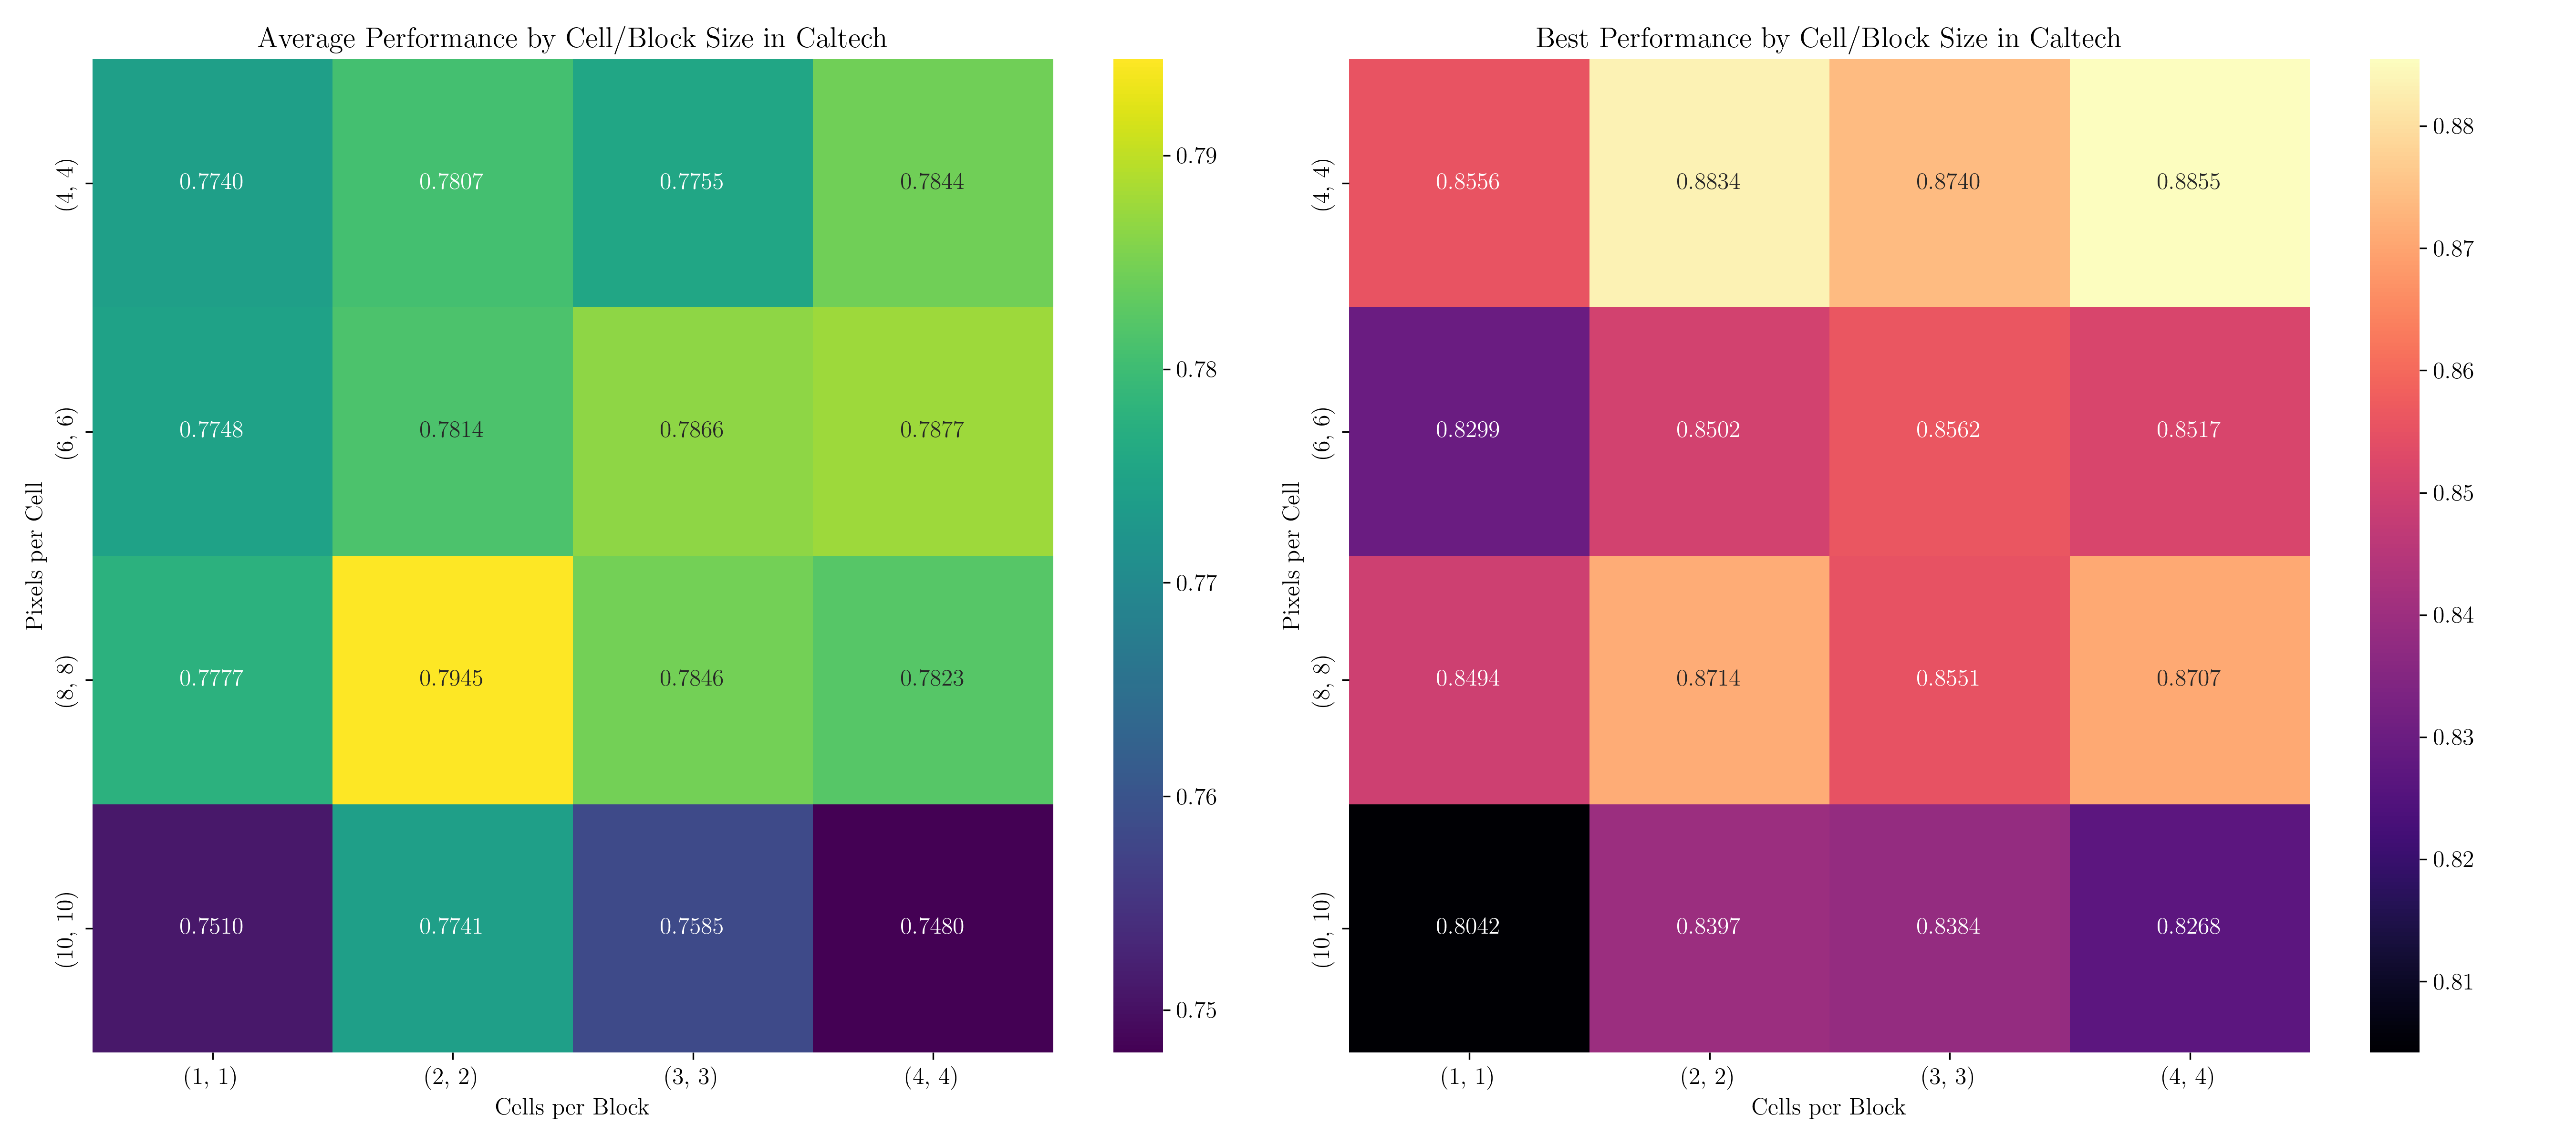
\includegraphics[width=\linewidth]{mcc_cell_block_heatmap_caltech_30.png}
    \caption{
        A heatmap of MCC scores for the Caltech dataset, grouped by cell size and block size.
    }
    \label{fig:cell_block_heatmap_caltech}
\end{figure}

\begin{figure}
    \centering
    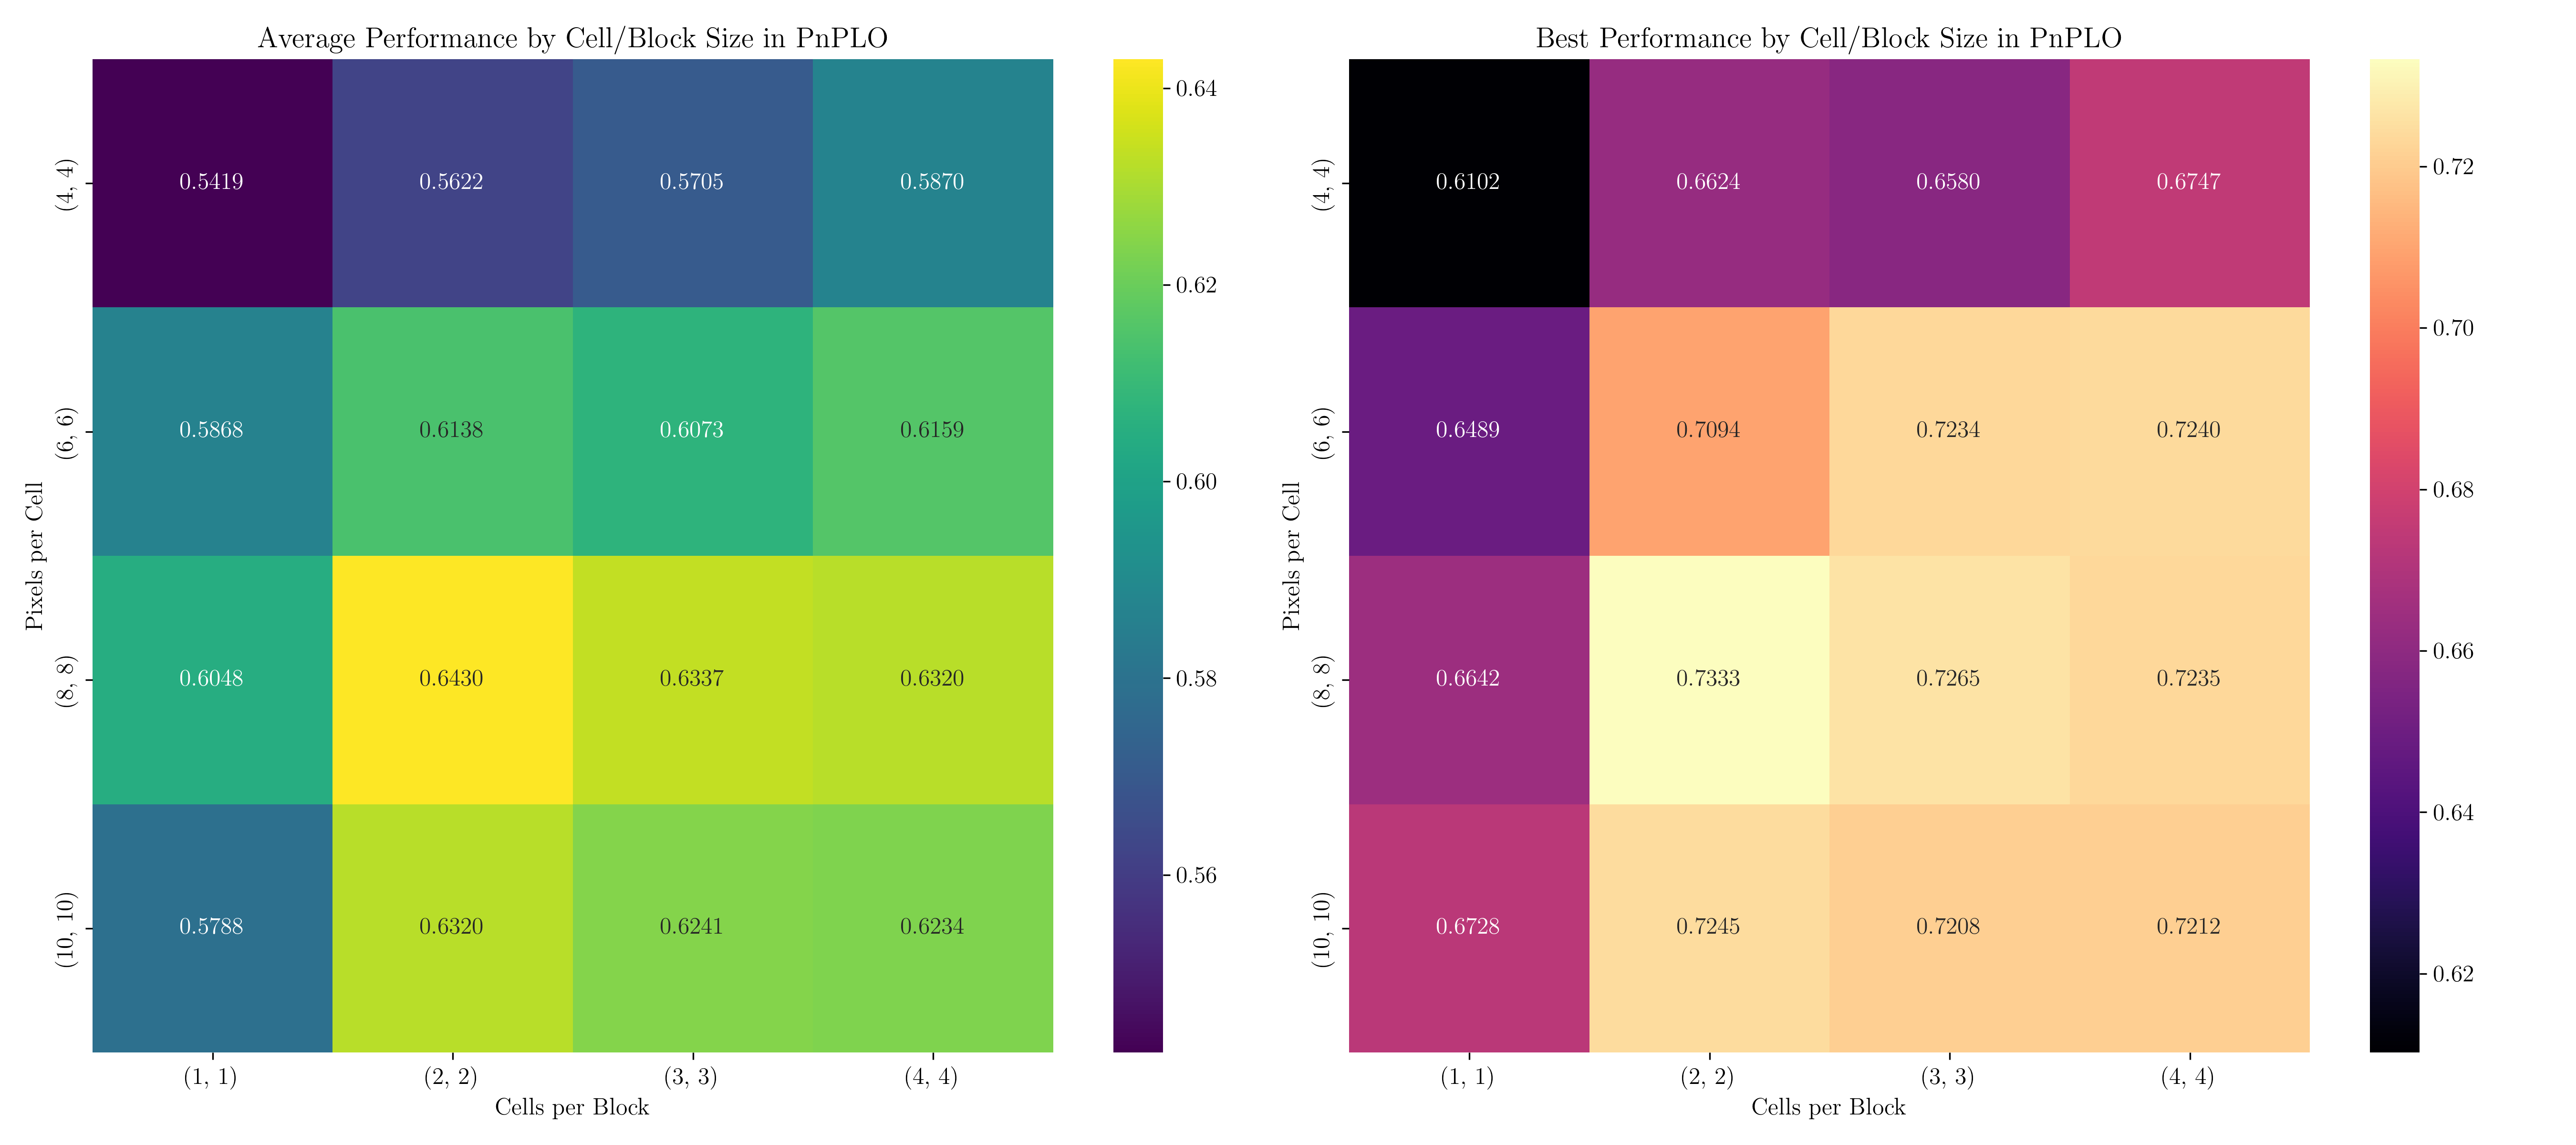
\includegraphics[width=\linewidth]{mcc_cell_block_heatmap_PnPLO.png}
    \caption{
        A heatmap of MCC scores for the PnPLO dataset, grouped by cell size and block size.
    }
\end{figure}

\begin{figure}
    \centering
    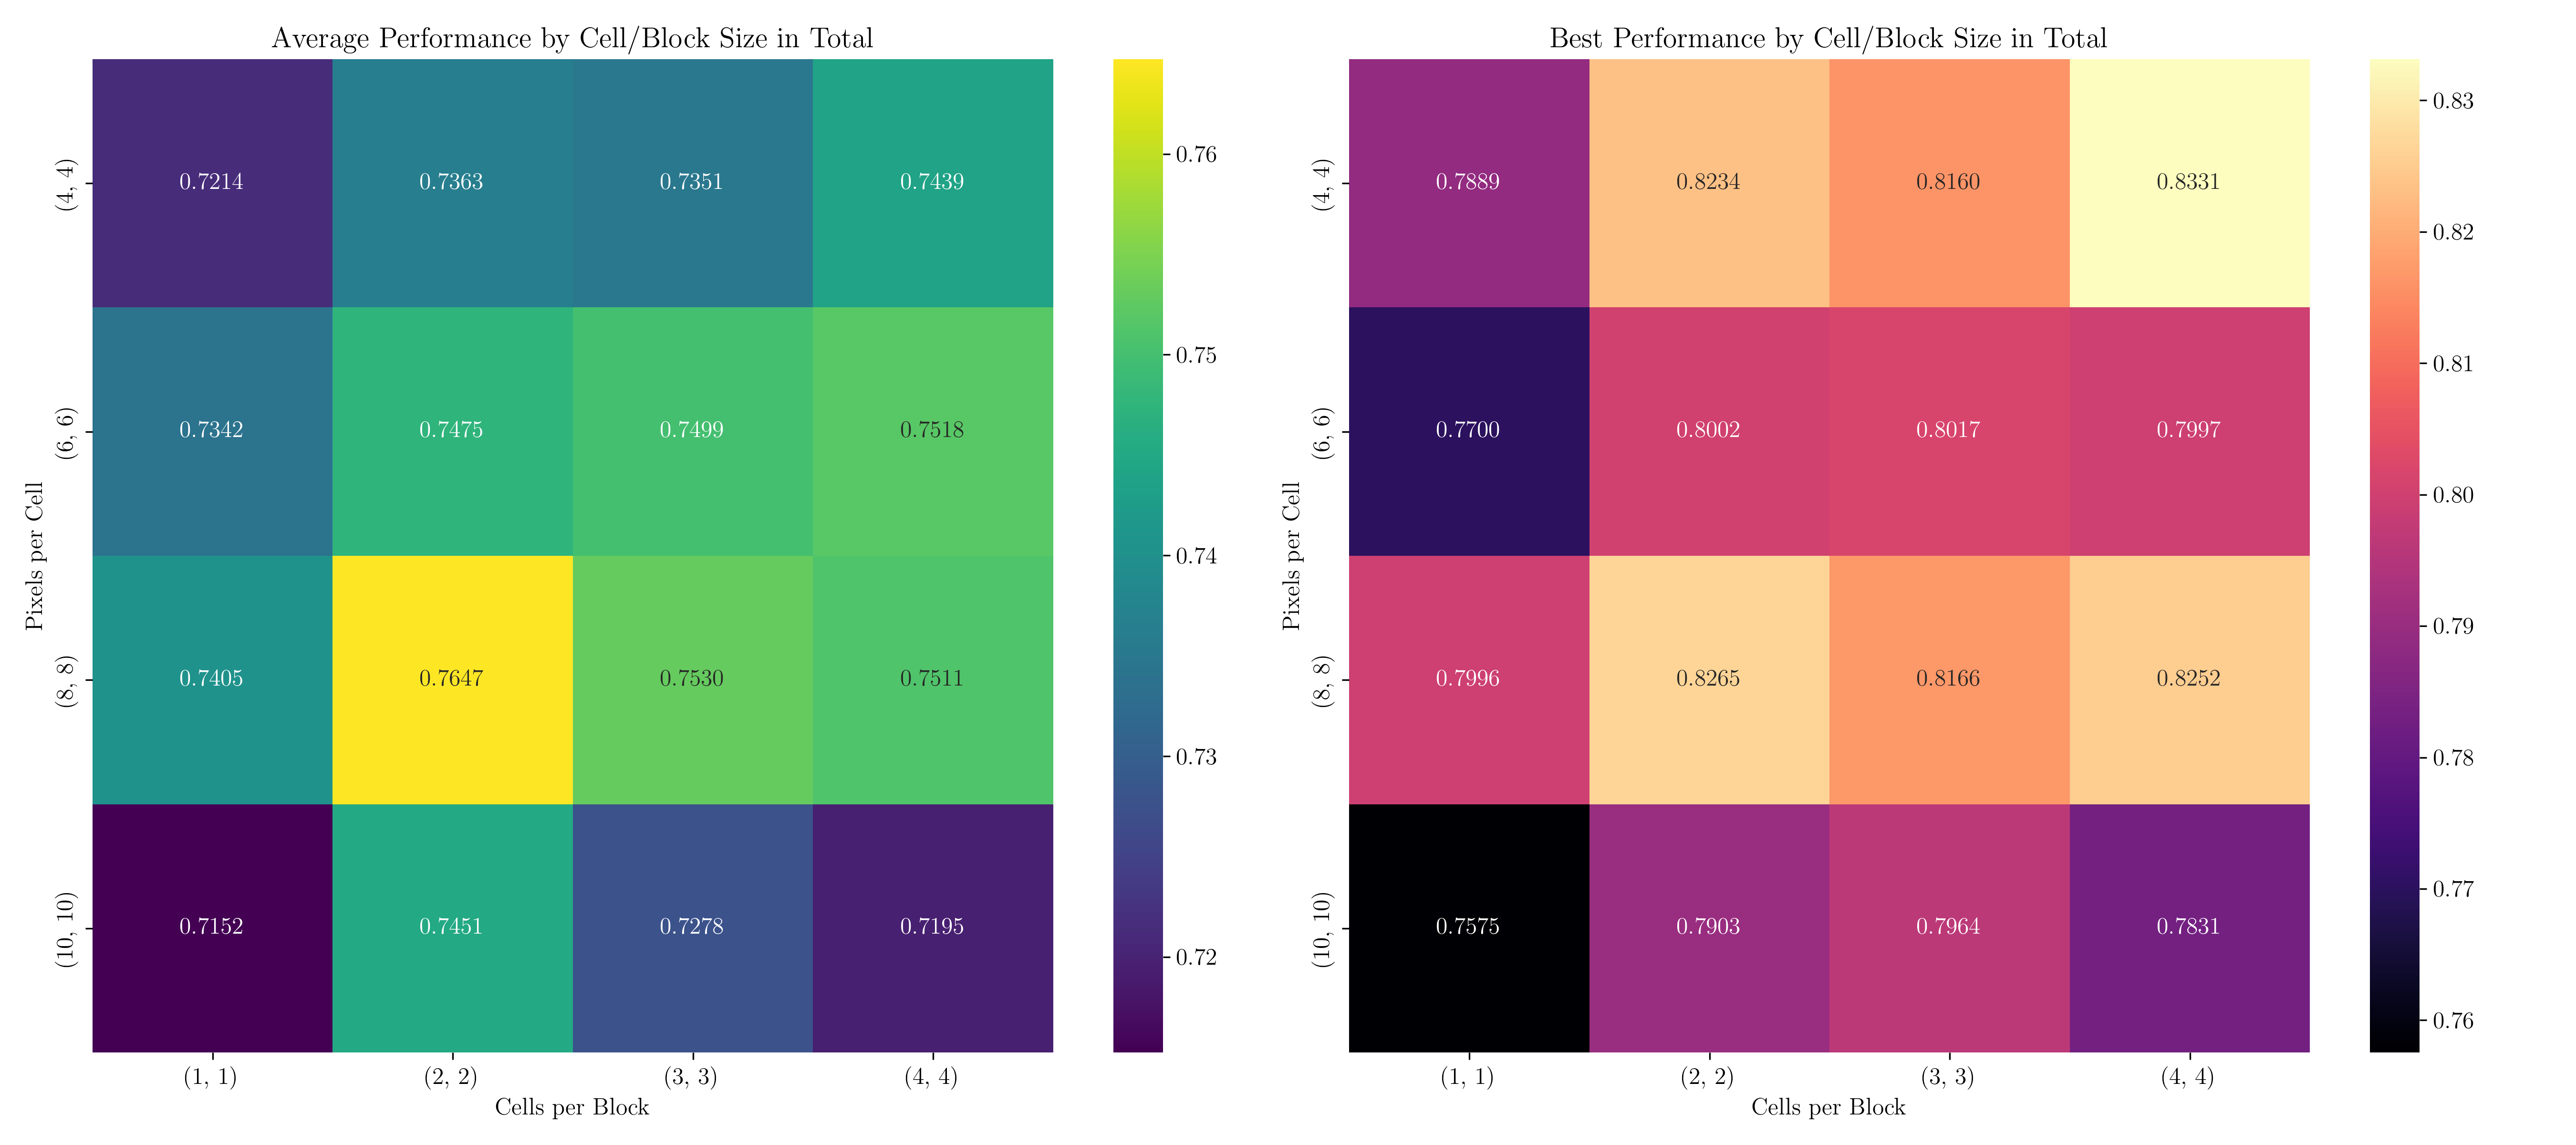
\includegraphics[width=\linewidth]{mcc_cell_block_heatmap_total.png}
    \caption{
        A heatmap of MCC scores for the aggregate test dataset, grouped by cell size and block size.
    }
    \label{fig:cell_block_heatmap_total}
\end{figure}

\subsubsection{Graphs for Block Sizes with Different Block Strides}

\begin{figure}
    \centering
    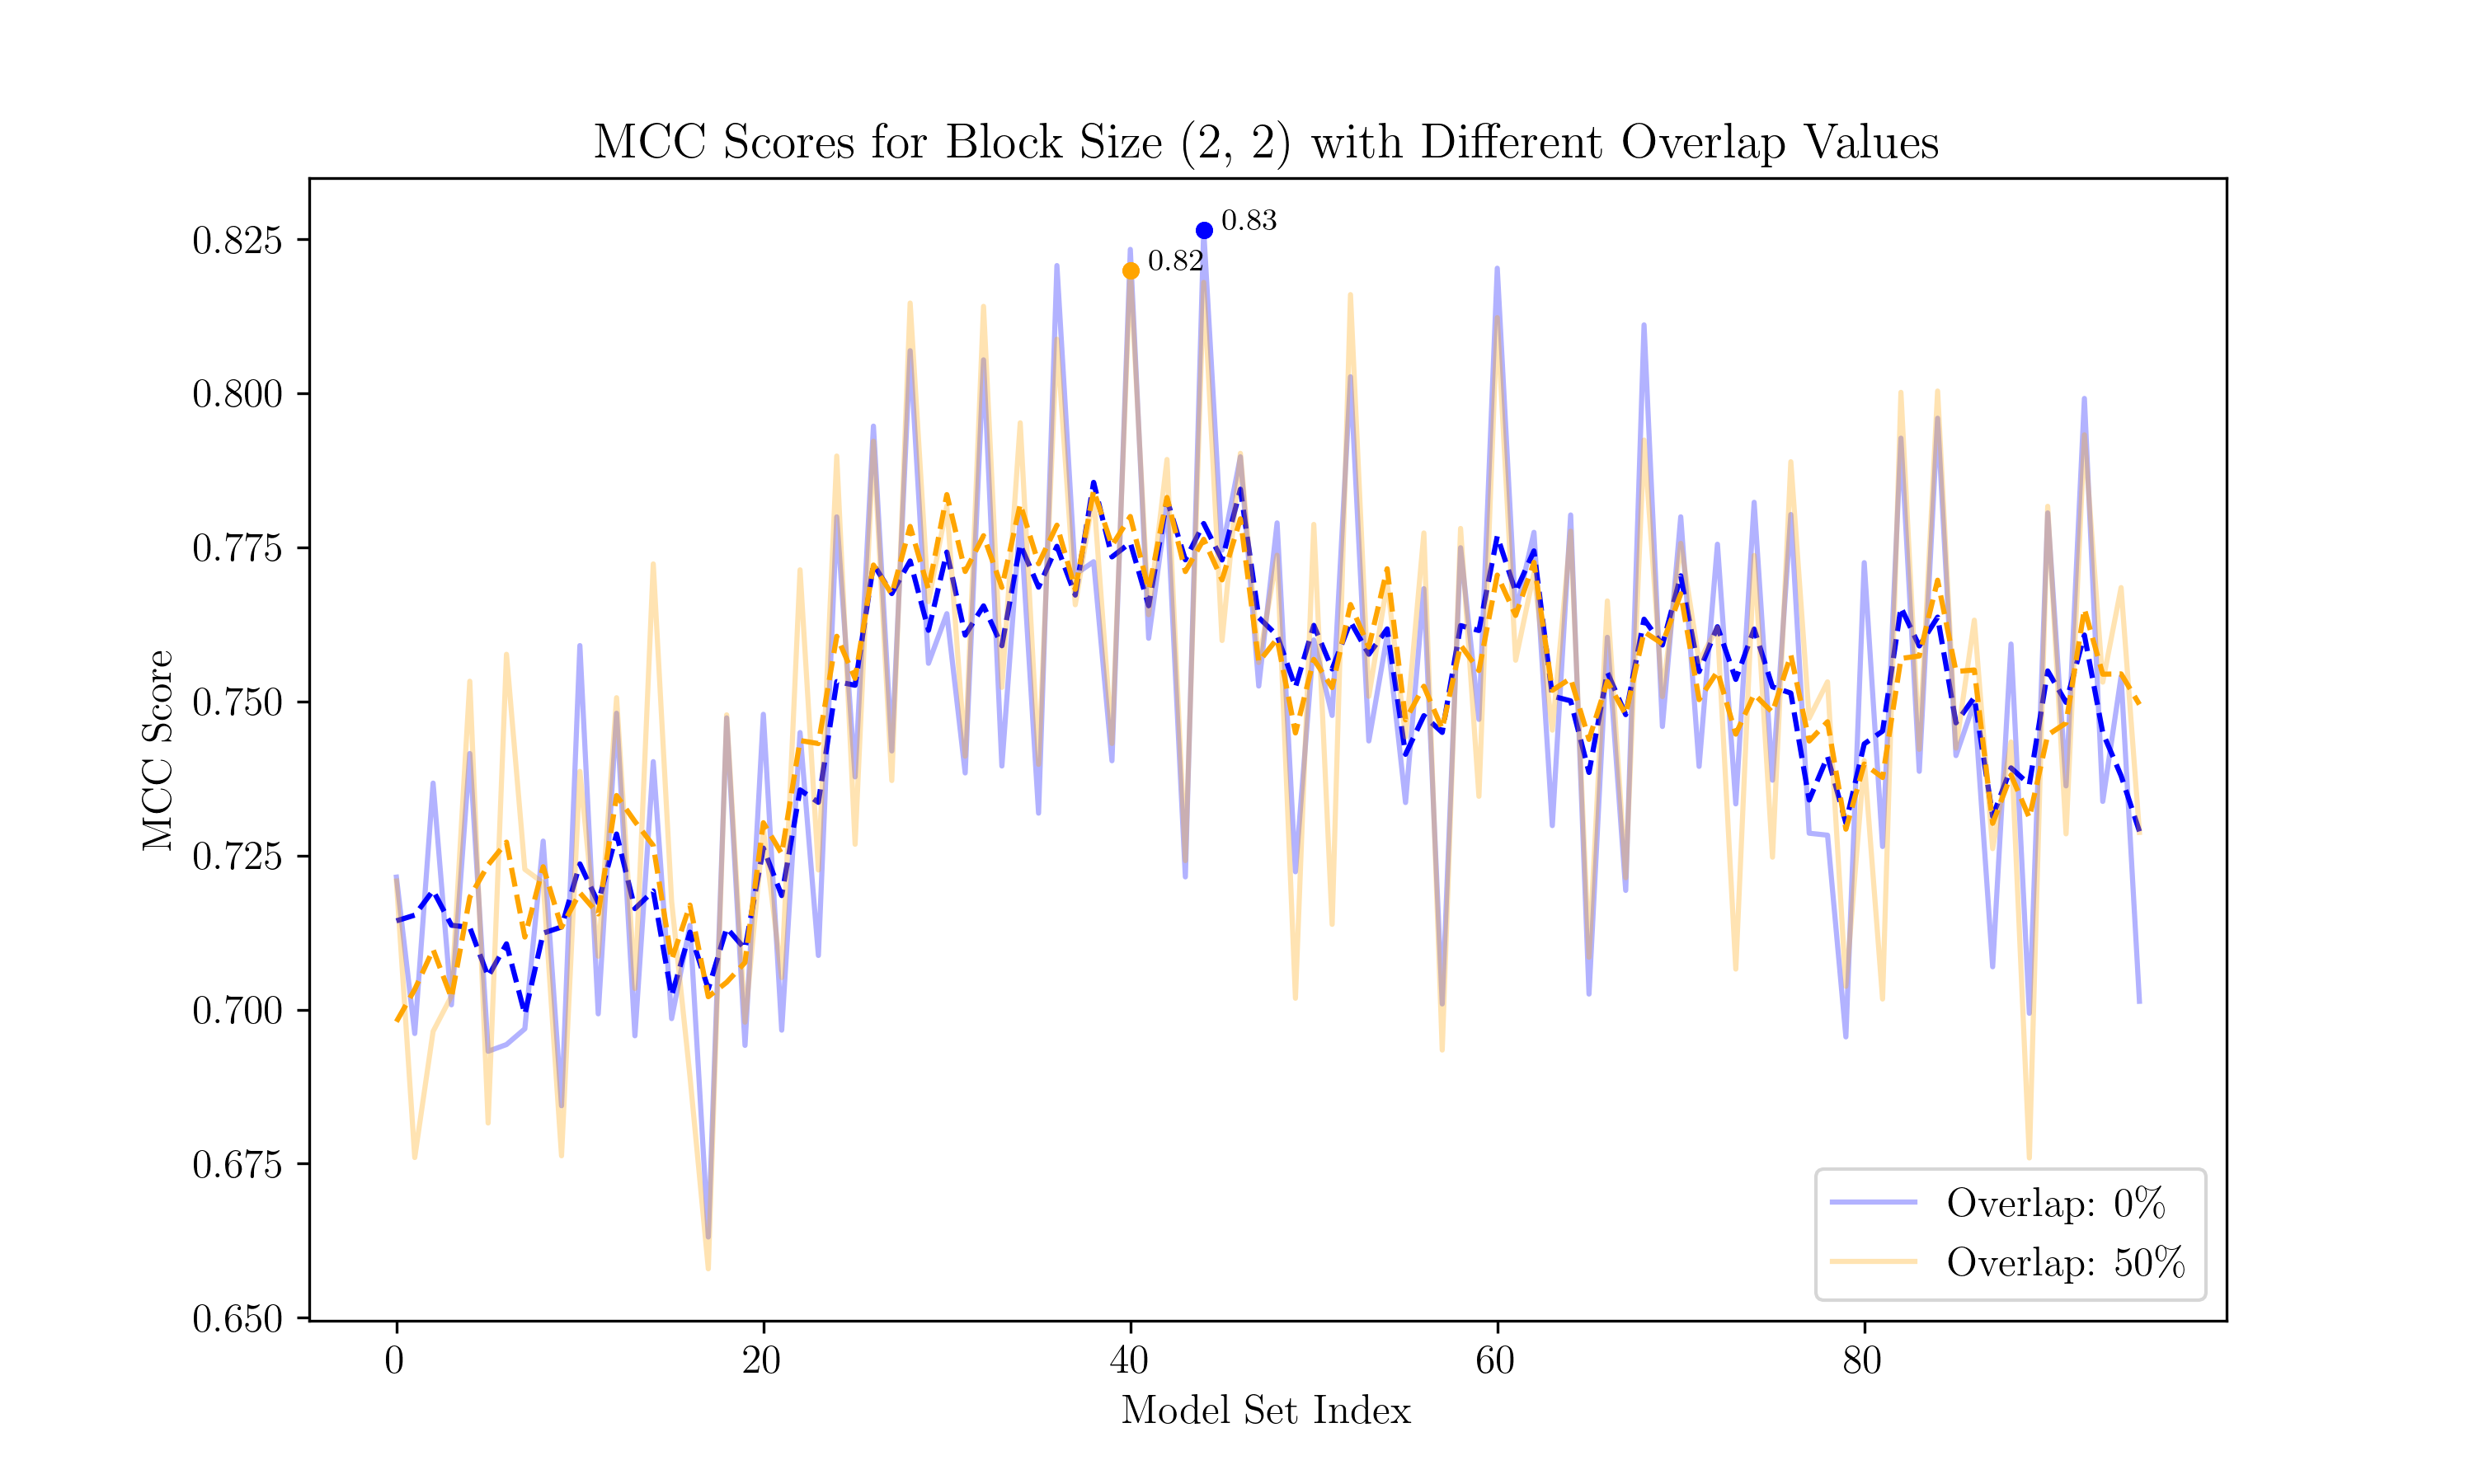
\includegraphics[width=0.9\linewidth]{mcc_overlap_(2, 2).png}
    \caption{
        MCC scores for the aggregate test dataset, grouped by block stride. The block size is set to (2, 2).
    }
    \label{fig:overlap_2_2}
\end{figure}

\begin{figure}
    \centering
    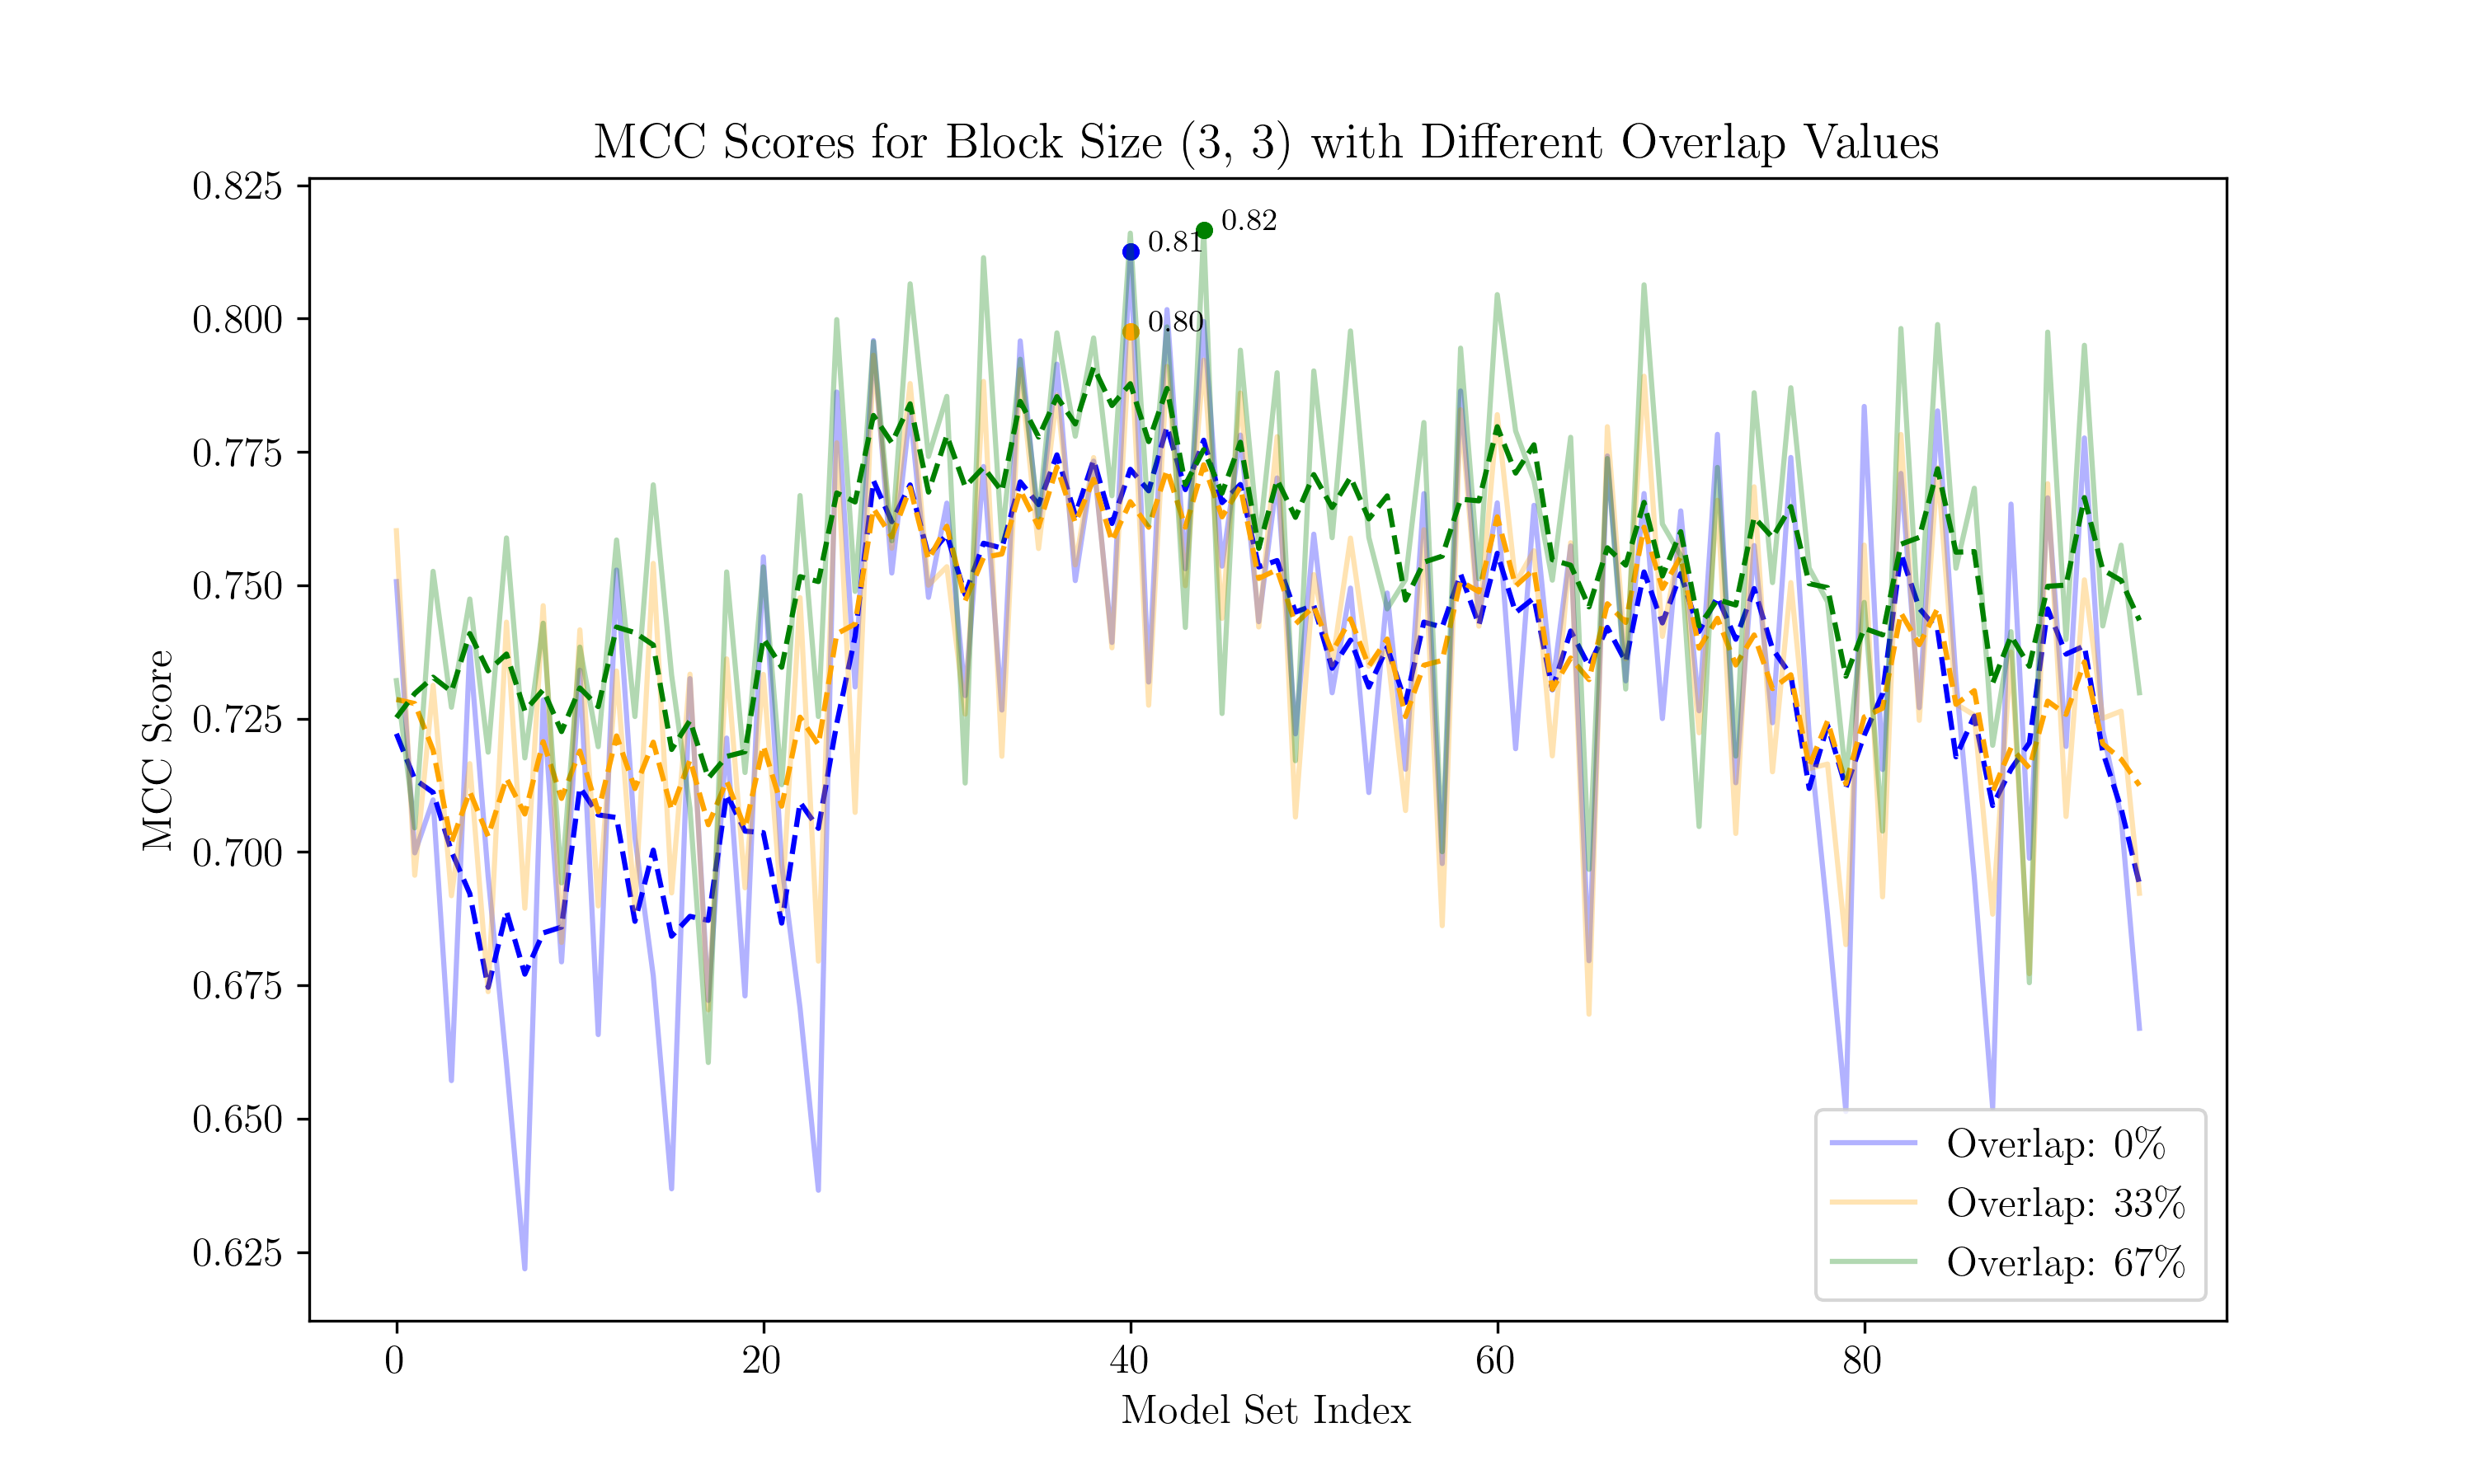
\includegraphics[width=0.9\linewidth]{mcc_overlap_(3, 3).png}
    \caption{
        MCC scores for the aggregate test dataset, grouped by block stride. The block size is set to (3, 3).
    }
    \label{fig:overlap_3_3}
\end{figure}

\begin{figure}
    \centering
    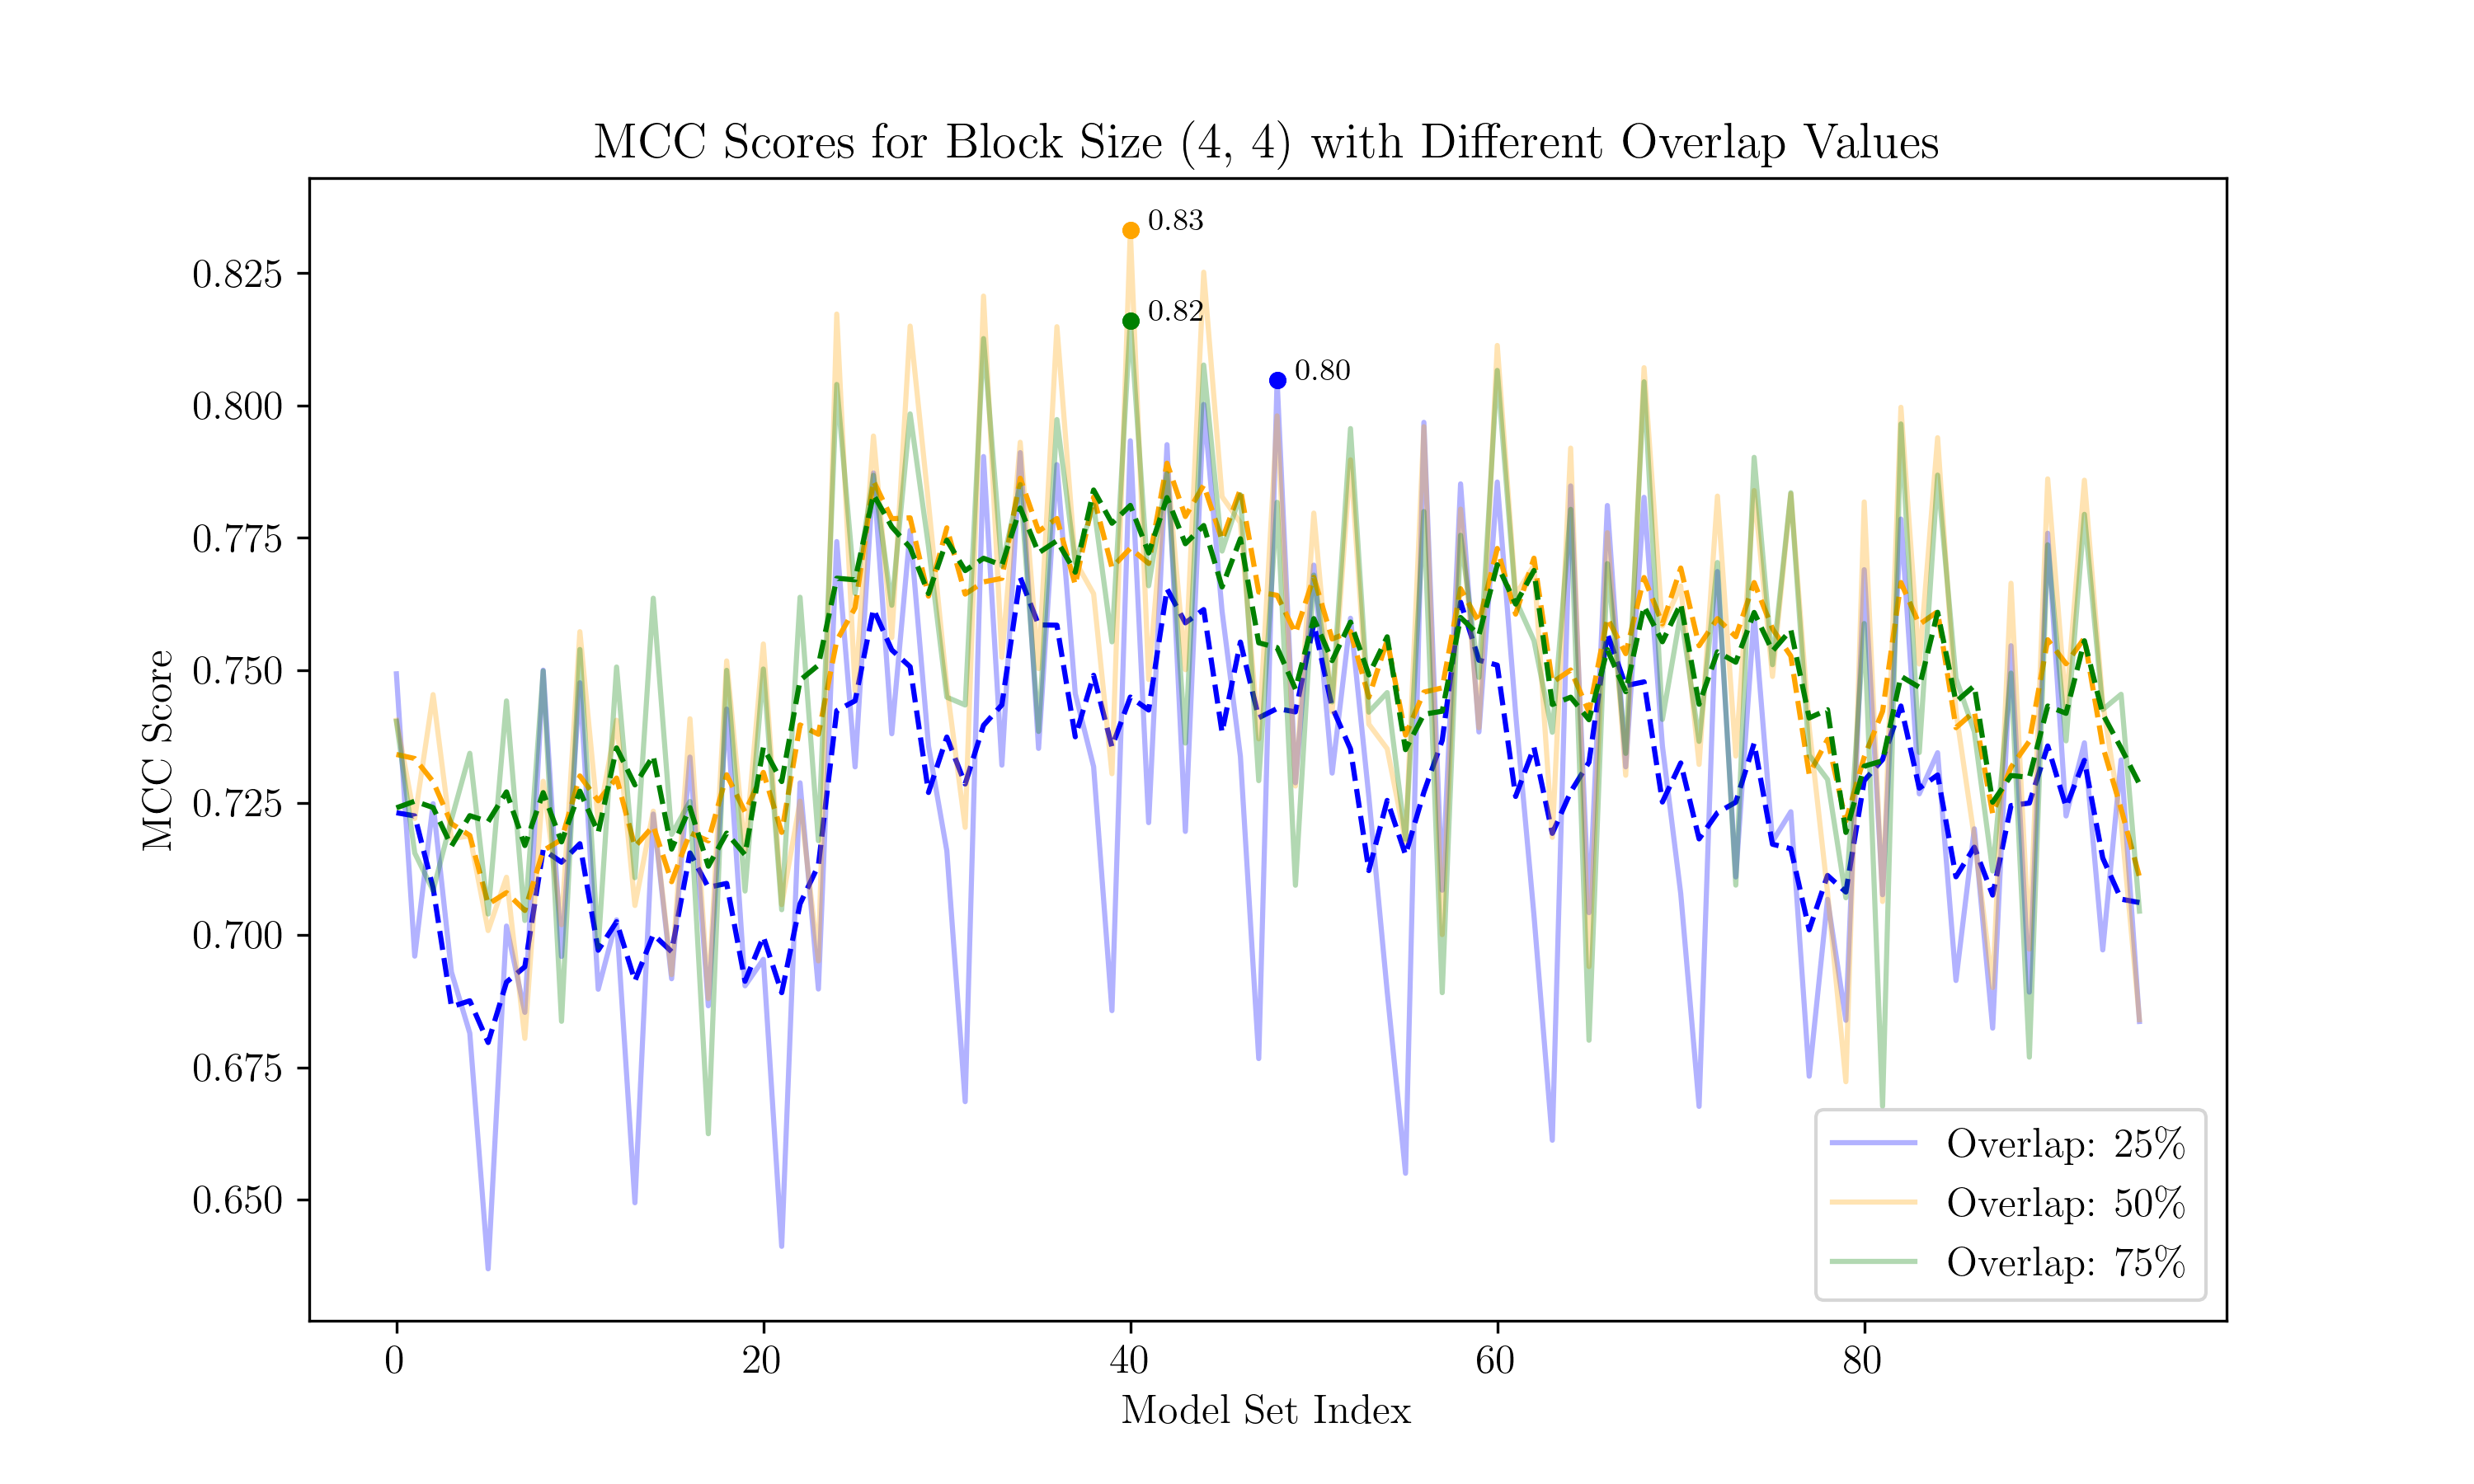
\includegraphics[width=0.9\linewidth]{mcc_overlap_(4, 4).png}
    \caption{
        MCC scores for the aggregate test dataset, grouped by block stride. The block size is set to (4, 4).
    }
    \label{fig:overlap_4_4}
\end{figure}

\subsection{Correlation Between Dimensionality and Time of Computation}

\begin{figure}
    \includesvg[width=\linewidth]{correlation_with_best_fit.svg}
    \caption{
        A scatter plot of the correlation between dimensionality and time of computation, with a best-fit line.
    }
    \label{fig:correlation_with_best_fit}
\end{figure}